\documentclass[a4paper,twoside,DIV15,BCOR12mm]{scrbook}

\usepackage{mathe}
\usepackage{saetze-baeuerle}
\usepackage{faktor}
\usepackage{enumerate}
\usepackage{tikz}
\usepackage{german}

\usepackage{remreset}
\makeatletter
\@removefromreset{section}{chapter}
\makeatother

\newcommand{\cF}{\mathcal F}
\newcommand{\borel}{{\mathfrak B}}

\author{Die Mitarbeiter von \url{http://mitschriebwiki.nomeata.de/}}
\title{Stochastische Prozesse}
\makeindex

\begin{document}
\maketitle
 
\newenvironment{enuma}{%
\begin{enumerate}[\hspace{1em}a)]%
}{%
\end{enumerate}%
}

\newenvironment{enumi}{%
\begin{enumerate}[\hspace{1em}i)]%
}{%
\end{enumerate}%
}

\setcounter{secnumdepth}{-1}
%\renewcommand{\thechapter}{\arabic{chapter}}
%\chapter{Inhaltsverzeichnis}
%\stepcounter{chapter}
%\renewcommand{\tocname}{bla}
%\addcontentsline{toc}{chapter}{\protect\numberline {\thechapter}Inhaltsverzeichnis}
\addcontentsline{toc}{chapter}{Inhaltsverzeichnis}
\tableofcontents

 % Vorwort

\chapter{Vorwort}
\setcounter{secnumdepth}{2}
%\addcontentsline{toc}{chapter}{Vorwort}

\section*{Über dieses Skriptum}
Dies ist ein Mitschrieb der Vorlesung \glqq Stochastische Prozesse\grqq\ von Prof. Dr. Bäuerle im
Sommersemester 08 an der Universität Karlsruhe (TH).
Die Mitschriebe der Vorlesung werden mit ausdrücklicher Genehmigung von Prof Dr. Bäuerle hier veröffentlicht,
Prof. Dr. Bäuerle ist für  den Inhalt nicht verantwortlich.
\section*{Wer}
Gestartet wurde das Projekt von Joachim Breitner.
Weiter haben Felix Wellen und Michael Walter beim Mitschreiben geholfen.

\section*{Wo}
Alle Kapitel inklusive \LaTeX-Quellen können unter \url{http://mitschriebwiki.nomeata.de} abgerufen werden.
Dort ist ein von Joachim Breitner programmiertes \emph{Wiki}, basierend auf \url{http://latexki.nomeata.de} installiert. 
Das heißt, jeder kann Fehler nachbessern und sich an der Entwicklung
beteiligen. Auf Wunsch ist auch ein Zugang über \emph{Subversion} möglich.

%\setcounter{chapter}{0}
%\renewcommand{\thesection}{{\rm\bfseries §}\arabic{section}}
\renewcommand{\thesection}{\arabic{section}}
\renewcommand{\thechapter}{\Roman{chapter}}

\chapter{Markov-Ketten mit diskretem Zeitparameter}

\section{Elementare Eigenschaften von Markov-Ketten}

Gegeben sei eine Folge von Zufallsvariablen $(X_n)$ auf dem Wahrscheinlichkeitsraum $(\Omega, \cF, P)$ mit $X_n:\Omega \to S$ wobei $S$ nicht leer, und endlich oder abzählbar unendlich ist.

\begin{definition}
Eine $S\times S$-Matrix $P=(p_{ij})$ heißt \emph{stochastische Matrix}\index{stochastische Matrix}, falls $p_{ij}\ge0$ ist und für alle $i\in S$ die Zeilensumme $\sum_{j\in S} p_{ij} = 1$ ist.
\end{definition}

\begin{definition}
Sei $P$ eine stochastische Matrix. Eine (endliche oder unendliche) Folge $X_0, X_1, X_2,\ldots$ von $S$-wertigen Zufallsvariablen heißt (homogene\footnote{kurz für zeit-homogen. Die Übergangswahrscheinlichkeiten hängen nicht vom aktuellen Zeitpunkt ab.}) \emph{Markov-Kette}\index{Markov-Kette!zeitdiskrete} mit Übergangsmatrix $P$, falls für alle $n\in \MdN$\footnote{Hier ist $\MdN=1,2,\ldots$} und für alle Zustände $i_k\in S$ mit 
\[
P(X_0=i_0,\ldots,X_n=i_n) >0
\]
gilt
\[
P(X_{n+1} = i_{n+1} \mid X_0 = i_0, \ldots, X_n=i_n) = 
P(X_{n+1} = i_{n+1} \mid X_n=i_n)\da p_{i_n i_{n+1}}.
\]

Die $p_{ij}$ heißen Übergangswahrscheinlichkeiten und die \emph{Startverteilung} $\nu$ der Kette ist definiert durch $\nu(i)\da P(X_0=i)$ für $i\in S$.
\end{definition}

\begin{bemerkung}
Jede Folge von unabhängigen Zufallsvariablen ist eine Markov-Kette.
\end{bemerkung}

\begin{satz}[Eigenschaften von Markov-Ketten]
$(X_n)$ ist genau dann eine Markov-Kette mit Übergangsmatrix $P$, falls gilt:
\[
P(X_k = i_k,\, 0\le k\le n) = P(X_0 = i_0)\prod_{k=0}^{n-1} p_{i_k i_{k+1}} \quad \forall n\in \MdN_0 \ \forall i_k\in S
\]
genau dann wenn gilt:
\[
P(X_k = i_k,\, 1\le k\le n \mid X_0=i_0) = \prod_{k=0}^{n-1} p_{i_k i_{k+1}} \quad \forall n\in \MdN_0 \ \forall i_k\in S\text{ mit $P(X_0=i_0)>0$}
\]
genau dann wenn gilt:
\[
P(X_k = i_k,\,m\le k\le m+n) = P(X_m=i_m)\prod_{k=m}^{m+n-1} p_{i_k i_{k+1}} \quad \forall m,n\in \MdN_0 \ \forall i_k\in S
\]
\end{satz}

\begin{beweis}
Zur ersten Äquivalenz. Sei $A_k \da [X_k=i_k]$, $k\in\MdN_0$.

„$\Longrightarrow$“ Induktion über $n$: $n=0$ $\checkmark$, $n\curvearrowright n+1:$ 
\begin{align*}
P(A_0A_1\ldots A_nA_{n+1}) &= P(A_0\ldots A_n)\cdot P(A_{n+1}\mid A_0\ldots A_n) \\
&= P(A_0\ldots A_n)\cdot p_{i_ni_{n+1}} && \text{(Markov-Eigenschaft)}\\
&= P(X_0=i_0)\prod_{k=0}^n p_{i_ki_{k+1}} && \text{(I.V.)}
\end{align*}

„$\Longleftarrow$“ 
\begin{align*}
P(A_{n+1}\mid A_0\ldots A_n) &= \frac{P(A_0\ldots A_nA_{n+1})}{P(A_0\ldots A_n)} \\
&= p_{i_ni_{n+1}} && \text{(Vor.)}
\end{align*}
Die weiteren Äquivalenzen sind ähnlich zu beweisen.
\end{beweis}

\paragraph{Konstruktion einer Markov-Kette.} Seien $(Y_n)$ Zufallsvariablen, unabhängig und identisch verteilt (u.i.v.), in $Z$. Weiter ist $g:S\times Z\to S$ eine messbare Abbildung. Definiere die Folge $(X_n)$ mit 
\[X_0=c\in S, \quad X_n = g(X_{n-1},Y_n).\]
Die so konstruierte Folge $(X_n)$ ist eine Markov-Kette mit Werten in $S$ und Übergangsmatrix $P=(p_{ij})$ mit $p_{ij} = P(g(i,Y_n)=j)$.

\begin{beweis}
Die Variablen $X_0,\ldots,X_n$ hängen nur von $X_0,Y_1,\ldots,Y_n$ ab, sind also unabhängig von $Y_{n+1}$.
\begin{align*}
P(X_{n+1} = i_{n+1} \mid X_k = i_k, 0\le k\le n) 
&= \frac{P(X_k = i_k,\, 0\le k\le n+1)}{P(X_k = i_k,\, 0\le k\le n)} \\
&= \frac{P(X_k = i_k,\, 0\le k\le n,\, g(i_n,Y_{n+1})=i_{n+1})}{P(X_k = i_k,\, 0\le k\le n)} \\
&= \frac{P(X_k = i_k,\, 0\le k\le n)\cdot P(g(i_n,Y_{n+1})=i_{n+1})}{P(X_k = i_k,\, 0\le k\le n)} \\
&= P(g(i_n,Y_{n+1})=i_{n+1}) \\
&= \frac{P(g(i_n,Y_{n+1})=i_{n+1})\cdot P(X_n=i_n)}{P(X_n =i_n)} \\
&= \frac{P(g(i_n,Y_{n+1})=i_{n+1}, X_n=i_n)}{P(X_n =i_n)} \\
&= P(g(i_n,Y_{n+1})=i_{n+1}\mid X_n=i_n) \\
&= P(X_{n+1} = i_{n+1} \mid X_n=i_n)
\end{align*}
\end{beweis}

\begin{bemerkung}
Umgekehrt kann zu jeder stochastischen Matrix $P$ eine Markov-Kette $(X_n)$ konstruiert werden mit $X_n=g(X_{n-1},Y_n)$, wobei $(Y_n)$ u.i.v. und o.B.d.A. $Y_n \sim U[0,1]$.
\end{bemerkung}

\begin{beispiel}[Lagerhaltung]
Sei $Y_n$ die Nachfrage nach einem gelagerten Produkt im Zeitintervall $(n-1,n]$. $(Y_n)$ sei u.i.v. und $Y_n\in \MdN_0$. Die Auffüll-Politik sei eine $(z,Z)$-Politik mit $z\le Z$, $z,Z\in \MdN$, die wie folgt funktioniert: Falls der Lagerbestand zur Zeit $n\le z$ ist, dann fülle auf $Z$ auf, sonst tue nichts.

Sei $X_n$ der Lagerbestand zum Zeitpunkt $n$, $S=\MdN_0$. Es gilt
\[
X_n =
\begin{cases}
(Z - Y_n)^+, & X_{n-1} \le z \\
(X_{n-1} - Y_n)^+, & X_{n-1} > z
\end{cases}
\]
Also ist $(X_n)$ eine Markov-Kette mit Übergangsmatrix $P=(p_{ij})$ und
\[
p_{ij} = 
\begin{cases}
P( (Z-Y_n)^+ = j), & i\le z \\
P( (i-Y_n)^+ = j), & i > z
\end{cases}
\]
\end{beispiel}

\begin{beispiel}[Ruinspiel]
Zwei Spieler mit Startkapital $B\in\MdN$ Euro spielen in Runden um jeweils einen Euro, etwa mit einem Münzwurf. Spieler I gewinnt dabei mit Wahrscheinlichkeit $p$. Sei $Y_n = 1$, falls Spieler I die $n$-te Runde gewinnt, und $Y_n= -1$, falls er die $n$-Runde verliert. Wir nehmen an, dass $Y_n$ u.i.v. ist.

Wir interessieren uns für das Kapital $X_n$ von Spieler I nach der $n$-ten Runde. Damit ist der Zustandsraum $S=\{0,1,\ldots,2B\}$.

Es gilt $X_0 = B$ und
\[
X_n = 
\begin{cases}
2B, &X_{n-1} = 2B \\
X_{n-1} + Y_n, & 0 < X_{n-1} < 2B \\
0, &X_{n-1} = 0.
\end{cases}
\]
Es folgt aus der Konstruktion direkt dass $(X_n)$ eine Markov-Kette ist mit Übergangsmatrix $P=(p_{ij})$, und
$p_{00} = p_{2B,2B} = 1$ sowie
\[
p_{ij} = 
\begin{cases}
p, &j=i+1\\
1-p, &j=i-1 
\end{cases}\text{ für } 0<i<2B.
\]
% Wer lust hat: Hier skizze mit Übergangswahrscheinlichkeiten.
\begin{center}
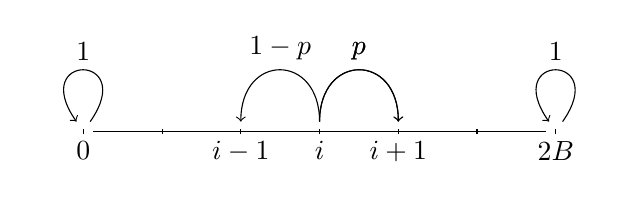
\begin{tikzpicture}
\foreach \x in {0,1,2,3,4,5,6}
	\draw (\x cm,-1pt) -- (\x cm, 1pt);
\node (null) at (0,0) {}; \draw (null) node[anchor=north] {$0$};
\node (a) at (2,0) {}; \draw (a) node [anchor=north] {$i-1$};
\node (b) at (3,0) {}; \draw (b) node [anchor=north] {$i$};
\node (c) at (4,0) {}; \draw (c) node [anchor=north] {$i+1$};
\node (zb) at (6,0) {}; \draw (zb) node [anchor=north] {$2B$};
\draw (null) -- (zb);
\draw [->] (b) .. controls +(up:1cm) and +(up:1cm) .. node [anchor=south] {$1-p$}  (a);
\draw [->] (b) .. controls +(up:1cm) and +(up:1cm) .. node [anchor=south] {$p$}  (c);
\draw [->] (b) .. controls +(up:1cm) and +(up:1cm) .. node [anchor=south] {$p$}  (c);
\draw [->] (null) .. controls +(0.7,1) and +(-0.7,1) .. node [anchor=south] {$1$}  (null);
\draw [->] (zb) .. controls +(0.7,1) and +(-0.7,1) .. node [anchor=south] {$1$}  (zb);
\end{tikzpicture}
\end{center}
\end{beispiel}

\begin{beispiel}[Wartesystem]
Zu jedem Zeitpunkt $n=0,1,\ldots$ können maximal $m$ Kunden bedient werden. $Y_n$ sei die Anzahl der zufällig im Zeitintervall $(n-1,n]$ eintreffenden Kunden und sei u.i.v.

Sei $X_n$ die Anzahl der zur Zeit $n$ wartenden Kunden, $S=\MdN_0$. Es gilt $X_0 = c$ und $X_n = (X_{n-1}-m)^+ + Y_n$. Also ist $(X_n)$ eine Markov-Kette mit Übergangsmatrix $P=(p_{ij})$ und $p_{ij} = P(Y_n = j-(i-m)^+)$, $i,j\in \MdN_0$.
\end{beispiel}

\begin{definition}
Sei $P$ eine stochastische $S\times S$-Matrix. Dann heißen die Elemente $p_{ij}^{(n)}$ von $P^n$ die $n$-Schritt-Übergangswahrscheinlichkeiten zu $P$. Wir definieren $P^0=E$, also $p^{(0)}_{ij}= \delta_{ij}$.
\end{definition}

\begin{satz}
Sei $(X_n)$ eine Markov-Kette mit Übergangsmatrix $P$. Dann gilt:
\begin{enuma}
\item $P(X_{n+m} = j\mid X_m = i) = p_{ij}^{(n)}$ für alle $i,j\in S$, $m,n\in\MdN_0$ mit $P(X_m=i)>0$.
\item $P(X_n = j) = \sum_{i\in S} P(X_0=i)p_{ij}^{(n)}$, $j\in S$, $n\in\MdN$.
\end{enuma}
\end{satz}

\begin{beweis}
\begin{enuma}
\item 
\begin{align*}
P(X_{n+m} =i_{n+m} , X_m=i_m) &= \sum_{i_{m+1},\ldots,i_{n+m-1}\in S} P(X_m = i_m) \prod_{k=m}^{m+n-1} p_{i_ki_{k+1}} \\
&= P(X_m = i_m) p_{i_mi_{m+n}}^{(n)}
\end{align*}
\item 
\begin{align*}
P(X_n=j) &= \sum_{i\in S} P(X_n=j, X_0=i) \\
&= \sum_{i\in S} P(X_n = j \mid X_0 = i)\cdot P(X_0 = i) \\
&= \sum_{i\in S} P(X_0 = i) p_{ij}^{(n)}
\end{align*}
\end{enuma}
\end{beweis}

\begin{bemerkung}
\begin{enumi}
\item Wegen $P^{n+m}  = P^n \cdot P^m$ gilt: 
\[
p_{ij}^{(n+m)}  = \sum_{k\in S} p_{ik}^{(n)}p_{kj}^{(m)} \text{ für } i,j\in S
\]
Dies ist die „Chapman-Kolmogorov-Gleichung“\index{Chapman-Kolmogorov-Gleichung!zeitdiskret}.
\item Ist $X_0 \sim \nu$, so gilt $X_n \sim \nu\cdot P^n$.
\end{enumi}
\end{bemerkung}

\begin{satz}[Existenzsatz für Markov-Ketten]
Sei $\nu$ ein Wahrscheinlichkeitsmaß auf $S$ und $P$ eine stochastische $S\times S$-Matrix. Sei $X_n$ die $n$-te Projektion auf $\Omega \da S^{\MdN_0}$, also $X_n : \Omega\to S$, $n\in\MdN_0$ mit $X_n(\omega) = X_n( (i_0,i_1,\ldots) ) = i_n$.

Dann existiert ein Wahrscheinlichkeitsmaß $P$ auf $\cF = \oplus_{n=0}^\infty \mathcal P (S)$, sodass $(X_n)$ eine Markov-Kette mit Übergangsmatrix $P$ und Startverteilung $\nu$ ist, d.h:
\begin{itemize}
\item $P(X_0 = i_0)= \nu(i_0)$, $i_0\in S$
\item $P(X_{n+1} = j \mid X_n= i) = p_{ij}$, $i,j\in S$, $P(X_n=i)>0$.
\end{itemize}
\end{satz}

\begin{beweis}
Satz von Ionescu-Tulcea über die Fortsetzung von Maßen und die Existenz zufälliger Folgen.
\end{beweis}

\section{Klassifikation von Zuständen, Rekurrenz und Transienz}

In diesem Paragraphen widmen wir uns Fragestellungen wie diesen:
Welche Zustände in $S$ werden von der Markov-Kette mit Sicherheit besucht und welche nicht? Wenn sie besucht werden, wie oft? 

\begin{definition}
Sei $(X_n)$ eine Markov-Kette mit Übergangsmatrix $P=(p_{ij})$.
\begin{enuma}
\item $i\in S$ \emph{führt nach} $j\in S$ (kurz $i\rightsquigarrow j$)\index{$\rightsquigarrow$}, falls es ein $n\in \MdN$ gibt mit $p_{ij}^{(n)}>0$.

\item $i\in S$ \emph{kommuniziert mit} $j\in S$ (kurz $i\leftrightarrow j)$\index{$\leftrightarrow$} falls sowohl $i\rightsquigarrow j$ als auch $j\rightsquigarrow i$ gilt.
\end{enuma}
\end{definition}

\begin{bemerkung}
Für $i,j\in S$ sei $i\sim j$ definiert als $(i\leftrightarrow j) \vee (i=j)$. Diese Relation ist eine Äquivalenzrelation auf $S$, da sie reflexiv, symmetrisch und transitiv ist.

Dies liefert uns eine Partition von $S$ mit den Äquivalenzklassen $K(i) \da \{j\in S \mid i\sim j\}$. Die Äquivalenzklasse $K(i)$ enthält $i$ selbst und die mit $i$ kommunizierenden Zustände.
\end{bemerkung}

\begin{definition}
Sei $(X_n)$ eine Markov-Kette mit Übergangsmatrix $P=(p_{ij})$.
\begin{enuma}
\item $J\subset S$ heißt \emph{abgeschlossen}\index{abgeschlossene Zustandsmenge}, wenn es keine zwei Zustände $j\in J$ und $i\in S\setminus J$ gibt mit $j\rightsquigarrow i$.
\item Die Markov-Kette $(X_n)$ beziehungsweise die Übergangsmatrix $P$ heißen \emph{irreduzibel}\index{irreduzibel}, falls $S$ nur aus einer Klasse besteht, also für alle $i,j\in S$, $i\ne j$, gilt $i\leftrightarrow j$.
\end{enuma}
\end{definition}

\begin{beispiel}
\emph{Skizze, hier ausgelassen}
\end{beispiel}

\begin{beispiel}[Ruinspiel]
$\mbox{}$
\begin{center}
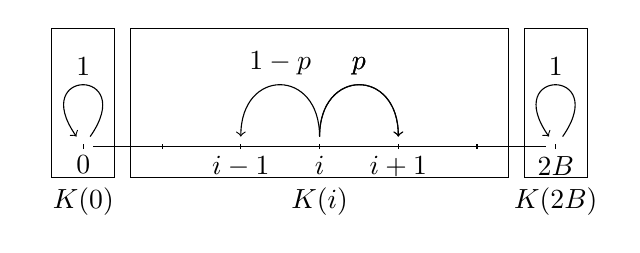
\begin{tikzpicture}
\foreach \x in {0,1,2,3,4,5,6}
	\draw (\x cm,-1pt) -- (\x cm, 1pt);
\node (null) at (0,0) {}; \draw (null) node[anchor=north] {$0$};
\node (a) at (2,0) {}; \draw (a) node [anchor=north] {$i-1$};
\node (b) at (3,0) {}; \draw (b) node [anchor=north] {$i$};
\node (c) at (4,0) {}; \draw (c) node [anchor=north] {$i+1$};
\node (zb) at (6,0) {}; \draw (zb) node [anchor=north] {$2B$};
\draw (null) -- (zb);
\draw [->] (b) .. controls +(up:1cm) and +(up:1cm) .. node [anchor=south] {$1-p$}  (a);
\draw [->] (b) .. controls +(up:1cm) and +(up:1cm) .. node [anchor=south] {$p$}  (c);
\draw [->] (b) .. controls +(up:1cm) and +(up:1cm) .. node [anchor=south] {$p$}  (c);
\draw [->] (null) .. controls +(0.7,1) and +(-0.7,1) .. node [anchor=south] {$1$}  (null);
\draw [->] (zb) .. controls +(0.7,1) and +(-0.7,1) .. node [anchor=south] {$1$}  (zb);
\draw (-0.4,-0.4) rectangle (0.4,1.5);
\draw (0,-0.4) node [anchor=north] {$K(0)$};
\draw (0.6,-0.4) rectangle (5.4,1.5);
\draw (3,-0.4) node [anchor=north] {$K(i)$};
\draw (5.6,-0.4) rectangle (6.4,1.5);
\draw (6,-0.4) node [anchor=north] {$K(2B)$};
\end{tikzpicture}
\end{center}
\end{beispiel}

\begin{lemma}
$J\subset S$ ist genau dann abgeschlossen, wenn $(p_{ij},\, i,j\in J)$ stochastisch ist.
\end{lemma}
\begin{beweis}
„$\Longrightarrow$“: Klar. „$\Longleftarrow$“: Es gilt: $(p_{ij},\, i,j\in J)$ stochastisch $\iff$ $(p_{ij}^{(n)},\, i,j\in J)$ stochastisch für alle $n\in \MdN$.
\end{beweis}

\pagebreak[2]
Sei $(X_n)$ eine Markov-Kette mit Übergangsmatrix $P=(p_{ij})$. Es sei
\[
T_i \da \inf\{n\in\MdN\mid X_n =i\}
\]
die (zufällige) Ersteintrittszeit der Markov-Kette in den Zustand $i$.

Wir setzen dabei $\inf\emptyset \da \infty$. Weiter sei für $i,j\in S$, $n\in \MdN$:
\begin{align*}
f_{ij}^{(n)} &\da P(T_j=n\mid X_0=i) = P_i(T_j=n) \\
&=P(X_n=j,\, X_\nu\ne j \text{ für } 1 \le \nu < n\mid X_0=i) \\
f_{ij}^{(0)} &\da 0
\end{align*}

Offenbar ist $f_{ij}^{(1)} = p_{ij}$. Weiter definieren wir
\[
f_{ij}^{*} \da \sum_{n=0}^\infty f_{ij}^{(n)} = \sum_{n=0}^\infty P_i(T_j=n) = P_i(T_j<\infty) = P_i(\exists n\in \MdN: X_n=j)\in[0,1]
\]

\begin{definition}
Ein Zustand $i\in S$ heißt \emph{rekurrent}\index{rekurrent}, falls $f_{ii}^{*} = 1$ und \emph{transient}\index{transient} sonst. % Das sind ganz wichtige Begriffe.
\end{definition}

\begin{lemma}
\label{lem:2.2}Für alle $n\in\MdN$, $i,j\in S$ gilt:
\[
p_{ij}^{(n)} = \sum_{k=1}^n f_{ij}^{(k)} p_{jj}^{(n-k)}
\]
\end{lemma}

\begin{beweis}[Methode des ersten Besuches]
Unter Verwendung der Formel $P(AB\mid C) = P(B\mid C)\cdot P(A\mid BC)$ für Ereignisse $A,B,C$ zeigen wir:
\begin{align*}
p_{ij}^{(n)} &= P_i(X_n=j) = \sum_{k=1}^n P({X_n=j},\, {X_\mu\ne j,\, 1\le\mu<k,\, X_k = j}\mid {X_0=i}) \\
&= \sum_{k=1}^n P_i(X_\mu\ne j,\, 1\le\mu<k,\, X_k = j)\cdot\\
&\quad\quad\quad\quad \underbrace{P(X_n=j\mid X_0=i,\,X_\mu\ne j,\, 1\le\mu<k,\, X_k = j)}_{=P(X_n=j\mid  X_k=j)}\\
&=\sum_{k=1}^nf_{ij}^{(k)} p_{jj}^{(n-k)}
\end{align*}
\end{beweis}

\begin{satz}
\label{satz2.3}%
$i\in S$ ist rekurrent genau dann, wenn gilt:
\[
\sum_{n=0}^\infty p_{ii}^{(n)} = \infty
\]
\end{satz}

\begin{beweis}
Für $s\in(0,1)$ erhalten wir aus Lemma \ref{lem:2.2}:
\begin{align*}
\sum_{n=0}^\infty p_{ii}^{(n)} s^n &= 1 + \sum_{n=1}^\infty p_{ii}^{(n)} s^n = \\
&= 1 + \sum_{n=1}^\infty s^n\sum_{k=1}^n f_{ii}^{(k)}p_{ii}^{(n-k)} \\
&= 1 + \sum_{k=1}^\infty f_{ii}^{(k)} s^k \sum_{n=k}^\infty p_{ii}^{(n-k)} s^{n-k} \\
&= 1 + \sum_{k=1}^\infty f_{ii}^{(k)} s^k \sum_{n=0}^\infty p_{ii}^{(n)} s^{n} 
\end{align*}

Abkürzend schreiben wir $F(s)\da \sum_{k=1}^\infty f_{ii}^{(k)} s^k$ und $P(s)=\sum_{n=0}^\infty p_{ii}^{(n)} s^{n}$, also gilt \[P(s) = 1 + F(s)\cdot P(s).\]
Nun sei $s\to 1$ (monotone Konvergenz!), und wir erhalten
\[
P(1) = 1 + f_{ii}^*\cdot P(1).
\]
Es folgt: Ist $f_{ii}^* = 1$, so gilt $P(1) = 1 + P(1)$, also ist $P(1) = \sum_{n=0}^\infty p_{ii}^{(n)} = \infty$. Ist ansonsten $f_{ii}^{*}<1$, so gilt $P(1) = \frac1{1-f_{ii}^*} < \infty$.
\end{beweis}
%$p,P,\pi,\Pi, \mathcal P, \mathfrak P, \mathfrak p$

\begin{bemerkung}
Die im Satz \ref{satz2.3} auftretende Reihe kann wie folgt interpretiert werden:
\begin{align*}
\sum_{n=0}^\infty p_{ii}^{(n)}
= \sum_{n=0}^\infty E_i[1_{[X_n=i]}]
%= \sum_{n=0}^\infty E_i[1_{[X_n=i]}]
= E_i(\sum_{n=0}^\infty 1_{[X_n=i]})
\end{align*}
Sie bezeichnet also die erwartete Anzahl der Besuche des Zustandes $i\in S$.
\end{bemerkung}

\begin{satz}[Solidaritätsprinzip]
Ist ein Zustand $i\in S$ rekurrent (bzw. transient), so ist jeder Zustand in $K(i)$ rekurrent (bzw. transient).
\end{satz}

\begin{beweis}
Sei $i$ rekurrent und $j\in K(i)$, $j\ne i$, das heißt es gibt $n,m\in \MdN$, sodass $p_{ij}^{(m)}\cdot p_{ji}^{(n)}>0$.
Mit der Abschätzung
\begin{align*}
\sum_{k=0}^\infty p_{jj}^{(k)} 
&\ge \sum_{k=0}^\infty p_{jj}^{(m+n+k)} 
\ge \sum_{k=0}^\infty p_{ji}^{(n)} p_{ii}^{(k)} p_{ij}^{(m)}
= p_{ij}^{(m)} p_{ji}^{(n)} \sum_{k=0}^\infty p_{ii}^{(k)}
\end{align*}
und Satz \ref{satz2.3} ist $\sum_{k=0}^\infty p_{jj}^{(k)}=\infty$ und $j$ rekurrent.
\end{beweis}

\begin{bemerkung}
Ist $i\in S$ rekurrent (bzw. transient), so sagen wir $K(i)$ ist rekurrent (bzw. transient).

Ist $(X_n)$ irreduzibel und ein $i\in S$ ist rekurrent (bzw. transient), so sagen wir $(X_n)$ ist rekurrent (bzw. transient).
\end{bemerkung}

\begin{beispiel}[Irrfahrt auf den ganzen Zahlen, „Random Walk“]
\label{bsp2.3}
Es sei $X_n=\sum_{k=1}^n Y_k = X_{n-1}+Y_n$ und $X_0=0$, wobei $(Y_n)$ u.i.v. mit \[P(Y_n=1)=p = 1 - P (Y_n=-1) =1-q,\quad p\in (0,1)\] ist ($S=\MdZ$).

\begin{center}
\begin{tikzpicture}
\foreach \x in {0,1,2,3,4,5,6}
	\draw (\x cm,-1pt) -- (\x cm, 1pt);
%\node (null) at (0,0) {}; \draw (null) node[anchor=north] {$0$};
\node (a) at (2,0) {}; \draw (a) node [anchor=north] {$i-1$};
\node (b) at (3,0) {}; \draw (b) node [anchor=north] {$i$};
\node (c) at (4,0) {}; \draw (c) node [anchor=north] {$i+1$};
%\node (zb) at (6,0) {}; \draw (zb) node [anchor=north] {$2B$};
\draw (null) -- (zb);
\draw [->] (b) .. controls +(up:1cm) and +(up:1cm) .. node [anchor=south] {$q$}  (a);
\draw [->] (b) .. controls +(up:1cm) and +(up:1cm) .. node [anchor=south] {$p$}  (c);
\draw [->] (b) .. controls +(up:1cm) and +(up:1cm) .. node [anchor=south] {$p$}  (c);
%\draw [->] (null) .. controls +(0.7,1) and +(-0.7,1) .. node [anchor=south] {$1$}  (null);
%\draw [->] (zb) .. controls +(0.7,1) and +(-0.7,1) .. node [anchor=south] {$1$}  (zb);
\end{tikzpicture}
\end{center}
$(X_n)$ ist nach Konstruktion eine irreduzible Markov-Kette. Ist $(X_n)$ rekurrent oder transient?

Wir wenden Satz \ref{satz2.3} an und untersuchen o.B.d.A. $i=0$. Es gilt für alle $n\in \MdN_0$:
\begin{align*}
p_{00}^{(2n+1)} &= 0\\
p_{00}^{(2n)} &= p^nq^n \binom{2n}{n} = p^nq^n \frac{(2n)!}{(n!)^2}\\
\intertext{
Mit der Stirling-Formel ($n! \simeq (\frac n e )^n\cdot \sqrt{2\pi n}$) erhält man dann}
p_{00}^{(2n)} &\approx (pq)^n\cdot \frac{(\frac{2n}e)^{2n} \sqrt{4\pi n}}{(\frac ne) ^{2n} 2\pi n} = \frac{(4pq)^n}{\sqrt{\pi n}}.
\end{align*}

\paragraph{Fall 1} Ist $p=q=\frac12$, so ist $p_{00}^{(2n)} \approx \frac1{\sqrt{\pi n}}$, also ist $\sum_{n=0}^\infty p_{00}^{(2n)} = \infty$ und die Markov-Kette ist rekurrent.

\paragraph{Fall 2} Ist dagegen $p\ne q$, also $pq<\frac14$, so ist $\sum_{n=0}^\infty p_{00}^{(2n)} \le c\cdot\sum_{n=0}^\infty (4pq)^n < \infty$, also ist die Markov-Kette transient.
\end{beispiel}

\begin{bemerkung}
Betrachtet man die symmetrische Irrfahrt auf $\MdZ^d$, also $p_{ij}= \frac1{2d}$ für $\|i-j\|=1$, mit $\|\cdot\|$ der $l^1$-Norm und $i,j\in \MdZ^d$, so ist die Irrfahrt rekurrent für $d=1,2$ und transient sonst.
\end{bemerkung}

\begin{lemma}
Liegen $i$ und $j$ in der selben rekurrenten Klasse, so gilt $f^*_{ij} = f^*_{ji}= 1$.
\label{lem:2.5}
\end{lemma}

\begin{lemma}
Für alle $i,j\in S$ gilt: Wenn $j$ transient ist, dann gilt
\[
\sum_{n=0}^\infty p_{ij}^{(n)} < \infty
\]
Insbesondere ist 
\[
\lim_{n\to\infty} p_{ij}^{(n)} = 0.
\]
\label{lem:2.6}
\end{lemma}

\begin{beweis}
Summiere die Gleichung in Lemma \ref{lem:2.2} über alle $n$:
\begin{align*}
\sum_{n=0}^\infty p_{ij}^{(n)} &=
\delta_{ij} + \sum_{n=1}^\infty \sum_{k=1}^n f_{ij}^{(k)}p_{jj}^{(n-k)} \\
&= \delta_{ij} + \sum_{k=1}^\infty f_{ij}^{(k)} \sum_{n=k}^\infty p_{jj}^{(n-k)} \\
&= \delta_{ij} + f_{ij}^* \underbrace{\sum_{n=0}^\infty p_{jj}^{(n)}}_{<\infty\text{ da $j$ transient}}  <\infty
\end{align*}
\end{beweis}

\begin{satz}
Ist eine Klasse $K\subseteq S$ rekurrent, so ist $K$ abgeschlossen bzw. $(p_{ij},\, i,j\in K)$ ist stochastisch.
\end{satz}

\begin{beweis}
Wir zeigen: Ist $i\in K$ rekurrent und $i\rightsquigarrow j$, $i\ne j$, dann gilt $j\rightsquigarrow i$ und damit $j\in K$.

Angenommen, $j\rightsquigarrow i$ gelte nicht, also $p_{ji}^{(n)} = 0$ für alle $n\in \MdN$, und sei $N\in\MdN$ die kleinste Zahl mit $p_{ij}^{(N)} > 0$. Es gilt nun für alle $n\in \MdN$
\[
P_i(X_N=j,X_n=i)=0.
\]
Denn für $n>N$ gilt:
$P_i(X_N=j,X_n=i)=p_{ij}^{(N)} p_{ji}^{(n-N)} = 0$ und für $n<N$ gilt: $P_i(X_N=j,X_n=i)=p_{ii}^{(n)} p_{ij}^{(N-n)} = 0$, da $N-n<N$.

Also ist $P_i(T_i\le m,X_N=j) = \sum_{n=1}^m P_i(T_i=n,X_N=j) \le \sum_{n=1}^m P_i(X_n=i, X_N=j) = 0$ und damit 
\begin{align*}
\sum_{n=1}^m f_{ii}^{(n)} 
&= P_i(T_i\le m) \\
&= P_i(T_i\le m, X_N\ne j) \\
&\le P_i(X_N\ne j) \\
&=1-P_i(X_N=j) = 1-p_{ij}^{(N)}.
\end{align*}
Für $m\to\infty$ folgt dann
\begin{align*}
1=f_{ii}^* = \sum_{n=1}^\infty f_{ii}^{(n)}\le 1-p_{ij}^{(N)} < 1,
\end{align*}
was ein Widerspruch ist.
\end{beweis}

\begin{satz}
Ist die Klasse $K$ endlich und abgeschlossen, so ist $K$ rekurrent.\label{satz:2.8}
\end{satz}

\begin{beweis}
Da $(p_{ij},\,i,j\in K)$ stochastisch ist, folgt induktiv, dass $(p_{ij}^{(n)},\, i,j\in K)$ stochastisch für alle $n\in\MdN$ ist. Angenommen, $K$ wäre transient. Sei dann $j\in K$, dann ist nach Lemma \ref{lem:2.6} $p_{ij}^{(n)}\to 0$ für $n\to\infty$ und alle $i\in S$. Für $i\in K$ folgt also: $1=\sum_{j\in K} p_{ij}^{(n)} \to 0$ für $n\to\infty$. Widerspruch.
\end{beweis}

\begin{bemerkung}
Insbesondere gilt: Ist $S$ endlich und $P$ irreduzibel, so ist die Markov-Kette rekurrent.
\end{bemerkung}

\begin{beispiel}[Irrfahrt mit reflektierenden Grenzen]
Die Irrfahrt ist irreduzibel und rekurrent nach Satz \ref{satz:2.8}.
\end{beispiel}

\subsection*{Absorbtionswahrscheinlichkeiten}
Sei $(X_n)_{n\in\MdN}$ eine Markov-Kette mit Zustandsraum $S$ und Übergangsmatrix $P=(p_{ij})$. Aufgrund der bisherigen Ergebnisse können wir $S$ zerlegen in rekurrente Klassen $K_1,K_2,\ldots$ und eine Menge von transienten Zuständen $T$, also $S=T\cup K_1\cup K_2\cup\ldots$.

Es sei $\tau \da \inf\{n\ge 0 \mid X_n\notin T\}$  die Austrittszeit aus der Menge der transienten Zustände. Für $i\in T$, $k\in T^c$ interessiert uns $u_{ik}=P_i(X_\tau = k)$, vorausgesetzt $P_i(\tau <\infty)=1$.

Wir unterteilen $P=(p_{ij})$ in 
\[
P = 
\begin{pmatrix}
Q & R \\
0 & \tilde P
\end{pmatrix}
\]
wobei $Q$ die Einschränkung von $P$ auf die transienten Zustände ist, also $Q=(q_{ij})=(p_{ij}, i,j\in T)$.

\begin{satz}
\label{satz:2.9}Für $i\in T$, $j\in T^c$ gilt:
\[
u_{ij} = \sum_{k\in T} q_{ik}u_{kj} + p_{ij}.
\]
\end{satz}

\begin{beweis}
Sei $i\in T$, $j\in T^c$. 
\begin{align*}
u_{ij} &= P_i(X_\tau = j)\\
&= \sum_{k\in S} P_i(X_\tau  = j, X_1=k) \\
&= \underbrace{\sum_{k\in T} P_i(X_\tau = j, X_1=k)}_{\ad A} + \underbrace{\sum_{k\in T^c} P_i(X_\tau = j, X_1 = k)}_{=p_{ij}} \\
A &= \sum_{k\in T}\sum_{n\ge 2} P_i(\tau = n, X_n = j, X_1=k)\\
&= \sum_{k\in T}\sum_{n\ge 2} P_i(X_2\in T, \ldots, X_{n-1}\in T, X_n= j, X_1=k) \\
&= \sum_{k\in T}\sum_{n\ge 2} P_i(X_2\in T, \ldots, X_{n-1}\in T, X_n= j\mid  X_1=k) \cdot P_i(X_1=k) \\
&= \sum_{k\in T}\sum_{n\ge 2} p_{ik} P_k(X_1\in T,\ldots,X_{n-2}\in T, X_{n-1}=j) \\
&= \sum_{k\in T}\sum_{n\ge 2} p_{ik} P_k(\tau = n-1, X_\tau = j) \\
&= \sum_{k\in T} p_{ik} P_k(X_\tau = j) \\
&= \sum_{k\in T} p_{ik} u_{kj}
\end{align*}
Da für $i,k\in T$ gilt: $p_{ik}=q_{ik}$, folgt die Behauptung.
\end{beweis}

\begin{bemerkung}
Es sei $U=(u_{ij})_{i\in T, j\in T^c}$. Dann lässt sich Satz \ref{satz:2.9} schrieben als $U=QU+R$ bzw. $U-QU=R$, also $(I-Q)U=R$. Falls $I-Q$ invertierbar ist, ist $U=(I-Q)^{-1}R$
\end{bemerkung}

\section{Stationäre Verteilungen}

Sei $(X_n)$ eine Markov-Kette mit Übergangsmatrix $P$ und Startverteilung $\nu$.

Dann ist $X_n \sim \nu \cdot P^n$. Im Allgemeinen hängt diese Verteilung von $n$ ab. Es gibt aber spezielle Verteilungen
$\nu$, sodass die mit dieser Verteilung gestartete Kette zu jedem Zeitpunkt $n$ die selbe Verteilung $\nu$ besitzt. Man sagt dann,
die Kette ist \emph{im Gleichgewicht} bzw. \emph{stationär}.

\begin{definition}
  Eine Abbildung $\nu: S \rightarrow \MdR_{\geq 0}$ heißt \emph{Maß}.

  NB: Ein Maß $\nu$ definiert ein Maß $\mathcal{P}(S) \rightarrow \MdR_{\geq 0}, A \mapsto \sum_{a \in A} \nu(a) $ im gewöhnlichen Sinne.
  Falls $\sum_{a \in S} \nu(a) = 1$, so definiert es sogar eine Verteilung.
\end{definition}

\begin{definition}
  Sei $(X_n)$ eine Markov-Kette mit Übergangsmatrix $P = (p_{ij})$. Ein Maß $\nu$ heißt \emph{invariant}\index{invariantes Maß!zeitdiskret} für $P$, falls $\nu \cdot P = \nu$, d.h.
  falls gilt:
  \begin{align*}
    \sum_{i \in S} \nu(i) \cdot p_{ij} = \nu(j).
  \end{align*}
  Ist $\nu$ eine Verteilung und invariant, so nennt man $\nu$ auch \emph{stationäre Verteilung}\index{stationäre Verteilung!zeitdiskret} oder \emph{Gleichgewichtsverteilung}.
\end{definition}

\begin{bemerkung}
  a) Ist $S$ endlich, so kann jedes (nichtdegenerierte) invariante Maß zu einer stationären Verteilung normiert werden.

  b) Ist $\nu$ invariant, so gilt $\nu \cdot P^n = \nu$ ($n \in \MdN_0$).

  Ist $\nu$ eine stationäre Verteilung, so gilt
  \begin{align*}
    P_\nu(X_n = j) = \sum_{i \in S} v(i) \cdot p_{ij}^{(n)} = \nu(j),
  \end{align*}
  d.h. die mit $\nu$ gestartete Kette hat zu jedem Zeitpunkt die Verteilung $\nu$.

  c) Ist $P$ irreduzibel und $\nu \neq 0$ ein invariantes Maß, so ist $\nu(j) > 0$ für jedes $j\in S$.

  Denn: $\nu \neq 0$, also existiert $i_0 \in S$ mit $\nu(i_0) > 0$.
  Wegen der Irreduzibilität gibt es ferner für jedes $j \in S$ ein $n \in \MdN_0$ mit $p_{i_0j}^{(n)} > 0$. Zusammen:
  \begin{align*}
    \nu(j) = \sum_{i \in S} \nu(i) \cdot p_{ij}^{(n)} \geq \nu(i_0) p_{i_0j}^{(n)} > 0
  \end{align*}
\end{bemerkung}


Gibt es immer ein invariantes Maß bzw. eine stationäre Verteilung? Ist es eindeutig?

Im Folgenden sei $P$ irreduzibel. Wir definieren für ein beliebiges $k \in S$ das Maß $\gamma_k$ wie folgt:
\begin{align*}
  \gamma_k(i) := E_k[\sum_{n=1}^{T_k} 1_{[X_n = i]}]
\end{align*}


\begin{satz}
\label{satz3.1}
  Sei $(X_n)$ irreduzibel und rekurrent, $k \in S$. Dann gilt:
  \begin{enuma}
  \item $\gamma_k$ ist ein invariantes Maß
  \item $0 < \gamma_k < \infty$
  \item $\gamma_k$ ist das einzige invariante Maß mit $\gamma_k(k) = 1$ (d.h. $\gamma_k$ ist eindeutig bis auf Vielfache).
  \end{enuma}
\end{satz}

\begin{beweis}
\begin{enuma}
\item Zunächst gilt:
  \begin{align*}
      \gamma_k(i)
    &= E_k[\sum_{n=1}^{T_k} 1_{[X_n = i]}]
     = E_k[\sum_{n=1}^\infty 1_{[X_n = i, n \leq T_k]}]
     = \sum_{n=1}^\infty P_k(X_n = i, n \leq T_k)\\
    &= \sum_{n=1}^\infty \sum_{j \in S,j\neq k} P_k(X_n = i, X_{n-1} = j, n \leq T_k)
  \end{align*}
  Für $j \neq k$ erhält man
  \begin{align*}
      &P_k(X_n = i, X_{n-1} = j, n \leq T_k)\\
    = &P(X_n = i, X_{n-1} = j, X_{n-2} \neq k, \ldots, X_1 \neq k, X_0 = k) / P(X_0 = k)\\
    = &P(X_n = i \mid X_{n-1} = j, X_{n-2} \neq k, \ldots, X_1 \neq k, X_0 = k) \cdot P_k(X_{n-1} = j, X_{n-2} \neq k, \ldots, X_1 \neq k)\\
    = &p_{ji} \cdot P_k(X_{n-1} = j, n \leq T_k)
  \end{align*}
  Die so erhaltene Identität gilt auch für $j = k$ und es folgt
  \begin{align*}
    \gamma_k(i) &= \sum_{n=1}^\infty \sum_{j \in S} P_k(X_n = i, X_{n-1} = j, n \leq T_k)\\
                &= \sum_{n=1}^\infty \sum_{j \in S} p_{ji} \cdot P_k(X_{n-1} = j, n \leq T_k)\\
                &= \sum_{j \in S} p_{ji} \sum_{n=0}^\infty P_k(X_n = j, n+1 \leq T_k)\\
                &= \sum_{j \in S} p_{ji} E_k[\sum_{n=0}^{T_k-1} 1_{[X_n = j]}]\\
                &= \sum_{j \in S} p_{ji} E_k[\sum_{n=1}^{T_k} 1_{[X_n = j]}]
                 = \sum_{j \in S} \gamma_k(j) p_{ji}
  \end{align*}

\item
  Nach Bemerkung c) oben gilt $\gamma_k > 0$, denn $\gamma_k(k) = 1$. Wegen $\gamma_k = \gamma_k \cdot P^n$ folgt
  \begin{align*}
    1 = \gamma_k(k) \geq \gamma_k(j) \cdot p_{jk}^{(n)}
  \end{align*}
  für jedes $j \in S$. Es gibt allerdings mindestens ein $p_{jk}^{(n)} > 0$, denn die Markov-Kette ist irreduzibel; daran erkennt man
  $\gamma_k < \infty$.

\item 
  Sei $\lambda$ ein weiteres, invariantes Maß mit $\lambda(k)=1$. Es gilt also:
  \begin{align*}
    \lambda(j) &= \sum_{i \in S\setminus\{k\}} \lambda(i) \cdot p_{ij} + 1 \cdot p_{kj}\\
               &= \sum_{i \in S\setminus\{k\}} \left( \sum_{l \in S\setminus\{k\}} \lambda(l) \cdot p_{li} + p_{ki} \right) p_{ij} + p_{kj}\\
               &= \sum_{i,l \in S\setminus\{k\}} \lambda(l) \cdot p_{li} \cdot p_{ij} + \sum_{i \in S\setminus\{k\}} p_{ki} \cdot p_{ij} + p_{kj}\\
               &= \sum_{i,l \in S\setminus\{k\}} \lambda(l) \cdot p_{li} \cdot p_{ij} + P_k(X_2 = j, T_k \geq 2) + P_k(X_1 = j, T_k \geq 1)
  \end{align*}
  Iterativ erhalten wir für $n \in \MdN$:
  \begin{align*}
    \lambda(j) &= \sum_{i_0, i_1, \ldots, i_n \in S\setminus\{k\}} \lambda (i_n) \prod_{r=1}^n p_{i_ri_{r-1}} p_{i_0j} + \sum_{r=1}^{n+1} P_k(X_r = j, T_k \geq 1)\\
               &\geq \sum_{r=1}^{n+1} P_k(X_r = j, T_k \geq 1) = E_k[\sum_{r=1}^{\min(n+1,T_k)} 1_{[X_r = j]}] \towegen{n\to\infty} \gamma_k(j).
  \end{align*}
  Es ist also $\lambda - \gamma_k$ ebenfalls ein invariantes Maß mit $(\lambda - \gamma_k)(k) = 0$; nach Bemerkung c) folgt
  $\lambda - \gamma_k = 0$, d.h. $\lambda = \gamma_k$.
\end{enuma}

\end{beweis}

\begin{bemerkung}
\begin{enuma}
\item Ist $S$ endlich und $P$ irreduzibel, so folgt aus Satz \ref{satz3.1}, dass eine stationäre Verteilung existiert.
\item Ist $(X_n)$ irreduzibel und transient, so kann  keine stationäre Verteilung existieren, denn:

Angenommen es existiert eine stationäre Verteilung $\pi$. Dann ist
\begin{align*}
\pi(j) &= \sum_{i\in S} \pi(i) p_{ij}^{(n)}.
\end{align*}
Für $n\to\infty$ wird daraus (mit majorisierter Konvergenz und der bekannten Eigenschaft transienter Übergangswahrscheinlichkeiten):
\begin{align*}
\pi(j) &= \sum_{i\in S} \pi(i) \lim_{n\to\infty} p_{ij}^{(n)} \\
&= \sum_{i\in S} \pi(i) \cdot 0 \\
&= 0
\end{align*}
\end{enuma}

\end{bemerkung}

\begin{definition}
Für $i\in S$ sei
\begin{align*}
m_i \da E_i[T_i] &= \sum_{n=1}^\infty n \cdot P_i(T_i=n) + \infty \cdot (1-f_{ii}^*) \\
&= \sum_{n=1}^\infty  n\cdot f_{ii}^{(n)} + \infty \cdot (1-f_{ii}^*)
\end{align*}
die \emph{mittlere Rückkehrzeit}\index{mittlere Rückkehrzeit} des Zustands $i$.
\end{definition}

\begin{bemerkung}
Ist $j$ transient, so folgt $m_j=\infty$.
\end{bemerkung}

\begin{definition}
Ein Zustand $i\in S$ heißt \emph{positiv rekurrent}\index{positiv rekurrent}, falls $m_i<\infty$ und \emph{nullrekurrent}\index{nullrekurrent}, falls $i$ rekurrent und $m_i=\infty$ ist.
\end{definition}

\begin{bemerkung}
Jeder positiv rekurrente Zustand ist auch rekurrent.
\end{bemerkung}

\begin{satz}
\label{satz3.2}Sei $(X_n)$ eine irreduzible Markov-Kette. Die folgenden Aussagen sind äquivalent:
\begin{enumi}
\item Es existiert eine stationäre Verteilung.
\item Es gibt einen positiv rekurrenten Zustand $i\in S$.
\item Alle Zustände in $S$ sind positiv rekurrent.
\end{enumi}
Sind diese Bedingungen erfüllt, so ist die stationäre Verteilung eindeutig und durch \[\pi(i)=\frac 1 {m_i}\] gegeben.
\end{satz}

\begin{beweis}
\begin{enumerate}[(iii) $\implies$ (ii)]
\item[(iii) $\implies$ (ii)] $\checkmark$
\item[(ii) $\implies$ (i)] Sei $k\in S$ mit $m_k<\infty$, dann ist $(X_n)$ rekurrent und mit Satz \ref{satz3.1} ist $\gamma_k$ ein invariantes Maß. Dann gilt:
\begin{align*}
\sum_{j\in S} \gamma_k(j) 
&= \sum_{j\in S} E_k[ \sum_{n=1}^{T_k} 1_{[X_n=j]}] \\
&= E_k[\sum_{n=1}^{T_k} \sum_{j\in S} 1_{[X_n=j]}] \\
&= E_k[\sum_{n=1}^{T_k} 1] \\
&= E_k[T_k] = m_k <\infty
\end{align*}
also ist $\gamma_k$ normierbar.

\item[(i) $\implies$ (iii)] Sei $\pi$ eine stationäre Verteilung und $k\in S$. Insbesondere sind $\pi(j)>0$ für alle $j\in S$. Dann ist $\gamma \da \frac{\pi}{\pi(k)}$ ein invariantes Maß mit $\gamma(k)=1$.  Nach Satz \ref{satz3.1} c) folgt $\gamma = \gamma_k$. Beachte dass im Beweis von \ref{satz3.1} c) die Voraussetzung $(X_n)$ rekurrent nicht verwendet wurde.
Wie oben ist 
\[
m_k=\sum_{j\in S}\gamma_k(j) = \frac 1 {\pi(k)} \sum_{j\in S} \pi(j) = \frac1{\pi(k)} < \infty.\]

Da $k\in S$ beliebig ist, folgt die Behauptung (iii).

Außerdem ist gezeigt, dass $\pi(k)=\frac1{m_k}$.
\end{enumerate}
\end{beweis}
\begin{bemerkung}
\begin{enumi}
\item Es gilt also die folgende Trichotomie für irreduzible Markov-Ketten, das heißt eine irreduzible Markov-Kette gehört immer zu genau einem der folgenden Fälle:
\begin{itemize}
\item Die Markov-Kette ist transient, es gibt keine stationäre Verteilung.
\item Die Markov-Kette ist nullrekurrent, insbesondere gilt für alle $i,j\in S$:
\[P_i(T_j<\infty) = 1\text{ und }E_i[T_j]=\infty\]
und es gibt ein (bis auf Vielfache) eindeutiges invariantes Maß, aber keine stationäre Verteilung.
\item Die Markov-Kette ist positiv rekurrent, für alle $i,j\in S$ ist $E_i[T_j]<\infty$ und es gibt eine stationäre Verteilung.
\end{itemize}

\item Ist $S$ endlich und die Markov-Kette irreduzibel, so ist sie automatisch positiv rekurrent.

\item Ist $\pi$ eine stationäre Verteilung, so gilt:
\begin{align*}
\pi(i) = \frac{\gamma_k(i)}{\sum_{j\in S} \gamma_k(j)}
= \frac{E_k[\sum_{n=1}^{T_k} 1_{[X_n=i]}]}{E_k[T_k]}.
\end{align*}
$\pi(i)$ ist also der durchschnittliche Bruchteil der Zeit, den die Markov-Kette im Zustand $i$ verbringt, während sie einen Zyklus durchläuft.
\end{enumi}
\end{bemerkung}

\begin{beispiel}
Sei $S=\{1,2\}$. Die Übergangsmatrix $P$ sei gegeben durch 
\[
P=
\begin{pmatrix}
1-\alpha & \alpha \\
\beta & 1-\beta
\end{pmatrix}, \quad \alpha,\beta \in (0,1].
\]
Also ist die Markov-Kette irreduzibel und positiv rekurrent. Die stationäre Verteilung ist die Lösung des linearen Gleichungssystems
\[ \pi P = \pi\]
unter Berücksichtigung von $\pi \ge 0$ und $\pi(1) + \pi(2) = 1$,
also
\[
\pi(1) = \frac\beta{\alpha + \beta}, \quad \pi(2)=\frac{\alpha}{\alpha+\beta}.
\]
\end{beispiel}

\begin{beispiel}[Irrfahrt]
Siehe Beispiel \ref{bsp2.3}: Für $p\ne q$ ist die Markov-Kette transient. Existiert ein invariantes Maß? Ansatz:
\[
\gamma(j) = \sum_{i\in \MdZ} \gamma (i) p_{ij} = \gamma(j+1)\cdot q + \gamma(j-1)\cdot p
\]
\[
\implies \gamma(j+1) - \gamma(j) = \frac pq (\gamma(j) - \gamma(j-1))
\]
Also: $\gamma_1(j) = 1$  und $\gamma_2(j) = (\frac pq)^{j}$, $j\in \MdZ$, sind verschiedene invariante Maße.

Ist $p=q=\frac 12$, so ist die Markov-Kette rekurrent. Ist sie nullrekurrent oder positiv rekurrent? Es gibt keine stationäre Verteilung (siehe oben), die Markov-Kette ist also nullrekurrent.
\end{beispiel}

\begin{beispiel}[Geburts- und Todesprozess in diskreter Zeit]
\label{bsp:3.3}Es sei $(X_n)$ eine Markov-Kette mit $S=\MdN_0$ und Übergangsmatrix 
\[
P = 
\begin{pmatrix}
p_{00} & p_{01} & 0 & \cdots \\
p_{10} & p_{11} & p_{12} & 0 & \cdots \\
0 & p_{21} & p_{22} & p_{23} & \ddots \\
\vdots & 0 & p_{32} & p_{33}  & \ddots \\
 & \vdots &\ddots & \ddots & \ddots  & 
 \end{pmatrix}
\]
mit $p_{01}>0$, $p_{i,i+1}>0$, $p_{i,i-1}>0$ für alle $i\ge 1$, also ist $(X_n)$ irreduzibel. Wann ist $(X_n)$ positiv rekurrent? 

Der Ansatz $\pi P=\pi$ liefert:
\begin{align*}
\pi(0) &= p_{00} \cdot \pi(0) + p_{10}\cdot \pi(1) \\
\pi(i) &= p_{i-1,i}\cdot \pi(i-1) + p_{ii}\cdot \pi(i) + p_{i+1,i}\cdot\pi(i+1) \\
\iff p_{i,i-1}\cdot \pi(i) + p_{i,i+1} \pi(i) &= p_{i-1,i}\cdot \pi(i-1) + p_{i+1,i} \cdot \pi(i+1) \\
\iff p_{i+1,i}\cdot \pi(i+1) - p_{i,i+1}\cdot \pi(i) &= p_{i,i-1}\cdot \pi(i) - p_{i-1,i}\cdot \pi(i-1) \\
&= \ldots = p_{10}\cdot\pi(1) - p_{01}\cdot\pi(0) \\
\intertext{Aus der ersten Gleichung folgt $p_{01}\cdot\pi(0) = p_{10}\cdot\pi(1)$ und damit:}
p_{i+1,i}\cdot \pi(i+1) - p_{i,i+1}\cdot \pi(i) &= 0 \\
\implies \pi(i+1) &= \frac{p_{i,i+1}}{p_{i+1,i}} \pi(i) \\
&= \ldots = \pi(0) \cdot \prod_{k=0}^i \frac{p_{k,k+1}}{p_{k+1,k}}.
\end{align*}
Für $\pi(0)>0$ erhält man ein invariantes Maß. $(X_n)$ ist positiv rekurrent, falls 
\[
\sum_{i=1}^\infty \prod_{k=0}^i \frac{p_{k,k+1}}{p_{k+1,k}} < \infty.
\]
Im Spezialfall $p_{k,k+1}=p$, $p_{k,k-1}=q=1-p$, $k\ge 1$ und $p_{01} = p$, $p_{00}=1-p$ gilt
\[
\text{$(X_n)$ ist positiv rekurrent} \iff \sum_{i=1}^\infty \left(\frac pq\right)^{i+1} < \infty \iff p<q.
\]

\end{beispiel}

\section{Konvergenz gegen die stationäre Verteilung}

Sei $(X_n)$ eine Markov-Kette mit Übergangsmatrix $P$. Wir nehmen an, dass $(X_n)$ bzw. $P$ aperiodisch ist, das heißt: Für alle Zustände $i\in S$ gilt: 
\[
d_i \da \operatorname{ggT}\{n\in \MdN \mid p_{ii}^{(n)}>0 \} = 1
\]

\begin{lemma}
\label{lem4.1}
$P$ ist genau dann irreduzibel und aperiodisch, wenn für alle $i,j\in S$ eine Zahl $n_0\in\MdN$ existiert, sodass für alle $n\ge n_0$ gilt: $p_{ij}^{(n)}>0$.
\end{lemma}

(ohne Beweis)

\begin{satz}[Konvergenzsatz]
Es sei $(X_n)$ irreduzibel, aperiodisch und positiv rekurrent mit stationärer Verteilung $\pi$. Dann gilt für alle $i,j\in S$:
\[
\lim_{n\to\infty} p_{ij}^{(n)} = \pi(j) = \frac1{m_j}
\]
\end{satz}

\begin{beweis}
Wir benutzen ein sogenanntes ``Kopplungsargument''.

(1) Sei $(Y_n)$ eine weitere Markov-Kette, unabhängig von $(X_n)$ mit gleicher Übergangsmatrix und Startverteilung $\pi$, also $Y_n\sim \pi$ für alle $n\in \MdN$. Es sei
\[
T\da \inf\{n\in \MdN \mid X_n = Y_n\}
\]
die Treffzeit der Markov-Kette. Wir zeigen zunächst: $P(T<\infty) = 1$.

Offenbar ist $(X_n,Y_n)_{n\in\MdN_0}$ eine Markov-Kette auf $S^2$ mit Übergangsmatrix $\hat P=(\hat p_{(ij)(kl)})$, wobei $\hat p_{(ij)(kl)} = p_{ik}\cdot p_{jl}$. Weiter ist $\hat p_{(ij)(kl)}^{(n)} = p_{ik}^{(n)} \cdot p_{jl}^{(n)}$ und mit Lemma \ref{lem4.1}: Die Kette $(X_n,Y_n)$ ist irreduzibel und aperiodisch. Man kann nachrechnen:
\[
\hat \pi (i,j) \da \pi(i)\cdot\pi(j)
\]
ist eine stationäre Verteilung für $(X_n,Y_n)$, also ist sie nach Satz \ref{satz3.2} positiv rekurrent.

Sei $X_0=i$. Die Startverteilung $\hat \nu$ von $(X_n,Y_n)$ gegeben durch $\hat \nu (k,l) = \delta_i(k) \cdot\pi(l)$. Für $b\in S$ sei 
\[
T_{(b,b)} \da \inf\{n\in\MdN \mid (X_n,Y_n) = (b,b) \}.
\]
Offenbar ist $T\le T_{(b,b)}$ und $P_{\hat \nu}(T_{(b,b)}<\infty)=1$. Daraus folgt, dass $P_{\hat \nu}(T<\infty)=1$.


(2) Betrachte $(Z_n)_{n\in\MdN_0}$ definiert durch
\[
Z_n= 
\begin{cases}
X_n, &\text{ für } n\le T \\
Y_n, &\text{ für } n>T.
\end{cases}
\]
Es ist $(Z_n)$ eine Markov-Kette mit Übergangsmatrix $P$ und $Z_0=i$, denn:

Nach Satz $\ref{satz1.1}$ genügt es zu zeigen, dass
\[\forall n\in\MdN\ \forall i,k\in S: P_{\hat\nu}(z_k=i_k,\, 0\le k\le n) = \delta_i(i_0) \prod_{k=0}^{n-1}p_{i_k}p_{i_{k+1}}\]
Es gilt
\begin{align*}
&\quad P_{\hat \nu}(Z_k=i_k,\,0\le k\le n)\\
&= \sum_{r=0}^n P_{\hat \nu}(Z_k=i_k,\, 0\le k\le n,\, T=r)\\
&\quad + P_{\hat \nu}(Z_k = i_k,\, 0\le k \le n,\, T>n) \\
&= \sum_{r=0}^n \underbrace{P(X_k = i_k,\, 0\le k\le r,\, Y_k=i_k,\, r+1\le k\le n,\, Y_0\ne i_0,\ldots, Y_{r-1}\ne i_{r-1},\, Y_r=i_r)}_{\ad \text{I}} \\
&\quad + \underbrace{P_{\hat \nu}(X_k = i_k, \, 0\le k\le n,\, Y_0\ne i_0,\ldots,Y_n\ne i_n)}_{\ad \text{II}}
\end{align*}
mit
\begin{align*}
  \text{I} &= P_{\hat \nu}(X_k = i_k, 0 \leq k \leq r) \cdot P_{\hat \nu}(Y_k = i_k, r+1 \leq k \leq n | Y_0 \neq i_0, \ldots, Y_{r-1} \neq i_{r-1}, Y_r = i_r) \cdot\\
           &~~~~ P_{\hat \nu}(Y_0 \neq i_0, \ldots, Y_{r-1} \neq i_{r-1}, Y_r = i_r)\\
           &= \delta_i(i_0) \cdot \prod_{k=0}^{r-1} p_{i_k,i_{k+1}} \cdot \prod_{k=r}^{n-1} p_{i_k,i_{k+1}} \cdot P_{\hat \nu}(Y_0 \neq i_0, \ldots, Y_{r-1} \neq i_{r-1}, Y_r = i_r)\\
           &= \delta_i(i_0) \cdot \prod_{k=0}^{n-1} p_{i_k,i_{k+1}} \cdot P_{\hat \nu}(Y_0 \neq i_0, \ldots, Y_{r-1} \neq i_{r-1}, Y_r = i_r),\\
  \text{II} &= \ldots = \delta_i(i_0) \cdot \prod_{k=0}^{n-1} p_{i_k,i_{k+1}} \cdot P_{\hat \nu}(Y_0 \neq i_0, \ldots, Y_{n-1} \neq i_{n-1}, Y_n \neq i_n)
\end{align*}
Tatsächlich gilt also
\begin{align*}
  P_{\hat \nu}(Z_k=i_k, 0 \leq k \leq n) = \delta_i(i_0) \cdot \prod_{k=0}^{n-1} p_{i_k,i_{k+1}}
\end{align*}

(3) Es gilt nun
\begin{align*}
    &p_{i,j}^{(n)} = P_{\hat \nu}(Z_n = j) = P_{\hat \nu}(Z_n = j, T \leq n) + P_{\hat \nu}(Z_n = j, T > n)\\
    &\pi(j) = P_{\hat \nu}(Y_n = j) = \underbrace{P_{\hat \nu}(Y_n = j, T \leq n)}_{= P_{\hat \nu}(Z_n = j, T \leq n)} + P_{\hat \nu}(Y_n = j, T > n)\\
  \Rightarrow \quad &|p_{i,j}^{(n)} - \pi(j)| \leq 2 \cdot P_{\hat \nu}(\underbrace{T > n}_{\downarrow \{T = \infty\}}) \longrightarrow 0
\end{align*}
\end{beweis}

\begin{satz}
  Seien $i$, $j \in S$ Zustände sowie $d_j$ die Periode von $j$. Dann gilt:
  \begin{align*}
    \lim_{n \rightarrow \infty} p_{i,j}^{(n \cdot d_j + r)} = \frac{d_j}{m_j} \sum_{k=0}^\infty f_{i,j}^{(k \cdot d_j + r)} \qquad r=1,\ldots,d_j
  \end{align*}
  Speziell:
  \begin{enuma}
  \item Ist $j$ transient oder nullrekurrent (d.h. $m_j = \infty$), so gilt $p_{i,j}^{(n)} \longrightarrow 0$
  \item Ist $j$ aperiodisch (d.h. $d_j = 1$), so gilt $p_{i,j}^{(n)} \longrightarrow \frac{1}{m_j} f_{i,j}^*$
  \end{enuma}
\end{satz}


\section{Markov-Ketten und Martingale}

\begin{erinnerung}
  $(X_n)$ heißt \emph{Martingal}, falls
  \begin{enuma}
  \item $E|X_n| < \infty$
  \item $E[X_{n+1}|X_1,\ldots,X_n] = X_n$, bzw.
  \item[b')] $E[X_{n+1}|\cF_n] = X_n$, wobei $\cF_n := \sigma(X_1, \ldots, X_n)$ die \emph{natürliche Filtration} bezeichnet.
  \end{enuma}
\end{erinnerung}

\begin{erinnerung}
  Sei $(\Omega, \cF, P)$ W-Raum, $X$ Zufallsvariable mit $E|X| < \infty$, $\mathcal{G} \subseteq \cF$ Unter-$\sigma$-Algebra.
  $Z \da E[X|\mathcal{G}]$ heißt bedingter Erwartungswert von $X$ bzgl. $\mathcal{G}$, falls
  \begin{enuma}
  \item $Z$ ist $\mathcal{G}$-messbar
  \item $\int_A Z \cdot dP = \int_A X \cdot dP$ \quad $\forall A \in \mathcal{G}$
  \end{enuma}
\end{erinnerung}

Sei $(X_n)$ eine Markov-Kette auf dem Zustandsraum $S$ mit Übergangsmatrix $P$ sowie $\cF_n := \sigma(X_1,\ldots,X_n)$ die natürliche
Filtration. Weiter sei $h: S \rightarrow \MdR$ und $P: (S \rightarrow \MdR) \rightarrow (S \rightarrow \MdR)$ definiert durch
\begin{align*}
  (Ph)(i) := \sum_{j \in S} p_{i,j} \cdot h(j)
\end{align*}
NB: ``Ph'' macht Sinn im Sinne einer ``Matrix$\cdot$Vektor''-Multiplikation.


\begin{lemma}
  \label{lemma_5_1}
  Sei $h: S \rightarrow \MdR$ eine Funktion mit $\left\|P \left|h\right| \right\|_\infty < \infty$. Dann gilt:
  \begin{align*}
    (Ph)(X_n) = E[h(X_{n+1})|\cF_n]
  \end{align*}
\end{lemma}
\begin{beweis}
  Wir prüfen, dass $(Ph)(X_n)$ ein bedingter Erwartungswert von $h(X_{n+1})$ bzgl. $\cF_n$ ist.

  a) $(Ph)(X_n)$ ist $\cF_n$-messbar, denn $X_n$ ist $\cF_n$-messbar.

  b) Sei $A := \{X_0 = i_0, \ldots, X_n = i_n\} \in \cF_n$. Dann:
  \begin{align*}
      &\int_A (Ph)(X_n) \cdot dP = \int 1_A \cdot (Ph)(X_n) \cdot dP = \int 1_{\{X_0 = i_0, \ldots, X_n = i_n\}} (Ph)(i_n) \cdot dP\\
    = &(Ph)(i_n) \cdot P(A) = \sum_{j \in S} p_{i_n,j} \cdot h(j) \cdot P(X_0 = i_0) \cdot \prod_{k=0}^{n-1} p_{i_k,i_{k+1}}\\
    = &\sum_{j \in S} h(j) \cdot P(X_0 = i_0, \ldots, X_n = i_n, X_{n+1} = j) = \sum_{j \in S} \int_{A \cap \{X_{n+1} = j\}} h(X_{n+1}) \cdot dP\\
    = &\sum_{j \in S} \int_A 1_{\{X_{n+1} = j\}} h(X_{n+1}) \cdot dP \stackrel{LDC}{=} \int_A h(X_{n+1}) \cdot dP
  \end{align*}
  Da jedes $A \in \cF_n$ abzählbare Vereinigung solcher ``Elementarereignisse'' ist, folgt die Behauptung.
\end{beweis}

\begin{satzunddefinition}
  Seien $P$ eine Übergangsmatrix auf $S$ und $h: S \rightarrow \MdR$ eine Funktion mit $\left\|P \left|h\right| \right\|_\infty < \infty$. Gilt
  dann $Ph = h$, so nennen wir $h$ \emph{harmonisch}. Im Fall $Ph \geq h$ bzw. $Ph \leq h$ heißt $h$ \emph{sub-} bzw. \emph{superharmonisch}.

  Ist $(X_n)$ eine Markov-Kette mit Übergangsmatrix $P$ und $h$ [sub-/super-]harmonisch, so ist $(h(X_n))$ ein $(\cF_n)$-[Sub-/Super-]Martingal.
\end{satzunddefinition}
\begin{beweis}
  Nach Lemma \ref{lemma_5_1} gilt
  \begin{align*}
    E[h(X_{n+1})|\cF_n] = h(X_n) + (Ph - h)(X_n)
  \end{align*}
  $\leadsto$ Behauptung.
\end{beweis}

\begin{bemerkung}
Ist $h:S\to \mathbb R$ eine beschränkte Funktion, so wird durch
\begin{align*}
Z_n^h &\coloneqq h(X_n) - \sum_{k=1}^n (E[h(X_k)\mid \cF_{k-1}] - h(X_{k-1})) \\
&= h(X_n) - \sum_{k=1}^n (Ph-h)(X_{k-1})
\end{align*}
ein Martingal definiert, genannt Levi-Martingal\index{Levi-Martingal} zu $(X_n)$.
\end{bemerkung}

Die Markoveigenschaft lässt sich über Levi-Martingale charakterisieren:

\begin{satz}
Es sei $(X_n)_{n\in\mathbb N_0}$ ein stochastischer Prozess mit Werten in $S$ und natürlicher Filtration $(\cF_n)$, d.h. $\cF_n=\sigma(X_0,\ldots,X_n)$, und $P$ sei eine stochastische Matrix auf $S$. Ist dann für alle beschränkten $h:S\to \mathbb R$ der Prozess
\begin{align*}
Z_n^h\coloneqq h(X_n) - \sum_{k=1}^n (Ph-h)(X_{k-1})
\end{align*}
ein $(\cF_n)$-Martingal, so ist $X_n$ eine homogene Markov-Kette mit Übergangsmatrix $P$.
\end{satz}

\begin{beweis}
Aus $E[Z_{n+1}^h\mid \cF_n] = Z_n^h$ erhält man 
\begin{align*}
E[h(X_{n+1})\mid \cF_n] = (Ph)(X_n)
\end{align*}
bzw. 
\begin{align*}
\int_A h(X_{n+1})dP = \int_A (Ph)(X_n)dP \text{ für alle }A\in \cF_n
\end{align*}
Es sei $i_0,i_1,\ldots,i_{n+1}\in S$ und $A\coloneqq \{X_0 = i_0,\ldots,X_n=i_n\}$ und wir setzen $h\da 1_{\{i_{n+1}\}}$. Die linke Seite der letzten Gleichung ergibt dann 
\begin{align*}
\int_A h(X_{n+1})dP &= P(X_0=i_0,\ldots,X_n=i_n,X_{n+1}=i_{n+1})
\end{align*}
und die rechte Seite ergibt
\begin{align*}
\int_A (Ph)(X_n)dP &= \int_{\{X_0=i_0,\ldots,X_n=i_n\}} (Ph)(i_n)dP \\
&= \int_{\{X_0=i_0,\ldots,X_n=i_n\}} p_{i_ni_{n+1}}dP \\
&= p_{i_ni_{n+1}} \cdot P(X_0=i_0,\ldots,X_n=i_n).
\end{align*}
Durch Teilen der rechten Wahrscheinlichkeit erhält man
\begin{align*}
P(X_{n+1}=i_{n+1} \mid X_0=i_0,\ldots,X_n=i_n) = p_{i_ni_{n+1}}.
\end{align*}
\end{beweis}

\begin{bemerkung}
Es gilt: Ist $(X_n)_{n\in\mathbb N_0}$ ein nicht-negatives Supermartingal, so gibt es eine Zufallsvariable $X_\infty$ mit 
\[
\lim_{n\to\infty} X_n = X_\infty \quad P-\text{f.s.}
\]
\end{bemerkung}

\begin{beispiel}
Jedem Feld eines schachbrettartigen $N\times N$-Gitters wird eine von $L$ möglichen Farben zugewiesen. Diese Färbung wird mittels Zufallsexperimenten modifiziert: Eine Zelle wird gleichverteilt gewählt, daraufhin wird einer der vier Nachbarn (modulo $N$) zufällig gewählt und dessen Farbe dem zuerst gewählten Feld zugewiesen. Offensichtlich ist dies eine Markov-Kette, und die monochromen Zustände sind die absorbierenden.

\begin{center}
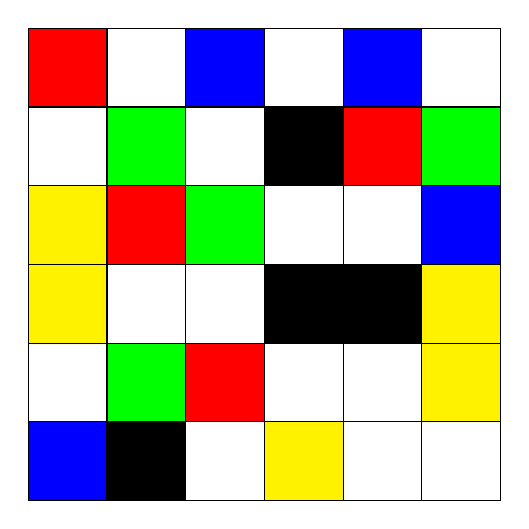
\begin{tikzpicture}
\draw[fill,color=blue] (0,0) rectangle +(1,1);
\draw[fill,color=blue] (4,2) rectangle +(1,1);
\draw[fill,color=blue] (4,5) rectangle +(1,1);
\draw[fill,color=blue] (5,3) rectangle +(1,1);
\draw[fill,color=blue] (2,5) rectangle +(1,1);
\draw[fill,color=black] (1,0) rectangle +(1,1);
\draw[fill,color=black] (3,2) rectangle +(1,1);
\draw[fill,color=black] (4,2) rectangle +(1,1);
\draw[fill,color=black] (3,4) rectangle +(1,1);
\draw[fill,color=yellow] (3,0) rectangle +(1,1);
\draw[fill,color=yellow] (0,2) rectangle +(1,1);
\draw[fill,color=yellow] (5,1) rectangle +(1,1);
\draw[fill,color=yellow] (5,2) rectangle +(1,1);
\draw[fill,color=yellow] (0,3) rectangle +(1,1);
\draw[fill,color=red] (1,3) rectangle +(1,1);
\draw[fill,color=red] (4,4) rectangle +(1,1);
\draw[fill,color=red] (0,5) rectangle +(1,1);
\draw[fill,color=red] (2,1) rectangle +(1,1);
\draw[fill,color=green] (1,1) rectangle +(1,1);
\draw[fill,color=green] (5,4) rectangle +(1,1);
\draw[fill,color=green] (1,4) rectangle +(1,1);
\draw[fill,color=green] (2,3) rectangle +(1,1);
\draw (0,0) grid (6,6);
\end{tikzpicture}
\end{center}

Formal seien $L,N\in \mathbb N$, $L,N\ge 2$. $I\coloneqq\{1,\ldots,N\}^2$, $S\coloneqq \{1,\ldots,L\}^I = \{f:I\to \{1,\ldots,L\}\}$. Sei $(X_n)$ die Markov-Kette in $S$, die die Zustandsfolge angibt.

Wie verhält sich die Folge für $n\to\infty$? Sei $l\in\{1,\ldots,L\}$ fest, und es sei $Y_n$ die Anzahl der Felder mit Farbe $l$ (zum Beispiel: blau) im Zustand $X_n$. Sei $(A,B)$ ein Nachbarpaar im Gitter. Wäre dies die Wahl in einem Zustandsübergang, so gelte: Ist $X_n(A)=X_n(B)$ oder $X_n(A)\ne l, X_n(B)\ne l$, so gilt auch $Y_{n+1}=Y_n$. Ist dagegen $X_n(A)=l$ und $X_n(B)\ne l$, so ist $Y_{n+1}=Y_n-1$. Ist letztlich $X_n(A)\ne l$ und $X_n(B) =l$, so ist $Y_{n+1}=Y_n+1$.

Die Wahrscheinlichkeit, erst $A$, dann $B$ zu wählen ist gleich der Wahrscheinlichkeit, erst $B$ und dann $A$ zu wählen. Damit ist
\[
E[Y_{n+1} \mid X_1,\ldots,X_n] = Y_n
\]
Sei $\cF_n \coloneqq \sigma(X_0,\ldots,X_n)$. Dann ist $(Y_n)_{n\in\mathbb N_0}$ ein $(\cF_n)$-Martingal. Nach der Bemerkung folgt: $Y_n\to Y_\infty$ für ein $n\to\infty$ $P$-fast-sicher. Da $(Y_n)$ ganzzahlig, ist $Y_n(\omega)$ konstant ab einem $n\ge n_0(\omega)$. Als Konstanten kommen nur $0$ und $N^2$ in Frage, denn für $k\in \{1,\ldots,N^2-1\}$ gilt
\begin{align*}
P(Y_{n+j} = k \mid Y_n = \ldots = Y_{n+j-1} = k) &\le 1 - \frac1{N^24} \\
\implies P(Y_n = \ldots = Y_{n+j} = k) &\le (1-\frac1{N^24})^j \\
\implies P(\underbrace{Y_m = k,\, \forall m\ge n}_{\eqqcolon A_n}) &= 0
\end{align*}
Es gilt $\{\omega \in \Omega \mid \exists n\ \forall m\ge n: Y_m(\omega)=k\} = \bigcup_{n=0}^\infty A_n$. Damit ist \[
P(\lim_{n\to\infty} Y_n=k) = P(\exists n\ \forall m\ge n: Y_n=k) \le \sum_{n=0}^\infty P(A_n) =0
\]
und wir folgern dass $P(Y_\infty \in \{0,N^2\}) = 1$.

Außerdem gilt noch, da $Y_n$ beschränkt sind:
\begin{align*}
EY_\infty = \lim_{n\to \infty} EY_n = EY_0
\end{align*}
Damit ist die Wahrscheinlichkeit, dass das Feld irgendwann komplett blau ist, gleich 
\begin{align*}
P(Y_\infty =N^2)=\frac 1{N^2} EY_\infty = \frac 1{N^2}EY_0 = \frac1{N^2}\#\{A\in I\mid X_0(A)=l\}.
\end{align*}

Anwendungen dieses Modells findet man in der Physik (Vielteilchensysteme), in der Biologie (Ausbreitung von Infektionen) oder in der Finanzmathematik (Kreditrisiken).
\end{beispiel}

\section{Die starke Markov-Eigenschaft}

Gegeben sei eine Markov-Kette $(X_n)_{n\in\mathbb N_0}$ mit Zustandsraum $S$ auf dem Wahrscheinlichkeitsraum $(\Omega = S_0^{\mathbb N_0}, \cF\da \otimes_{n=0}^\infty \mathcal P(S), P)$. Beachte, dass die Mengen
\begin{align*}
Z(i_0,i_1,\ldots,i_n) \coloneqq \{i_0\} \times \{i_1\} \times \cdots \times \{i_n\} \times S \times S \times \cdots
\end{align*}
für $n\in \mathbb N_0$, $i_0,\ldots i_n\in S$ ein durchschnittsstabiles Erzeugendensystem für $\cF$ bilden. Weiter sei $(\cF_n)_{n\in \mathbb N_0}$ mit $\cF_n=\sigma(X_0,\ldots,X_n)$ die natürliche Filtration von $(X_n)$.

$\tau:\Omega \to \mathbb N_0$ sei eine $(\cF_n)$-Stoppzeit\index{Stoppzeit}, das heißt $\{\tau \le n\} \in \cF_n$ und $P(\tau <\infty) = 1$. Die gestoppte Markov-Kette $X^\tau=(X_n^\tau)_{n\in\mathbb N_0}$ ist
\begin{align*}
X_n^\tau \da X_{\min(\tau,n)}
\end{align*}
für $n\in \mathbb N_0$ und $Y=(Y_n)_{n\in\mathbb N_0}$ definiert durch
\begin{align*}
Y_n \da X_{\tau + n}
\end{align*}
heißt der Post-$\tau$-Prozess.\index{Post-$\tau$-Prozess}

\begin{satz}[Starke Markov-Eigenschaft]
  \label{Satz6.1}
  Mit den oben eingeführten Bezeichnungen gilt:
  \begin{enuma}
  \item $Y$ ist eine Markov-Kette mit Übergangsmatrix $P$ 
    und Startverteilung $\nu$, wobei $X_\tau\backsim\nu$.
  \item $X^\tau$ und $Y$ sind unter $X_\tau$ bedingt unabhängig.
  \end{enuma}
\end{satz}

\begin{beweis}
  a.) Es gilt:
  \begin{align*}
    & P(Y_0=i_0,\dots,Y_n=i_n,Y_{n+1}=i_{n+1}) \\
    = & \sum_{k=0}^\infty P(\tau=k,X_k=i_0,\dots,X_{k+n+1}=i_{n+1}) \\
    = & \sum_{k=0}^\infty P(X_{k+n+1} = i_{n+1} \mid X_k=i_0,\dots,X_{k+n}=i_n,\tau=k) 
    \cdot P(X_k=i_0,\dots,X_{k+n}=i_n,\tau=k) \\
    = & p_{i_n i_{n+1}} \sum_{k=0}^\infty P(X_k=i_0,\dots,X_{k+n}=i_n,\tau=k) \\
    = & p_{i_n i_{n+1}} P(Y_0=i_0,\dots,Y_n=i_n) \implies \text{ Behauptung}.
  \end{align*}
  b.) Seien
  \begin{align*}
    & A:=Z(i_0,\dots,i_m)={i_0}\times\dots\times {i_m}\times S\times S \times\dots \\
    & B:=Z(j_0,\dots,j_n)
  \end{align*}
  dann gilt:
  \begin{align*}
    & P(X^\tau\in A,Y\in B,X_\tau =j) \\
    =& \sum_{k=0}^\infty P(\tau=k,X_{0\wedge k}=i_0,\dots,X_{m\wedge k}=i_m,
    X_k=j_0,\dots,X_{k+n}=j_n,X_k=j) \\
    =& \sum_{k=0}^\infty P(X_k=j_0,\dots,X_{k+n}=j_n\mid 
    X_{0\wedge k}=i_0,\dots,X_{m\wedge k}=i_m,X_k=j,\tau=k) \\
    & \quad \cdot P(X_{0\wedge k}=i_0,\dots,X_{m\wedge k}=i_m,X_k=j,\tau=k) \\
    =& P(X_0=j_0,\dots,X_n=j_n\mid X_0=j) \cdot P(X^\tau \in A, X_\tau=j) \\
    =& P(Y\in B\mid X_\tau=j) \cdot P(X^\tau\in A\mid X_\tau=j) \cdot P(X_\tau=j) 
  \end{align*}
  Teilen durch $P(X_\tau=j) \implies$ Behauptung.
\end{beweis}

\chapter{Markov-Ketten in stetiger Zeit}

\section{Ein wichtiger Spezialfall: der Poisson-Prozess}

Gegeben sei ein Wahrscheinlichkeitsraum $(\Omega,\cF,P)$.
Wir betrachten jetzt einen stochastischen Prozess $N=(N_t)_{t\geq 0}$
mit Zustandsraum $\mathbb{N}_0$, d.h. $(N_t)_{t\geq 0}$ ist eine Familie von
$(\cF,\mathcal{P}(\mathbb{N}_0))$-messbaren ZV, der bestimmte Ereignisse zählen soll
(z.B. Emission von Partikeln beim radioaktiven Zerfall, Ankünfte von Kunden in einem
Bediensystem, Schäden bei einer Versicherung). \\
Wir nehmen an, dass mindestens ein Ereignis eintritt und die Anzahl der Ereignisse in einem
kompakten Intervall soll endlich sein. \\
Wir stellen folgende Forderungen an $N$:
\begin{enumerate}[\hspace{1em}{(A}1)]
\item Alle Pfade $t \mapsto N(t,\omega)$ liegen in
\[
D_0:=\{f:[0,\infty)\longrightarrow\mathbb{N}_0\mid f(0)=0,f\uparrow,f \text{ stetig von rechts }\}
\]
%\emph{Hier fehlt ein Bild}
\item $(N_t)_{t\geq 0}$ hat unabhängige Zuwächse, d.h. für alle 
$0\leq t_0\leq t_1 \leq \dots \leq t_n, n\in \mathbb{N}$ sind die ZV
\[
N_{t_0},N_{t_1}-N_{t_0},\dots,N_{t_n}-N_{t_{n-1}}
\]
stochastisch unabhängig.
\item $(N_t)_{t\geq 0}$ hat stationäre Zuwächse, d.h. $\forall t>0$ hängt die Verteilung
von $N_{s+t}-N_s$ nicht von s ab.
\item Ereignisse treten einzeln auf, d.h. $P(N_h\geq2)=o(h)$ mit $h\downarrow 0$.
\end{enumerate}
\begin{bemerkung}
  Der stochastische Prozess kann als Zufallsgröße mit Werten in einem
  Funktionenraum aufgefasst werden, d.h.
  \[
  \Omega\ni\omega\mapsto N(\cdot,\omega)\in D_0
  \]
  Als $\sigma$-Algebra auf $D_0$ wählen wir 
  \[
  \borel(D_0):=\sigma(\{\pi_t:t\geq 0\})
  \]
  wobei $\pi_t:D_0\longrightarrow\mathbb{N}_0,f\mapsto f(t)$ die $t$-te Projektion ist. \\
  Es gilt: $N_t:\Omega\longrightarrow D_0$ ist $(\cF,\borel(D_0))$-messbar 
  $\Longleftrightarrow \pi_t \circ N_t:\Omega\longrightarrow\mathbb{N}_0$ sind 
  $(\cF,\mathcal P(\mathbb N_0))$-messbar $\forall t\geq0$. 
  (Stochastik II Übungsaufgabe 21) \\
  Die Mengen der Form
  \[
  A(t_1,\dots,t_n,i_1,\dots,i_n):=\{f\in D_0\mid f(t_j)-f(t_{j-1})=i_j \text{ für } j=1,\dots,n\}
  \]
  mit $0=:t_0\leq t_1\leq\dots\leq t_n\leq\infty,i_1,\dots,i_n\in\mathbb N$ 
  bilden ein durchschnittsstabiles Erzeugendensystem von $\borel(D_0)$.
\end{bemerkung}

\begin{satz}
  \label{satz:7.1}
  Es sei $(N_t)_{t\geq 0}$ ein stochastischer Prozess, der den Bedingungen (A1)-(A4) genügt.
  Dann hat $N$ mit Wahrscheinlichkeit $1$ nur Sprünge der Höhe $1$ und es existiert ein
  $\lambda>0$, so dass:
  \begin{enuma}
  \item $\forall s,t\geq 0$ ist $N_{s+t}-N_s$ Poisson-verteilt mit Parameter $\lambda t$.
  \item Die Zeiten zwischen aufeinanderfolgenden Sprüngen des Prozesses sind unabhängig und exponentialverteilt mit Parameter $\lambda$.
  \end{enuma}
\end{satz}


\begin{beweis} 
\textbf{Sprünge der Höhe 1:} Es ist also zu zeigen:
  \[
  P(N_s-N_{s-}\geq 2 \text{ für ein } s>0)=0
  \]
  wobei $N_{s-}$ der linksseitige Grenzwert ist. \\
  Für festes $t>0$ gilt:
  \begin{align*}
   & P(N_s-N_{s-}\geq 2 \text{ für ein } s\in (0,t]) \\
\leq \, & P(N_{\frac{kt}{n}}-N_{\frac{(k-1)t}{n}}\geq 2 \text{ für ein } k\in\{1,\dots,n\}) \\    
\leq \, & n\cdot P(N_{\frac{t}{n}}\geq 2)
  \end{align*}

(das letzte $\leq$ gilt wegen (A3)) \\
Aus (A4) folgt:
\[
\lim_{n\rightarrow\infty} \frac{P(N_{\frac{t}{n}}\geq 2)}{\frac{t}{n}}\cdot t=0
\]
Weiter gilt mit Stetigkeit des Wahrscheinlichkeitsmaßes:
\[
P(N_s-N_{s-}\geq 2 \text{ für ein } s>0)=
\lim_{t\rightarrow\infty}P(N_s-N_{s-}\geq 2 \text{ für ein } s\in (0,t])=0
\]

\textbf{a)} Betrachte dazu
\[
\Phi:[0,\infty) \to [0,1] \text{ mit }\Phi(t) \da P(N_t =0).
\]
Für alle $s,t>0$ folgt:
\begin{align*}
\Phi(s+t)
&= P(N_s = 0,N_{s+t} - N_s = 0) \\
 &= P(N_s=0) \cdot P(N_t=0) &\text{(nach (A3) und (A2))}\\
&= \Phi(s) \cdot \Phi(t)
\end{align*}
Daraus folgt, dass $\Phi(\frac kn) = (\Phi(\frac 1n))^k$ und $\Phi(1) = \Phi(\frac 1n + \cdots + \frac 1n) = (\Phi(\frac 1n))^n$ für $k,n\in \MdN$ gilt. Das heißt, dass $\Phi(\frac kn) = (\Phi(1))^{\frac kn}$.

Da $\Phi$ fallend ist folgt mit einem Einschachtelungsargument: 
\[
\Phi(t) = (\Phi(1))^t\text{ für alle } t >0
\]
Weiter ist $\Phi(1) \in (0,1)$, da $\Phi(1) \in[0,1]$ und falls $\Phi(1)=1$, dann wäre 
\[
P(N_t = 0 \text{ für alle } t\ge 0)= \lim_{t\to\infty} \Phi(t) = 1
\]
im Widerspruch zur Forderung, dass mindestens ein Ereignis eintritt, und wäre $\Phi(1) = 0$, dann gälte für alle $n\in \MdN$
\begin{align*}
P(N_1\ge n) 
&\ge P(N_{\frac kn} - N_{\frac {k-1}n} \ge 1 \text{ für } k =1,\ldots,n)\\
&= \Big(1-\Phi(\frac 1n)\Big) ^n &\text{((A2), (A3))} \\
&= 1
\end{align*}
im Widerspruch zur Forderung, dass in kompakten Intervallen nur endlich viele Ereignisse eintreten.

Sei jetzt 
\[
\lambda \da - \log \Phi(1).
\]
Es ist $0<\lambda <\infty$ und $P(N_t=0)= (\Phi(1))^t = e^{-\lambda t}$. Weiter sei $t>0$ und für $n\in \MdN$ definieren wir
\begin{align*}
X_{nk} &\da 1_{\MdN}\big(N_{\frac{kt}n} - N_{\frac{(k-1)t}n}\big)\\
&= 
\begin{cases}
1, &\text{falls mindestens ein Ereignis in $\big(\frac{kt}n, \frac{(k-1)t}n\big]$ eintritt}\\
0, &\text{sonst}
\end{cases}
\end{align*}
Wegen (A2) sind die $X_{n1},\ldots,X_{nn}$ unabhängig und wegen (A3) identisch verteilt mit $B(1,1-e^{-\lambda \frac tn})$. Dann gilt
\begin{align*}
\sum_{k=1}^n X_{nk} \sim B(n,1-e^{-\lambda \frac tn}) \tomit d \operatorname{Po}(\lambda t)
\end{align*}
da $n(1-e^{-\lambda \frac tn}) \tomit{n\to \infty} \lambda t$.

Aus (A4) folgt:
\begin{align*}
P(\sum_{k=1}^n X_{nk} \ne N_t) 
&= P(\bigcup_{k=1}^n\{N_{\frac {kt}n} - N_{ \frac{(k-1)t}n} \ge 2\})\\
&\le n \cdot P(N_{\frac tn} \ge 2) \tomit {n\to \infty} 0
\end{align*}
und damit haben wir gezeigt, dass
\[
N_t \sim \operatorname{Po}(\lambda t).
\]

\textbf{b)} Sei
\[
T_1 \da \inf \{t>0\mid N_t \ne 0\}
\]
der erste Sprungzeitpunkt. Wir erhalten
\begin{align*}
P(T_1 > t) = P(N_t = 0) = e^{-\lambda t}\text{ mit } t \ge 0
\end{align*} und damit
\[
T_1 \sim \operatorname{Exp}(\lambda).
\]
Die weiteren Aussagen werden später gezeigt.
\end{beweis}


\begin{bemerkung}
Der Prozess $N=(N_t)_{t\ge 0}$ in Satz \ref{satz:7.1} heißt \emph{Poisson-Prozess}\index{Poisson-Prozess} mit Parameter $\lambda$.
\end{bemerkung}

Die Bedingungen (A2) und (A3) können etwas „abstrakter“ gefasst werden: Für $u\ge 0$ definiere
\begin{align*}
S_u &: D_0 \to D_0,  & f &\mapsto f(\cdot\wedge u)\\
Z_u &: D_0 \to D_0,  & f &\mapsto f(u+\cdot)-f(u)
\end{align*}
wobei $(\cdot \wedge u)$ die Abbildung $v\mapsto \min (v,u)$ darstellt.

Beide Abbildungen sind $(\borel(D_0), \borel(D_0))$-messbar.

Wir können also auch stochastische Prozesse $S_u(N) = (N_{t\wedge u})_{t\ge 0}$ und $Z_u(N) = (N_{u+t} - N_u)_{t\ge 0}$ als Zufallsgröße mit Werten in $(D_0,\borel(D_0))$ auffassen.

Weiter gilt mit 
\[
A(t_1,\ldots,t_n;i_1,\ldots,i_n) \da \{f\in D_0\mid f(t_j) - f(t_{j-1}) = i_j\text{ für }j=1,\ldots,n\},
\]
wobei $0 \ad t_0\le t_1\le \cdots\le t_n < \infty$, $i_1,\ldots,i_n\in\MdN_0$, dass
\[
\{S_u(N) \in A(t_1,\ldots,t_n;i_1,\ldots,i_n)\} 
= \{ N_{t_1\wedge u}- N_{t_0\wedge u} = i_1,\ldots,N_{t_n\wedge u}- N_{t_{n-1}\wedge u} = i_n\}
\]
und
\[
\{Z_u(N) \in A(s_1,\ldots,s_l;j_1,\ldots,j_l)\} 
= \{ N_{u+s_1}- N_{u+s_0} = j_1,\ldots,N_{u+s_l}- N_{u+s_{l-1}} = j_l\} 
\]
Wegen (A2) folgt:
\begin{multline*}
P\big(S_u(N) \in A(t_1,\ldots,t_n;i_1,\ldots,i_n),\,
 Z_u(N) \in A(s_1,\ldots,s_l;j_1,\ldots,j_l)\big) \\
= P\big(S_u(N) \in A(t_1,\ldots,t_n;i_1,\ldots,i_n)\big) 
\cdot P\big(Z_u(N) \in A(s_1,\ldots,s_l;j_1,\ldots,j_l)\big) 
\end{multline*}
und daraus die Unahbhängigkeit der Prozesse $S_u(N)$ und $Z_u(N)$.

Analog folgt:
\[
P\big(Z_u(N) \in A(s_1,\ldots,s_l;j_1,\ldots,j_l)\big) 
= P\big( N \in A(s_1,\ldots,s_l;j_1,\ldots,j_l)\big)
\]
Also haben $Z_u(N)$ und $N$ dieselbe Verteilung.

Diese Aussagen können jetzt auf Stoppzeiten verallgemeinert werden. Es sei dazu $\cF_t \da \sigma(\{N_s, s\le t\})$ für $t\ge 0$ und $(\cF_t)_{t\ge 0}$ die natürliche Filtration.

\begin{definition}
Sei $\tau$ eine $(\cF_t)_{t\ge 0}$-Stoppzeit\index{Stoppzeit}, das heißt $\{\tau \le t \} \in \cF_t$. Der Prozess 
\[
S_\tau(N) = (N_{\tau \wedge t})_{t\ge 0}
\]
heißt \emph{Prä-$\tau$-Prozess}\index{Prä-$\tau$-Prozess} und der Prozess 
\[
Z_\tau(N) = (N_{\tau + t} - N_\tau)_{t \ge 0}
\]
heißt \emph{Post-$\tau$-Prozess}\index{Post-$\tau$-Prozess}.
\end{definition}

\begin{lemma}
\label{lem:7.2}
Ist $\tau$ eine endliche Stoppzeit, so sind die Prozesse $(N_{\tau \wedge t})_{t\ge 0}$ und $(N_{\tau + t}-N_\tau)_{t\ge 0}$ stochastisch unabhängig. Außerdem hat $(N_{\tau + t}-N_\tau)_{t\ge 0}$ dieselbe Verteilung wie $(N_t)_{t\ge 0}$.
\end{lemma}

\begin{beweis}
Zunächst nehmen wir an, dass $\tau$ Werte in $\mathbb Q_+$ annimmt. Für $0\le s_1\le\cdots\le s_k$, $0\le t_1\le \cdots\le t_l$ und beliebige $i_1,\ldots,i_k,j_1,\ldots,j_l\in \mathbb N_0$ gilt
\begin{align*}
C&\da P\big(S_\tau(N) \in \underbrace{A(s_1,\ldots,s_k;i_1,\ldots,s_k)}_{\ad A},\,
Z_\tau(N) \in \underbrace{A(t_1,\ldots,t_l;j_1,\ldots,j_l)}_{\ad B}
\big) \\
&= \sum_{u\in \mathbb Q_+} P(\tau = u,\, S_u(N)\in A,\, Z_u(N)\in B)\\
\intertext{Da $\{\tau = u \} \in \cF_u$ kann dieses Ereignis durch $S_u(N)$ ausgedrückt werden. Da $S_u(N)$ und $Z_u(N)$ unabhängig sind, folgt:
}
\cdots &= \sum_{u\in\mathbb Q_+} P(\tau = u, S_u(N)) \cdot \underbrace{P(Z_u(N)\in B)}_{= P(N\in B)} \\
&= P(N\in B) \cdot P(S_\tau(N) \in A)
\end{align*}
Im Fall $k=1,s_1=0,i_1=0$ folgt:
\begin{align*}
P(Z_\tau(N)\in B) = P(N\in B)
\end{align*}
also gilt $Z_\tau(N) \gleichnach{d} N$ und damit
\begin{align*}
P(S_\tau (N) \in A,\, Z_\tau(N)\in B) = P(Z_\tau (N) \in B) \cdot P(S_\tau(N)\in A)
\end{align*}
also sind $Z_\tau(N)$ und $S_\tau(N)$ unabhängig.

Weiter sei $\tau$ beliebig. Betrachte die Folge 
\[
\tau_n \da \frac{\lceil 2^n \tau \rceil}{2^n},\, n\in \mathbb N,
\]
für die $\tau_n\in \mathbb Q_+$ $P$-fast-sicher gilt und $\tau_n\to \tau$ für $n\to\infty$. Mit (A1) folgt für alle $t\ge 0$
\[
N_{\tau_n\wedge t} \tomit{n\to\infty} N_{\tau \wedge t},\quad N_{\tau_n+t}\tomit{n\to\infty}N_{\tau+t}
\]
$P$-fast-sicher und
\begin{align*}
P(S_\tau(N)\in A,\, Z_\tau(N)\in B) 
&= \lim_{n\to\infty} P(S_{\tau_n}(N)\in A,\, Z_{\tau_n}(N)\in B) \\
&= \lim_{n\to\infty} P(S_{\tau_n}(n)\in A) \cdot P(Z_{\tau_n}(N)\in B)\\
&= P(S_\tau(N)\in A)\cdot P(Z_\tau(N)\in B)
\end{align*}

Analog kann man die Aussage $Z_\tau(N)\gleichnach{d}N$ auf beliebige $\tau$ erweitern.
\end{beweis}

Damit können wir den Beweis von Satz $\ref{satz:7.1}$ abschließen:

Es seien
\begin{align*}
T_1 &\da \inf\{t>0\mid N_t\ne 0\} \\
S_1 &\da T_1 \\
S_k &\da \inf\{t>S_{k-1} \mid N_t \ne T_{t-}\},\ k=2,3,\ldots\\
T_k &\da S_k - S_{k-1},\ k=2,3,\dots
\end{align*}
Wir wissen bereits, dass $T_1 \sim \exp(\lambda)$. Induktiv nehmen wir an, dass $T_1,\ldots,T_k$ unabhängig und identisch exponential-verteilt seien. $\tau \da T_1 + \cdots + T_k = S_k$ ist eine Stoppzeit, da $\{\tau \le t\} = \{N_t \ge k\} \in \cF_t$. Da $P(\tau > t)= P(N_t < k) \to 0$ für $t\to\infty$ gilt, ist $\tau$ $P$-fast-sicher endlich.

$T_{k+1}$ ist die Zeit bis zum ersten Sprung im Post-$\tau$-Prozess. Nach Lemma $\ref{lem:7.2}$ ist $T_{k+1}\gleichnach{d} T_1\sim \exp(\lambda)$ und $T_{k+1}$ ist unabhängig von $S_\tau(N)$, also auch von $T_1,\ldots,T_k$.

\begin{beispiel}[Bedingte Gleichverteilungseigenschaft]
Es seien $K,X_1,X_2,\ldots$ unabhängige Zufallsvariablen mit $K\sim \operatorname{Po}(\lambda T)$, $T>0$, und $X_i\sim U(0,T)$.

Wir definieren\[
N_t \da \#\{1\le i \le K\mid X_i\le t\},\, t\ge 0.
\]
Es sei $0\ad t_0\le t_1 \le \cdots\le t_n=T$ eine Zerlegung des Intervals $[0,T]$. Betrachte für $i_1,\ldots,i_n\in \mathbb N_0$ das Ereignis
\[
A \da \{N_{t_1} - N_{t_0} = i_1,\ldots,N_{t_n}-N_{t_{n-1}} = i_n\}.
\]
Für $\omega \in A$ folgt $k \da K(\omega) = i_1+\cdots+ i_n$. Man erhält (siehe Definition der Multinomialverteilung, Henze, Stochastik I, S. 121)
\begin{align*}
P(N_{t_1} - N_{t_0}=i_1,\ldots,N_{t_n} - N_{t_{n-1}} = i_n) 
&= e^{-\lambda T}\frac{(\lambda T)^k}{k!}\cdot \frac{k!}{i_1!\cdots i_n!}\cdot\Big(\frac{t_1-t_0}{T}\Big)^{i_1}\cdots \Big(\frac{t_n-t_{n-1}}{T}\Big)^{i_n} \\
&= \prod_{l=1}^n \underbrace{e^{-\lambda(t_l-t_{l-1})} \frac{(\lambda (t_l - t_{l-1}))^{i_l}}{i_l!}}_{=P(M_l=i_l)}
\end{align*}
wobei $M_l\sim \operatorname{Po}(\lambda(t_l-t_{l-1}))$. Das zeigt: Die Zuwächse des Prozesses $\tilde N=(N_t)_{0\le t\le T}$ sind unabhängig und stationär und Poisson-verteilt mit Parameter $\lambda\cdot$Intervalllänge, und (A1), (A4) ist erfüllt, also ist $\tilde N$ ein bei $T$ gestoppter Poisson-Prozess.
\end{beispiel}

\begin{beispiel}[Das Inspektions-Paradoxon]
Es seien $X_1,X_2,\ldots$ unabhängig und identisch verteilte Zufallsvariablen mit $X_k\sim \exp(\lambda)$, welche die Lebensdauer von Glühbirnen modellieren.

Es sei $S_n \da \sum_{k=1}^n X_k$ der Zeitpunkt, an dem die $n$-te Birne kaputt geht und eine neue Birne eingesetzt wird, und $N_t$ die Anzahl der Erneuerungen bis zum Zeitpunkt $t$ und damit ein Poisson-Prozess mit Parameter $\lambda$.

In der Erneuerungstheorie interessiert man sich für 
\begin{align*}
V_t &\da S_{N_t+1}-t = \text{Restlebensdauer} \\
W_t &\da t- S_{N_t} = \text{Alter} \\
L_t &\da  W_t + V_t = \text{Gesamtlebensdauer}
\end{align*}
der zum Zeitpunkt $t$ in Gebrauch befindlichen Glühbirne.

Es ist $V_t \sim \exp(\lambda)$, da die Exponentialverteilung gedächtnislos ist. Die Variable $W_t$ kann höchstens $t$ sein, das heißt $P(W_t > s) = 0$ für $s>t$. Für $0\le s \le t$ gilt $P(W_t \ge s) = P(N_t-N_{t-s} = 0) = e^{-\lambda s}$. Damit ist
\begin{align*}
F_{W_t}(s) = 
\begin{cases}
1-e^{-\lambda s},& 0\le s \le t \\
1, & s\ge t.
\end{cases}
\end{align*}
Außerdem sind nach der starken Markoveigenschaft die Zufallsvariablen $W_t$ und $V_t$ unabhängig. $L_t$ ergibt sich als Faltung dieser Variablen. Die Dichte $f_{L_t}$ für $s\ge t$:
\begin{align*}
f_{L_t}(s) &= \int_0^s f_{V_t}(s-u)F_{W_t}(du) \\
&= \int_0^t \lambda e^{-\lambda(s-u)}\lambda e^{-\lambda} du + \lambda e^{-\lambda(s-t)}\cdot e^{-\lambda t} \\
&= \lambda (1+\lambda t)e^{-\lambda s}\\
\intertext{und für $s < t$:}
f_{L_t}(s) &= \int_0^s \lambda e^{-\lambda(s-u)}\lambda ^{-\lambda u}du \\
&= \lambda ^2 s e^{-\lambda s}
\end{align*}
Also ist $L_t$ \emph{nicht} $\exp(\lambda)$-verteilt! Für großes $t$ gilt
\[
EL_{t} \approx 2 EX_i=\frac 2 {\lambda}.
\]
Dieses Ergebnis lässt sich erklären: Inspiziert man zu einer zufälligen Zeit die aktuell leuchtende Glühbirne, so ist die Wahrscheinlichkeit, eine länger lebende zu erwischen, größer, als eine kurzlebige Birne anzutreffen.
\end{beispiel}

\section{Der allgemeine Fall im Schnelldurchgang}

\begin{definition}
Ein stochastischer Prozess $(X_t)_{t\ge 0}$ mit abzählbarem Zustandsraum $S$ heißt (homogene) Markov-Kette,\index{Markov-Kette!zeitstetig} falls gilt:
Für alle $n\in\mathbb N$ und $0\le t_0 < t_1 < \cdots < t_n$, $t,h>0$ und $i_k\in S$ mit $P(X_{t_k}=i_k,\, 0\le k\le n) > 0$:
\begin{align*}
P(X_{t_n+h}=i_{n+1} \mid X_{t_k}=i_k,\, 0\le k\le n) &= P(X_{t_n+h} = i_{n+1} \mid X_{t_n} = i_n) \\ 
&= P(X_{t+h} = i_{n+1} \mid X_t=i_n)
\end{align*}
\end{definition}

\begin{bemerkung}
Definieren wir für alle $i,j\in S$
\[
p_{ij}(t) \da P(X_t = j \mid X_0 = i)
\]
und die Matrix
\[
P(t) = \big(p_{ij}(t)\big)_{i,j\in S}
\]
so gelten analog zum diskreten Fall die Chapman-Kolmogorov-Gleichungen für alle $i,j\in S$, $s,t>0$:\index{Chapman-Kolmogorov-Gleichung!zeitstetig}
\[
p_{ij}(t+s) = \sum_{k\in S} p_{ik}(t) p_{kj}(s)
\]
Mit $P(0)=E$ wird $\{P(t): t\ge 0\}$ zu einer Halbgruppe von stochastischen Matrizen. Diese nennen wir \emph{Übergangsmatrizenfunktion}\index{Übergangsmatrizenfunktion}.

Falls zusätzlich für $i,j\in S$ 
\[
\lim_{t\downarrow 0} p_{ij}(t)=\delta_{ij}
\]
gilt, also $P(t)$ rechtsseitig stetig ist, dann heißt sie \emph{Standardübergangsmatrizenfunktion}\index{Standardübergangsmatrizenfunktion}.
\end{bemerkung}


\begin{satzunddefinition}
Sei $\{P(t): t\ge 0\}$ eine Standardübergangsmatrizenfunktion. Dann ist jedes $p_{ij}(t)$ in 0 rechtseitig differenzierbar, das heißt es existiert für alle $i,j\in S$
\[
q_{ij} \da \lim_{t\downarrow 0} \frac 1t (p_{ij}(t) - \delta_{ij}).
\]
Die Matrix $Q\da (q_{ij})$ heißt \emph{Intensitätsmatrix}\index{Intensitätsmatrix} oder \emph{infinitesimaler Erzeuger}\index{infinitesimaler Erzeuger} (Generator) zu $\{P(t): t\ge 0\}$.
\end{satzunddefinition}

\begin{beispiel}
Es sei $N=(N_t)_{t\ge 0}$ ein Poisson-Prozess mit Intensität $\lambda$. Dann gilt für $i_{n+1}\ge i_n$:
\begin{align*}
P(N_{t_{n+1}} = i_{n+1} \mid N_{t_0} = i_0 ,\ldots,N_{t_n}=i_n)
&= P(N_{t_{n+1}} - N_{t_n} = i_{n+1} - i_n)\\
&= e^{-\lambda (t_{n+1}-t_n)}\frac{(\lambda(t_{n+1}-t_n))^{i_{n+1}-i_n}}{(i_{n+1}-i_n)!}
\end{align*}
Also ist $N$ eine homogene Markov-Kette mit Übergangsmatrix
\[
p_{ij}(t) = 
\begin{cases}
e^{-\lambda t}\frac{(\lambda t)^{j-i}}{(j-i)!}, &\text{falls }j\ge i \\
0,&\text{sonst}
\end{cases}
\]
weiter gilt 
\begin{align*}
\lim_{t\downarrow 0} \frac 1t(p_{ij}(t) - \delta_{ij}) =
\begin{cases}
\phantom{-}\lambda,&\text{falls }j=i+1 \\
-\lambda, &\text{falls }j=i \\
\phantom{-}0, &\text{sonst.}
\end{cases}
\end{align*}
\end{beispiel}

\begin{lemma}
Sei $\{P(t):t\ge 0\}$ eine Standardübergangsmatrizenfunktion. Dann gilt für $q_{ij} \da p_{ij}'(0)$:
\begin{enuma}
\item $0\le q_{ij} < \infty$, $i\ne j$, $-\infty \le  q_{ii} \le 0$.
\item $\sum_{j\ne i} q_{ij} \le -q_{ii} \ad q_i$. Falls $S$ endlich ist, gilt für alle $i\in S$: $q_i = \sum_{j\ne i} q_{ij}$. In diesem Fall heißt die Standardübergangsmatrizenfunktion \emph{konservativ}\index{konservativ}.
\end{enuma}
\end{lemma}

\begin{beweis}
\begin{enuma}
\item $0\le q_{ij}$ für $i\ne j$ und $q_{ii} \le 0$ klar, da $0\le p_{ij} \le 1$. Schwieriger ist zu zeigen, dass $q_{ij}<\infty$, hier wird auf die Literatur verwiesen.
\item  Es gilt für $t\ge 0$:
\begin{align*}
\sum_{i\ne j} \frac {p_{ij}(t)}t &= \frac{1-p_{ii}(t)}t 
\end{align*}
und damit mit Fatou
\begin{align*}
-q_{ii} = \lim_{t\downarrow 0}  \frac{1-p_{ii}(t)}t 
\ge \sum_{i\ne j} \limsup_{t\downarrow 0} \frac{p_{ij}(t)}{t} = \sum_{i\ne j} q_{ij}
\end{align*}
und Gleichheit für endliche $S$.
\end{enuma}
\end{beweis}

\begin{satz}
\label{satz:8.3}
Sei $\{P(t) : t\ge 0\}$ eine Standardübergangsmatritzenfunktion und $S$ sei endlich. Dann gilt das sogenannte \emph{Kolmogorovsche Rückwärtsdifferentialgleichungssystem}\index{Kolmogorovsche Rückwärts-DGL}: Für $t\ge 0$ ist
\begin{align*}
P'(t) = QP(t)
\end{align*}
das heißt für alle $i,j\in S$ ist
\begin{align*}
p_{ij}'(t) = -q_i p_{ij}(t) + \sum_{k\ne i} q_{ik}p_{kj}(t).
\end{align*}
\end{satz}

\begin{beweis}
Wegen Chapman-Kolmogorov gilt für $i,j\in S$, $t,h>0$:
\begin{align*}
p_{ij}(t+h) &= \sum_{k\in S} p_{ik}(h) p_{kj}(t) \\
\implies \frac{p_{ij}(t+h) - p_{ij}(t)}h &=
\frac{p_{ii}(h) - 1}h p_{ij}(t) + \sum_{k\ne i} \frac{p_{ik}(h)}h p_{kj}(t) 
\end{align*}
Für $h\downarrow0$ geht die rechte Seite gegen
\[
-q_i p_{ij}(t) + \sum_{k\ne i}q_{ik}p_{kj}(t)
\]
woraus die Behauptung folgt.
\end{beweis}

\begin{bemerkung}
\begin{enuma}
\item Unter milden Bedingungen ($\{P(t): t\ge 0\}$ eine konservative Standardübergangsmatrizenfunktion und $q_i$ für alle $i\in S$ endlich) gilt Satz \ref{satz:8.3} auch für abzählbares $S$. Weitere Bedingungen sind nötig für das Kolmogorovsche-Vorwärtsdifferentialgleichungssystem
\[
P'(t) = P(t)Q.
\]
\item Falls $S$ endlich ist, ist die Lösung von $P'(t) =QP(t)$, $P(0)=E$ gegeben durch
\[
P(t) =e^{tQ} = \sum_{n=0}^\infty \frac{(tQ)^n}{n!}
\]
\end{enuma}

\end{bemerkung}

\begin{beispiel}
  \begin{align*}
    & S=\{0,1\}, 0<q_0,q_1<\infty \\
    & Q=\left(
    \begin{array}{cc}
      -q_0 & q_0 \\
      q_1 & -q_1 \\
    \end{array}
    \right)
  \end{align*}
  Rückwärts-Differentialgleichung $P'(t)=QP(t)$
  \[
  P(t)=\left(
  \begin{array}{cc}
    p_{00}(t) & p_{01}(t) \\
    p_{10}(t) & p_{11}(t) \\
  \end{array}
  \right)
  \]
  \begin{align*}
   (1) \quad p_{00}'(t)=-q_0p_{00}(t)+q_0p_{10}(t) \\
   (2) \quad p_{01}'(t)=-q_0p_{01}(t)+q_0p_{11}(t) \\
   (3) \quad p_{10}'(t)=-q_1p_{10}(t)+q_1p_{00}(t) \\
   (4) \quad p_{11}'(t)=-q_1p_{11}(t)+q_1p_{01}(t) \\    
  \end{align*}
  Es gilt: $p_{01}(t)=1-p_{00}(t), p_{11}(t)=1-p_{10}(t)$ \\
  Eingesetzt in (2): $-p_{00}'(t)=-q_0+q_0p_{00}(t)+q_0-q_0p_{10}(t)=$ (1) \\
  also ist (2) überflüssig. Analog: (4) ist überflüssig. Sei
  \[
  y(t)=\left(
  \begin{array}{c}
    p_{00}(t) \\ p_{10}(t) \\
  \end{array}
  \right) \]
  Zu lösen: $y'(t)=Qy(t), y(0)=(1,0)^T$. Die Eigenwerte von Q sind:
  $\lambda_1=0, \lambda_2=-(q_0+q_1)$ Eigenvektoren:
  $v_1=\begin{pmatrix} 1 \\ 1 \end{pmatrix}, v_2 =\begin{pmatrix} -q_0 \\ q_1 \end{pmatrix}$
  \[
  \implies y(t)=\alpha\begin{pmatrix} 1 \\ 1\end{pmatrix}+\beta\begin{pmatrix} -q_0 \\ q_1 
  \end{pmatrix} e^{-(q_0+q_1)t}
  \]
  $y(0)=\begin{pmatrix} 1 \\ 0\end{pmatrix}$ liefert $\alpha=\frac{q_1}{q_0+q_1},
  \beta=-\frac{1}{q_0+q_1}$ \\
  Insgesamt also:
  \begin{align*}
    & p_{00}(t)=\frac{q_1}{q_0+q_1}+\frac{q_0}{q_0+q_1}e^{-(q_0+q_1)t} \\
    & p_{10}(t)=\frac{q_1}{q_0+q_1}-\frac{q_1}{q_0+q_1}e^{-(q_0+q_1)t} \\
  \end{align*}
  Hier fehlt ein kleines Bild, das zeigt, wie $p_{00}$ und $p_{10}$ so aussehen.

  Wir wollen weiter annehmen, dass die Pfade der Markov-Kette $(X_t)_{t\geq 0}$ in
  \[
  D(S):=\{f:[0,\infty)\longrightarrow S\mid f(t+)=f(t) \ \forall t\geq0,f(t-) \text{ existiert } \forall t>0\}
  \]
  liegen (diskrete Topologie auf $S$). Die Eigenschaft der $f$ in $D(S)$ wird auch mit RCLL oder
  càdlàg bezeichnet. \\
\end{beispiel}
  Gegeben sei jetzt eine Intensitätsmatrix $Q=(q_{ij}),q_{ij}\in\mathbb R$ mit
  \begin{enumerate}[\hspace{1em}(Q1)]
\item  $q_{ij}\geq0\ \forall i,j\in S, i\neq j, q_{ii}\leq 0 \ \forall i\in S$
\item  $\sum_{j\in S}q_{ij}=0 \ \forall i\in S$
\item  $0<\sup_{i\in S}|q_{ii}|=:\lambda<\infty$
\end{enumerate}

  \begin{satz}
    \label{Satz 8.4}
    Für eine Matrix $Q$ gelte (Q1)-(Q3). Es sei $N=(N_t)_{t\geq0}$ ein Poisson-Prozess mit
    Intensität $\lambda$ und $Y=(Y_n)_{n\in\mathbb N_0}$ eine von $N$ unabhängige Markov-Kette
    mit Start in $i_0\in S$ und Übergansmatrix $\tilde{P}=(\tilde{p}_{ij})_{i,j\in S},
    \tilde{P}:=E+\frac{1}{\lambda}Q$, also
    \[
    \tilde{p}_{ij}=\delta_{ij}+\frac{q_{ij}}{\lambda} \quad \forall i,j\in S.
    \]
    Dann ist $X=(X_t)_{t\geq0}$ mit $X_t:=Y_{N_t} \quad\forall t\geq0$ eine Markov-Kette
    mit Start in $i_0$, Pfaden in $D(S)$ und Intensitätsmatrix $Q$.
  \end{satz}
  \begin{beweis}
    Offenbar ist $\tilde{P}$ eine stochastische Matrix, $X_0=i_0$ und die Pfade in $D(S)$.
    Für $0\leq t_0<t_1<\dots<t_{n+1}, \ i_0,\dots,i_{n+1}\in S$ gilt:
    \begin{align*}
      & P(X_{t_m}=i_m,0\leq m\leq n+1) \\
      =& \sum_{k_0,\dots,k_{n+1}\in\mathbb N_0} P(N_{t_m}=k_m, Y_{k_m}=i_m, 0\leq m\leq n+1) \\
      =& \sum_{k_0,\dots,k_{n+1}\in\mathbb N_0} P(N_{t_m}=k_m, 0\leq m\leq n+1)\cdot P(Y_{k_m}=i_m, 0\leq m\leq n+1) \\
    \end{align*}
    Betrachte die Faktoren:
    \begin{align*}
      & P(N_{t_m}=k_m, 0\leq m\leq n+1)=P(N_{t_{n+1}-t_n}=k_{n+1}-k_n)\cdot P(N_{t_m}=k_m, 0\leq m \leq n) \\
      & P(Y_{k_m}=i_m, 0\leq m \leq n+1) = P(Y_{k_m}=i_m, 0\leq m \leq n) \cdot \tilde{p}_{i_ni_{n+1}}^{(k_{n+1}-k_n)} \\
    \end{align*}
    Sei jetzt $l:=k_{n+1}-k_n$, dann
    \begin{align*}
      & P(X_{t_m}=i_m, 0\leq m \leq n+1) \\ 
      =& P(X_{t_m}=i_m, 0\leq m \leq n)\cdot \sum_{l=0}^\infty \tilde{p}_{i_ni_{n+1}}^{(l)} \cdot P(N_{t_{n+1}-t_n}=l) \\
    \end{align*}
    $\implies X$ ist eine Markov-Kette in stetiger Zeit (und homogen) mit Übergangsmatrix:
    \[
    p_{ij}(t)=\sum_{l=0}^\infty\tilde{p}_{ij}^{(l)}e^{-\lambda t} \frac{(\lambda t)^l}{l!}
    \]
    Bestimme Ableitungen $p_{ij}'(0) \ \implies \ Q$ ist wie gewünscht.
  \end{beweis}
  Eine ``Umkehrung`` des Satzes gilt: \\
  Dazu sei $X=(X_t)_{t\geq 0}$ eine Markov-Kette mit Zustandsraum $S$ und Sprungzeiten: 
  \begin{align*}
    S_0&\da0 \\
    S_1&\da\inf\{t\geq0\mid X_t\neq X_0\} \\
    S_n&\da\inf\{t>S_{n-1}\mid X_t\neq X_{S_{n-1}} \}, n\geq 2.
  \end{align*}
  Verweildauern: $n\geq 1$:
  \[
  T_n:=S_n-S_{n-1}
  \]
  Weiter sei die eingebettete Markov-Kette $Y=(Y_n)$ gegeben durch: $Y_n:=X_{S_n}, n\in\mathbb N_0$.
  \begin{satz}
    \label{satz8.5}
    Es sei $X=(X_t)_{t\geq0}$ eine Markov-Kette mit Zustandsraum $S$ und Intensitätsmatrix $Q$, 
    wobei (Q1) bis (Q3) erfüllt seien.

    Dann gilt:
    \begin{enuma}
    \item $Y=(Y_n)$ ist eine (zeitdiskrete) Markov-Kette mit Übergansmatrix $P=(p_{ij})$, wobei
      \begin{align*}
	& p_{ij}=\begin{cases}
	\frac{q_{ij}}{q_i} & , \text{ falls } i\neq j \\
	0 & , \text{ falls } i=j
	\end{cases} , \text{ falls } q_i>0 \\
	& p_{ij}=\delta_{ij}, \text{ falls } q_i=0 \\
      \end{align*}
    \item $T_1,T_2,\dots$ sind bedingt unter $(Y_n)$ stochastisch unabhängig mit
      \[
      T_n\sim \operatorname{Exp}(q_{Y_{n-1}})
      \]
      \emph{Hier fehlt ein Bild.}
    \end{enuma}
  \end{satz}

\begin{beispiel}
Sei $S=\MdN_0$ und $Q=(q_{ij})_{i,j\in S}$ mit
\begin{align*}
q_{ij} \da 
\begin{cases}
-(i+1)^2, & \text{falls } j=i \\
\phantom - (i+1)^2, & \text{falls } j=i+1 \\
\phantom - 0, &\text{sonst.}
\end{cases}
\end{align*}
Es gilt: $Y_n=n$ für $n\in\MdN$ bei Start in 0 und $\sup_{i\in\MdN_0} q_i = \sup_{i\in \MdN_0} (i+1)^2 = \infty$, das heißt dass die Bedingung (Q3) nicht erfüllt ist.

Weiter ist $T_n\sim \exp(n^2)$. Für die Gesamtlebensdauer $T=\sum_{n=1}^\infty T_n$ gilt:
\begin{align*}
ET = \sum_{k=1}^\infty  E T_n = \sum_{k=1}^\infty \frac1{n^2} = \frac {\pi^2}6 < \infty
\end{align*}
Also liegen die Pfade nicht in $D(S)$, da sie keinen linksseitigen Grenzwert in $T$ haben.
\end{beispiel}

\begin{definition}
Sei $(X_t)_{t\ge 0}$ eine Markov-Kette mit Standardübergangsmatritzenfunktion $\{P(t),\, t\ge 0\}$. Ein Maß $\mu:S\to \MdR_+$ heißt \emph{invariantes Maß}\index{invariantes Maß!zeitstetig}, falls für alle $t\ge 0$ gilt:
\begin{align*}
\mu = \mu P(t)
\end{align*}
also für jedes $j\in S$ gilt:
\begin{align*}
\mu(j) = \sum_{i\in S} \mu_i p_{ij}(t)
\end{align*}

Gilt $\sum_{j\in S}\mu_{j}=1$, so heißt $\mu$ \emph{stationäre Verteilung}\index{stationäre Verteilung!zeitstetig}.
\end{definition}

\begin{satz}
Sei $X=(X_t)_{t\ge 0}$ eine Markov-Kette mit Intensitätsmatrix $Q$, wobei (Q1) bis (Q3) erfüllt seien. Dann ist $\mu$ genau dann ein invariantes Maß, wenn
\[
\mu Q = 0
\]
gilt.
\end{satz}

\begin{beweis}
Unter den Voraussetzungen gelten die Vorwärts- und Rückwärtsdifferentialgleichungssysteme:
\begin{align*}
P'(t) = P(t) Q && P'(t)=QP(t)
\end{align*}
Damit folgt 
\begin{align*}
P(t) &= E + \int_{0}^t P'(s) ds \\
&= E + \int_0^t P(s)ds\, Q\quad(*)\\
&= E + Q\int_0^t P(s)ds\quad(\triangle)
\end{align*}
Sei $\mu$ ein invariantes Maß für $X$, also $\forall t\ge 0:\mu=\mu P(t)$. Aus $(*)$ folgt für $t\ge0$:
\begin{align*}
\mu = \mu P(t) &= \mu + \int_0^t\mu P(s) ds Q = \mu + t\cdot\mu Q\\
\end{align*}
Damit gilt $0 = t\mu Q$ und, wegen $t\ge 0$, auch $\mu Q = 0$.

Falls $\mu Q =0$ gilt, so folgt aus $(\triangle)$: $\forall t\ge 0$: $\mu P(t) = \mu$.
\end{beweis}

\begin{definition}
Sei $X=(X_t)_{t\ge0}$ eine Markov-Kette mit Zustandsraum $S$ und $i\in S$ mit $q_i<\infty$.
\begin{enuma}
\item $i$ heißt \emph{rekurrent}\index{rekurrent}, falls $i$ rekurrent für die eingebettete Kette $(Y_n)$ ist.
\item $i$ heißt \emph{positiv rekurrent}, falls $i$ rekurrent ist und
\begin{align*}
m_i \da E_i[\tilde T_i]<\infty
\end{align*}
wobei $\tilde T_i$ der erste Rückkehrzeitpunkt in den Zustand $i$ ist.
\item $X$ heißt \emph{irreduzibel}\index{irreduzibel}, falls die eingebettete Kette $(Y_n)$ irreduzibel ist.
\end{enuma}
\end{definition}

\begin{satz}
Sei $X$ eine Markov-Kette mit Intensitätsmatrix $Q$, wobei (Q1) bis (Q3) erfüllt seien. Sind alle Zustände rekurrent und ist die Markov-Kette irreduzibel, so gilt:\label{satz:8.7}
\begin{enuma}
\item $\lim_{t\to\infty} p_{ij}(t) = \frac1{m_j q_j}$ für alle $i,j\in S$, unabhängig von $i\in S$.
\item $X$ besitzt genau dann eine stationäre Verteilung $\pi=(\pi_i)_{i\in S}$, wenn es einen positiv rekurrenten Zustand gibt. In diesem Fall ist $\pi(j) = \frac1{m_j q_j}>0$ für jedes $j\in S$ und alle Zustände sind positiv rekurrent.
\end{enuma}
\end{satz}

\begin{beweis}
Nicht hier. Wird teilweise in der Übung untersucht.
\end{beweis}

\begin{beispiel}[Geburts- und Todesprozesse in stetiger Zeit]
Sei $X$ eine Markov-Kette mit $S=\MdN_0$ und Intensitätsmatrix 
\begin{align*}
Q=
\begin{pmatrix}
-\lambda_0 & \lambda_0 & 0 & \cdots \\
\mu_1  & -(\mu_1 + \lambda_1) & \lambda _1 & 0 & \cdots  \\
0 & \mu_2 & -(\mu_2 + \lambda_2) & \lambda_2 & 0 & \cdots \\
\vdots &\ddots & \ddots & \ddots & \ddots & \ddots
\end{pmatrix}
\end{align*}
mit $\lambda_0,\lambda_i,\mu_i>0$. Weiter sei $\sup_{i\in \MdN}(\lambda_i+\mu_i) <\infty$

Die Übergangswahrscheinlichkeiten der eingebetteten Kette $(Y_n)$ sind
\begin{align*}
p_{i,i+1} = \frac{\lambda_i}{\mu_i+\lambda_i}, && p_{i,i-1} = \frac{\mu_i}{\mu_i+\lambda_i}, && p_{01} = 1.
\end{align*}
Also ist $X$ irreduzibel.

Wie sieht eine stationäre Verteilung aus, falls sie existiert?
Der Ansatz ist die Gleichung $\pi Q=0$:
\begin{align*}
0 &= -\lambda_0\pi_0 + \mu_1\pi_1 \\
0 &= \lambda_0\pi_0 - (\mu_1 + \lambda_1)\pi_1 + \mu_2\pi_2 \\
&\vdots \\
0 &= \lambda_i\pi_i - (\mu_{i+1} \lambda_{i+1})\pi_{i+1} + \mu_{i+2}\pi_{i+2},\quad i\ge 1 \\
\implies \quad \pi_1 &= \frac{\lambda_0}{\mu_1} \pi_0 \\
\pi_2  &= \frac{1}{\mu_2}(\frac{(\mu_1+\lambda_1)\lambda_0}{\mu_1}\pi_0 - \frac{\lambda_0\mu_1}{\mu_1}\pi_0) = \frac{\lambda_0\lambda_1}{\mu_1\mu_2}\pi_0
\end{align*}
Dies legt die Vermutung nahe, dass für $i\ge 0$
\begin{align*}
\pi_{i+1} = \frac{\lambda_0\cdots\lambda_{i\phantom{+1}}}{\mu_1\cdots\mu_{i+1}}\pi_0
\end{align*}
gilt, welche sich leicht durch Einsetzen bestätigen lässt.

$\pi=(\pi_i)$ kann zu einer stationären Verteilung normiert werden, falls 
\begin{align*}
\sum_{i=1}^\infty \frac{\lambda_0\cdots\lambda_{i\phantom{+1}}}{\mu_1\cdots\mu_{i+1}}<\infty. \quad (*)
\end{align*}
Nach Beispiel \ref{bsp:3.3} ist $(Y_n)$ (positiv) rekurrent, falls
\begin{align*}
&\sum_{n=1}^\infty \prod_{k=0}^n p_{k,k+1}p_{k+1,k} < \infty 
\iff  \sum_{n=1}^\infty  \frac{\lambda_0\cdots\lambda_{i\phantom{+1}}}{\mu_1\cdots\mu_{i+1}}<\infty.
\end{align*}
Also ist nach Satz \ref{satz:8.7} $X$ positiv rekurrent, falls $(*)$ gilt, und $\pi$ ist die Grenzverteilung.

Fals $\lambda_i=\lambda$ und $\mu_i=\mu$ ist, dann ist $X$ eine M/M/1-Warteschlange mit stationärer Verteilung (falls $\rho\da \frac\lambda\mu < 1$): $\pi_i=(1-\rho)\rho^i$ für $i\in\MdN_0$.
\end{beispiel}

\chapter{Die Brownsche Bewegung}

\section{Definition und erste Eigenschaften}

Es sei $(\Omega, \cF, P)$ ein Wahrscheinlichkeitsraum und $T\subseteq\MdR$, $T\ne\emptyset$ eine Zeitindexmenge. Wir betrachten jetzt einen stochastischen Prozess $X=(X_t)_{t\in T}$ mit Zustandsraum $\MdR$, das heißt dass $(X_t)_{t\in T}$ eine Familie von $(\cF, \borel)$-messbaren Zufallsvariablen ist.

$X$ können wir betrachten als Abbildung
\begin{align*}
X:\Omega \to \MdR^T=\{f:T\to \MdR\}.
\end{align*}

Wir schreiben dabei statt $\big(X(\omega)\big)(t)$ auch $X_t(\omega)$ oder $X(t,\omega)$.

Weiter sei $\pi_t:\MdR^T \to \MdR$, $f\mapsto f(t)$ die $t$-te Projektion. Eine $\sigma$-Algebra $\borel^T$ auf $\mathbb R^T$ ist gegeben durch
\begin{align*}
\borel^T &\da \sigma(\{\pi_t\mid t\in T\}) = \bigoplus_{t\in T}\borel \\
&= \sigma(\{f:T\to \MdR \mid f(t_1)\in B_1,\ldots,f(t_n)\in B_n,\, t_i\in T,\, B_i \in \borel,\, i=1,\ldots,n\}) \\
&= \sigma(\{f:T\to \MdR \mid (f(t_1),\ldots,f(t_n))\in B,\, t_i\in T,\, i=1,\ldots,n,\, B\in \borel(\MdR^n)\})
\end{align*}
$X$ ist genau dann $(\cF,\borel^T)$-messbar, wenn $\pi_t\circ X$ für alle $t\in T$ schon $(\cF,\borel)$-messbar ist (Siehe Stochastik II, Übungsaufgabe 21), also ist $X$ $(\cF,\borel^T)$-messbar.

Jede Menge $A\in \borel^T$ besitzt folgende Struktur: Es gibt abzählbar viele Zeitpunkte $t_1,t_2,\ldots\in T$ und ein $B\in\borel(\MdR^\infty)$, so dass 
\[
A= \{f:T\to \MdR \mid \big(f(t_1),f(t_2),\ldots\big) \in B\}.
\]

$X$ induziert ein Wahrscheinlichkeitsmaß $P^X$ auf $(\MdR^T,\borel^T)$.

Im Folgenden sei $T_0 \da\{t_1,\ldots,t_n\}$ mit $t_1<t_2<\cdots<t_n$, $t_i\in T$, $n\in \MdN$. Die Abbildung
\[
\pi_{T_0}:\MdR^T \to \MdR^{T_0},\quad f\mapsto (f(t_1),\ldots,f(t_n))
\]
sei die Projektion auf die $T_{0}$-Koordinaten.

Die Verteilung von $(X_{t_1},\ldots,X_{t_n})$ ist dann ein Wahrscheinlichkeitsmaß auf $(\MdR^{T_0},\borel^{T_0})$ und ergibt sich als Bild von $P^X$ unter $\pi_{T_0}$.

Die Gesamtheit dieser Verteilungen nennt man Familie der endlich-dimensionalen Verteilungen des Prozesses (engl.: finite dimensional distribution, Fidis).

\begin{definition}
Ein Prozess, bei dem endlich-dimensionale Verteilungen Normalverteilungen sind, heißt \emph{Gauss-Prozess}\index{Gauss-Prozess}.

Ist $(X_t)_{t\in T}$ ein Gauss-Prozess, so nennen wir die Abbildung \[ t\mapsto EX_t\] die \emph{Erwartungswertfunktion}\index{Erwartungswertfunktion} und \[ (s,t)\mapsto \operatorname{Cov}(X_s,X_t)\] die \emph{Kovarianzfunktion}\index{Kovarianzfunktion} zu $X$.
\end{definition}

\begin{bemerkung}
Beim Gauss-Prozess definiert die Erwartungswertfunktion und die Kovarianzfunktion bereits alle endlich-dimensionalen Verteilungen. Da für $T_0=\{t_1,\ldots,t_n\}$ und $B_1,\ldots,B_n\in \borel$ die Mengen
\begin{align*}
\pi_{T_0}^{-1}(B_1\times \cdots \times B_n) = \{f\in B^T\mid f(t_1)\in B_1,\ldots,f(t_n)\in B_n\}
\end{align*}
ein durchschnittsstabiles Erzeugendensystem von $\borel^T$ bilden, ist $P^X$ auf $(\MdR^T,\borel^T)$ durch die endlich-dimensionalen Verteilungen beziehungsweise durch die Erwartungswertfunktion und Kovarianzfunktion festgelegt.
\end{bemerkung}

Im Folgenden wollen wir weiter voraussetzen, dass die Pfade von $X$ stetig sind, also 
\[
X: \Omega \to C(T) \da \{f:T\to \MdR\mid f\text{ stetig}\}
\]
wobei $T=[0,1]$ oder $T=[0,\infty)$ ist.

Jetzt ist $\pi_t : C(T) \to \MdR$ und $\borel(C(T)) \da \sigma(\{\pi_t \mid t\in T\})$. Auch hier ist die Verteilung eines Prozesses durch seine endlich-dimensionalen Verteilungen festgelegt.

\begin{definition}
Es sei $(\Omega,\cF,P)$ ein Wahrscheinlichkeitsraum, $T=\MdR_+$ oder $T=[0,R]$ mit $R>0$, $(\cF_t)_{t\in T}$ eine Filtration und $(B_t)_{t\in T}$ ein $(\cF_t)_{t\in T}$
-adaptiver Prozess, d.h. $B_t$ ist $(\cF_t,\borel)$-messbar. Gilt 
\begin{enuma}
\item $P(B_0=0)=1$
\item $P$-fast-alle Pfade von $(B_t)_{t\in T}$ sind stetig.
\item Für alle $s,t\in T$ mit $s<t$ ist $B_t-B_s$ unabhängig von $\cF_s$ (d.h. $B_t-B_s$ unabhängig von $1_A$, $A\in \cF_s$) und $\mathcal N(0,t-s)$-verteilt
\end{enuma}
so heißt $(B_t,\cF_t)_{t\in T}$ eine (eindimensionale) \emph{Brownsche Bewegung}\index{Brownsche Bewegung} oder auch \emph{Wiener-Prozess}\index{Wiener-Prozess}.
\end{definition}

\begin{bemerkung}
\begin{enuma}
\item Falls $\cF_t = \sigma(\{B_s,\, s\le t\})$, so spricht man von \emph{der} Brownschen Bewegung.
\item Wir können $B$ auf einer Nullmenge abändern zu $\tilde B$ und $\tilde B$ ist wieder eine Brownsche Bewegung. Dies hat aber Auswirkungen auf die Filtration.
\item Eine Brownsche Bewegung hat unabhängige Zuwächse (folgt aus Teil c) der Definition).
\item 1827 beobachtet Brown die Bewegung von Pollen in einer Flüssigkeit. 1900 verwendet Bachelier die Brownsche Bewegung zur Modellierung von Aktienkursen. 1905 beschrieb Einstein die Molekülbewegung mit der Brownschen Bewegung. 192? baute Wieder das mathematische Fundament der Brownschen Bewegung.
\end{enuma}
\end{bemerkung}

\begin{lemma}
Die Brownsche Bewegung $(B_t,\cF_t)_{t\in T}$ ist ein $(\cF_t)$-Martingal.
\end{lemma}

\begin{beweis}
Offenbar ist $E|B_t|<\infty$. Für $s\le t$ gilt:
\begin{align*}
E[B_t\mid \cF_s] &= E[B_s + (B_t - B_s) \mid \cF_s] \\
&= B_s + E[B_t-B_s \mid \cF_s] \\
&= B_s + 0
\end{align*}
\end{beweis}

\begin{satz}
\label{satz:9.2}
Die Brownsche Bewegung $(B_t)_{t\in T}$ ist ein Gauss-Prozess mit Erwartungswertfunktion $EB_t =0$ und Kovarianzfunktion $\operatorname{Cov}(B_s,B_t)=s\wedge t = \min\{s,t\}$.

Ist umgekehrt $(X_t)_{t\in T}$ ein Gauss-Prozess mit $EX_t=0$ und $\operatorname{Cov}(X_s,X_t)=s\wedge t$ und fast-sicher stetigen Pfaden, so ist $(X_t)_{t\in T}$ eine Brownsche Bewegung.
\end{satz}

\begin{beweis}
Ist $(B_t)_{t\in T}$ die Brownsche Bewegung, so gilt $B_0=0$ und $B_t-B_0=B_t\sim \mathcal N(0,t)$, also ist $EB_t=0$ für alle $t\in T$. Da Zuwächse unabhängig sind folgt für $s\le t$:
\begin{align*}
\operatorname{Cov}(B_s,B_t) &= EB_sB_t - EB_sEB_t\\
&= EB_s(B_s + (B_t-B_s)) - 0\\
&= EB_s^2 + EB_s(B_t-Bs) \\
&= EB_s^2 + 0 \\
&= \operatorname{Var}(B_s)  \\
&= s \\
&= s\wedge t
\end{align*}

Außerdem ist für $0\le t_1\le\cdots\le t_n$ der Vektor $(B_{t_1},B_{t_2}-B_{t_1},\ldots,B_{t_n}-B_{t_{n-1}})\sim \mathcal N(0,\Sigma)$ multivariat normalverteilt. Aus diesem Vektor erhalten wir duch Multiplikation mit einer geeigneten Matrix den Vektor $(B_{t_1},\ldots,B_{t_n})$, der demnach auch normalverteilt ist.

Sei jetzt $(X_t)_{t\in T}$ ein Gauss-Prozess mit stetigen Pfaden. Da $X_0\sim \mathcal N(0,0)$ ist $X_0=0$. Also bleibt c) zu zeigen mit der natürlichen Filtration. Sei $0\le s_1\le s_2\le \cdots \le s_n\le s \le t$. Da $X$ ein Gauss-Prozess ist, gilt 
\[
(X_{s_1},X_{s_2},\ldots,X_{s_n},X_s,X_t)\sim \mathcal N(0,\cdot).
\]
Es gibt eine Matrix, die diesen Vektor in den Vektor 
\[
(X_{s_1},X_{s_2}-X_{s_1},\ldots,X_{s_n}-X_{s_{n-1}},X_t-X_s)\sim\mathcal N(0,\Sigma) \quad (*)
\]
transformiert. Man kann nachrechnen, dass $\Sigma$ Diagonalform hat, das heißt, dass $X_t -X_s$ von $(X_{s_1},X_{s_2}-X{s_1},\ldots,X_{s_n}-X_{s_{n-1}})$ und damit auch von $(X_{s_1},\ldots,X_{s_n})$ unabhängig ist. Da $\{X_{s_1}\in B_1,\ldots,X_{s_n}\in B_n\}$ für $n\in \mathbb N$, $0\le s_1\le \cdots\le s_n\le s$ und $B_1,\ldots,B_n\in \borel$ ein durchschnittsstabiles Erzeugendensystem von $\cF_s$ bilden (siehe Henze, Stochastik II, Seite 103), ist $X_t-X_s$ unabhängig von $\cF_s$. In $(*)$ kann man ablesen, dass $X_t-X_s\sim \mathcal N(0,t-s)$.
\end{beweis}

\begin{satz}
\label{satz:9.3}
Ist $(B_t)_{t\ge0}$ eine Brownsche Bewegung, so auch
\begin{enuma}
\item $(-B_t)_{t\ge 0}$
\item $(B_{a+t}-B_a)_{t\ge 0}$ mit festem $a\ge 0$. 
\item $(cB_{\frac t{c^2}})_{t\ge 0}$ mit festem $c\ne 0$. In diesem Sinne ist die Brownsche Bewegung \emph{selbstähnlich}.
\item $(\tilde B_t)_{t\ge0}$ mit $\tilde B_t \da t \cdot B_{\frac 1t}$ für $t>0$ und $\tilde B_0\da 0$.
\end{enuma}
\end{satz}

\begin{beweis}
Wir beweisen nur Teil d):

Wir verwenden den Satz \ref{satz:9.2}. Es seien $t_1,\ldots,t_n>0$. Dann ist
\[
(B_{\frac 1 {t_1}},\ldots,B_{\frac1{t_n}})
\]
normalverteilt, und damit ist auch
\[
(t_1\cdot B_{\frac 1 {t_1}},\ldots,t_n\cdot B_{\frac1{t_n}})
\]
normalverteilt, da dies eine lineare Transformation ist. Also ist $\tilde B$ ein Gauss-Prozess.

Weiter gilt für $t>0$:
\begin{align*}
E\tilde B_t &= t EB_{\frac 1 t} = t \cdot 0 = 0
\end{align*}
und $E\tilde B_0=E0=0$. Sei $s,t>0$. Es ist
\begin{align*}
\operatorname{Cov}(\tilde B_s, \tilde B_t) 
&= \operatorname{Cov}(sB_{\frac 1s}, tB_{\frac 1t}) \\
&= s\cdot t \cdot ( \frac 1s \wedge \frac1t) \\
&= s\wedge t
\end{align*}
und dies gilt auch für $s=0$ und für $t=0$.

Es bleibt zu zeigen, dass $\tilde B$ $P$-fast-sicher stetige Pfade hat. Nach Voraussetzung gibt es eine Menge $A\in \cF$ mit $P(A)=1$ und $t\mapsto B_t(\omega)$ für alle $\omega \in A$ stetig auf $[0,\infty)$. Für diese $\omega\in A$ ist dann auch $t\mapsto \tilde B_t(\omega)$ stetig auf $(0,\infty)$. Insbesondere gilt für $\omega\in A$ und $m\in \MdN$:
\begin{align*}
\sup_{0<t\le \frac 1m} |\tilde B_t(\omega)| &=
\sup_{q\in \MdQ \cap (0,\frac1m]} |\tilde B_q(\omega)|
\end{align*}
Damit ist $t\mapsto \tilde B_t(\omega)$ in $t=0$ stetig für alle $\omega \in \tilde F$ mit 
\begin{align*}
\tilde F &\da \bigcap_{n=1}^\infty \bigcup_{m=1}^\infty \bigcap_{q\in \MdQ\cap(0,\frac 1m]} \{|\tilde B_q|\le \frac 1n\}.
\end{align*}
Weiter gilt 
\begin{align*}
P(\tilde F) &= \lim_{n\to\infty} P\bigg(\bigcup_{m=1}^\infty \bigcap_{q\in \MdQ\cap(0,\frac 1m]} \{|\tilde B_q|\le \frac 1n\}\bigg) \\
&= \lim_{n\to \infty} \lim_{m\to \infty} P\bigg(\bigcap_{q\in \MdQ\cap(0,\frac 1m]} \{|\tilde B_q|\le \frac 1n\}\bigg) \\
&= \lim_{n\to \infty} \lim_{m\to \infty} \lim_{K\to \infty}  P\big(\bigcap_{j=1}^K \{|\tilde B_{q_j}|\le \frac 1n\}\big) \\
&= \lim_{n\to \infty} \lim_{m\to \infty} \lim_{K\to \infty}  P\big(\bigcap_{j=1}^K \{|B_{q_j}|\le \frac 1n\}\big) \\
&= P(F)
\end{align*}
mit 
\begin{align*}
F &\da \bigcap_{n=1}^\infty \bigcup_{m=1}^\infty \bigcap_{q\in \MdQ\cap(0,\frac 1m]} \{|B_q|\le \frac 1n\}.
\end{align*}
Wegen $A\subseteq F$ gilt $P(\tilde F)=1$, damit $P(\tilde F\cap A)=1$. Also sind $P$-fast-sicher alle Pfade von $\tilde B$ auch stetig in $t=0$.
\end{beweis}

\section{Existenz}

Die Existenz der Brownschen Bewegung wurde erst 1923 von Norbert Wiener bewiesen. Heute gibt es drei Standardverfahren, diese zu beweisen. Wir wählen hier einen funktional-analytischen Zugang.

\begin{satz}
Es gibt einen Wahrscheinlichkeitsraum $(\Omega, \cF, P)$, auf dem ein stochastischer Prozess $(B_t)_{0\le t \le 1}$ definiert werden kann, mit den Eigenschaften
\begin{enuma}
\item $B_0(\omega) = 0$ für alle $\omega\in \Omega$
\item $t\mapsto B_t(\omega)$ ist stetig für alle $\omega\in\Omega$
\item Für alle $0\le s\le t\le 1$ ist $B_t-B_s$ unabhängig von $\sigma(\{B_u,\,u\le s\})$ und $\mathcal N(0,t-s)$-verteilt.
\end{enuma}
\end{satz}

% Data generated with this python code:
%    from random import normalvariate
%    
%    def intp(x, y, vx, vy):
%            m = (x+y)/2
%            vm = normalvariate(0,(x-y)/2) + (vx+vy)/2
%    
%            if (y-x) > 1.0/16:
%                    intp(x,m,vx,vm)
%            print "%f %f"  % (m, vm)
%            if (y-x) > 1.0/16:
%                    intp(m,y,vm,vy)
%            
%    print "0 0"
%    intp(0.0, 2.0, 0, 1.25)
%    print "2 1.25"  
%    intp(2.0, 4.0, 1.25, 1.5)
%    print "4 1.5"
%    intp(4.0, 6.0, 1.5, -1.2)
%    print "6 -1.2" 
%    intp(6.0, 8.0, -1.2, -2.5)
%    print "8 -2.5" 


\begin{center}
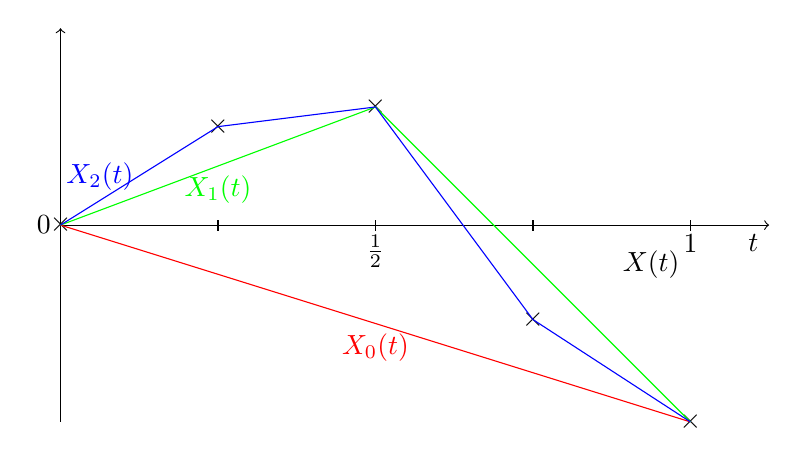
\begin{tikzpicture}
\draw[->] (0,-2.5) -- (0,2.5);
\draw[->] (0,0) -- (9,0);
\draw (0,0) node[anchor=east] {$0$};
\draw (4,0) node[anchor=north] {$\frac 12$};
\draw (8,0) node[anchor=north] {$1$};
\draw (8.8,0) node[anchor=north] {$t$};
\foreach \x in {0,2,4,6,8}
	\draw (\x cm,-2pt) -- (\x cm, 2pt);
\path (0,0) node {$\times$}--  (2,1.25)node {$\times$} -- (4,1.5) node {$\times$}--  (6,-1.2)node {$\times$} -- (8,-2.5)node {$\times$};
\draw[color=black] plot file {BBplot.data};
\draw[color=red] (0,0)  -- node[below] {$X_0(t)$} (8,-2.5);
\draw[color=green] (0,0) -- node[below] {$X_1(t)$} (4,1.5) -- (8,-2.5);
\draw[color=blue] (0,0) -- node[above,near start] {$X_2(t)$} (2,1.25) -- (4,1.5) --  (6,-1.2) -- (8,-2.5);
\draw[color=black] (7.5,-0.5) node {$X(t)$};
\end{tikzpicture}
\end{center}

\begin{beweis}

Es sei $L^2=L^2([0,1],\borel_{[0,1]}, \lambda_{[0,1]}) \da \{f :[0,1]\to \MdR\mid f \text{ messbar, } \int_0^1 f^2(x)dx <\infty\}$ beziehungsweise deren Äquivalenzklassen. Versehen mit
\[
\langle f,g \rangle \da \int_0^1 f(x)\cdot g(x) dx
\]
ist $L^2$ ein Hilbertraum. Weiter sei für alle $n\in \mathbb N_0$
\[
S_n\da\{(n,k) \mid 1\le k \le 2^n, k\text{ ungerade}\}
\]
und $S\da\bigcup_{n=0}^\infty S_n$. Definiere für $(n,k)\in S$
\begin{align*}
g_{01}(t) &\da 1\\
g_{nk}(t) &\da 2^{\frac{(n-1)}2}\big( 1_{[(k-1)2^{-n},\,k2^{-n})}(t) - 1_{[k2^{-n},\,(k+1)2^{-n})}(t)\big) \quad \text{für } n\ne 0,\,0\le t\le 1.
\end{align*}
Diese Funktionen bilden eine Orthonormalbasis (die \emph{Haar-Basis}\index{Haar-Basis}) von $L^2$, das heißt $\|g_{nk}\|=1$, $\langle g_{nk},g_{ml} \rangle = 0$ für $(n,k)\ne (m,l)$ und es gilt die sogenannte Parsevalsche Gleichung:
\[
\langle f,g\rangle = \sum_{n=0}^\infty \sum_{(n,k)\in S_n} \langle f,g_{nk}\rangle\langle g,g_{nk}\rangle
\]

Es sei nun $\{Z_{nk} \mid (n,k)\in S\}$ eine Familie von unabhängigen $\mathcal N(0,1)$-verteilten Zufallsvariablen auf einem Wahrscheinlichkeitsraum $(\Omega, \cF, P)$.

Wir definieren $(X_n(t))_{0\le t\le 1}$, $n\in \MdN_0$, durch
\begin{align*}
X_n(t) \da \sum_{m=0}^n \sum_{(m,k)\in S_m} f_{mk}(t) \cdot Z_{mk}
\end{align*}
wobei für alle $t\in[0,1], (m,k)\in S$
\begin{align*}
f_{mk}(t) \da \int_0^t g_{mk}(s) ds 
\end{align*}
die sogenannte \emph{Schauder-Funktionen} sind. Diese $(X_n(t))_{0\le t\le 1}$ sind stetige stochastische Prozesse auf $(\Omega,\cF, P)$.

Es gilt $0\le f_{nk} \le 2^{-\frac{(n+1)}2}$. Wir behaupten, dass für $P$-fast-alle $\omega\in \Omega$ die $(X_n(t,\omega))_{0\le t\le 1}$ für $n\to\infty$ gleichmäßig konvergiert. Dann wäre die Grenzfunktion $X$ automatisch stetig.

Für $Z\sim \mathcal N(0,1)$ verwenden wir ohne Beweis die Abschätzung
\[
P(|Z|\ge a) \le \sqrt {\frac2\pi}\frac 1a e^{-\frac{a^2}2}\text{ für alle }a>0.
\]

Sei $\|f\|_{\infty}\da \sup_{0\le t\le 1}|f(t)|$ für $f\in C[0,1]$. Dann gilt für alle $n\in \MdN$: 
\begin{align*}
P(\|X_n - X_{n-1}\|_{\infty} > a_n) &= P(\|\sum_{(n,k)\in S_n}f_{nk}(t) Z_{nk}\|_{\infty} > a_n) \\
&= P(\sup_{(n,k)\in S_n} |Z_{nk}| > 2^{\frac{(n+1)}2} a_n) \\
&\le \sum_{(n,k)\in S_n} P(|Z_{nk}| > 2^{\frac{(n+1)}2} a_n) \\
&= |S_n| \cdot P(|Z_{01}| > 2^{\frac{(n+1)}2} a_n) \\
&\le 2^n\cdot P(|Z_{01}| > 2^{\frac{(n+1)}2} a_n) \\
&\le 2^n\cdot \sqrt {\frac2\pi}\frac 1 {a_n} 2^{-\frac{(n+1)}2}  e^{-\frac1 2  2^{(n+1)} a_n^2} \\
\intertext{mit $a_n\da \sqrt{n2^{-n}}$ wird daraus}
&= \sqrt {\frac2\pi} 2^n 2^{-\frac{n+1}2} n^{-\frac 12} 2^{\frac n2} e^{-\frac 12 2^{n+1} n 2^{-n} } \\
&= \frac1{\sqrt \pi} 2^n n^{-\frac12} e^{-n} \\
\end{align*}
das heißt dass mit $A_n\da \{\|X_n-X_{n-1}\|_{\infty}> (n2^{-n})^{\frac12}\}$ gilt 
\begin{align*}
\sum_{n=1}^\infty P(A_n) <\infty.
\end{align*}
Nach dem Lemma von Borel-Cantelli gilt dann
\begin{align*}
P(\underbrace{\limsup_{n\to\infty} A_n}_{\ad N}) = 0.
\end{align*}
Das heißt dass für jedes $\omega \notin N$ gibt es einen Index $n_0=n_0(\omega)\in \MdN$, so dass für alle $m,n\ge n_0$ gilt:
\begin{align*}
\|X_m(\omega)-X_n(\omega)\|_\infty &\le \sum_{k=(m\wedge n)+1}^{m\vee n} \|X_k(\omega)-X_{k-1}(\omega)\|_\infty \\
&\le \sum_{k=(m\wedge n)+1}^{\infty} \sqrt{k2^{-k}} \to 0 \text{ für } m,n\to\infty
\end{align*}
Es ist also $(X_n(\omega))_{n\in \MdN}$ ist eine Cauchy-Folge in $(C[0,1],\|\cdot\|_\infty)$ für $\omega \notin N$. Dieser Raum ist vollständig, also existiert eine Grenzfunktion $X(\omega)$, wobei wir $X(\omega)\da0$ für $\omega\in N$ setzen.

Der Prozess $(X_t)_{0\le t\le 1}$ hat $P$-fast-sicher stetige Pfade. Wir zeigen nun, dass dieser Prozess ein Gauss-Prozess wie in Satz \ref{satz:9.2} ist:

Es gilt jetzt für alle $n\in\MdN$, $0\le s,t\le 1$
\begin{align*}
EX_n(t) &= \sum_{m=0}^n \sum_{(m,k)\in S_m} f_{nk}(t) \cdot EZ_{mk} \\
&= \sum_{m=0}^n \sum_{(m,k)\in S_m} f_{nk}(t) \cdot 0 \\
&= 0
\end{align*}
und, wobei die gemischten Terme verschwinden, da die $Z_{nk}$ unabhängig sind,
\begin{align*}
EX_n(t)X_n(s) &= \sum_{m=0}^n \sum_{(m,k)\in S_m} f_{nk}(t)f_{nk}(s) E{Z_{mk}}^2 \\
 &= \sum_{m=0}^n \sum_{(m,k)\in S_m} f_{nk}(t)f_{nk}(s)  \\
\intertext{Offenbar ist $f_{nk}(s)=\langle 1_{[0,s]},g_{nk}\rangle$ und mit der Parsevalschen Gleichung folgt:}
\mathllap{(*) \quad} \lim_{n\to\infty} EX_n(t)X_n(s) &= \sum_{m=0}^\infty \sum_{(m,k)\in S_m} \langle 1_{[0,s]},g_{nk}\rangle \langle 1_{[0,t]},g_{nk}\rangle \\
&= \langle 1_{[0,s]}, 1_{[0,t]}\rangle\\
&= s\wedge t
\end{align*}

Sei $t_1,\ldots,t_k\in [0,1]$. Es gilt
\[
(X_n(t_1),\ldots,X_n(t_k)) \to (X(t_1),\ldots,X(t_k))\quad \text{$P$-f.s.}
\]
woraus die Konvergenz in Verteilung folgt und, dazu äquivalent, die Konvergenz der charakteristischen Funktionen $\varphi_n:\MdR^k\to \MdC$, $\varphi_n(\theta)=E\exp(i\sum_{\nu=1}^k \theta_\nu X_n(t_\nu))$, also 
\[
\varphi_n(\theta)\tomit{n\to\infty} \varphi(\theta) = \exp(i\sum_{\nu=1}^k\theta_\nu X(t_\nu)).
\]
Es gilt $\varphi_n(\theta) = \exp(-\frac 12 \theta^\top\Sigma_n\theta)$ mit $(\Sigma_n)_{i,j}=EX_n(t_i)X_n(t_j)$. Mit $(*)$ folgt dann
\begin{align*}
\lim_{n\to\infty} (\Sigma_n)_{i,j} = t_i\wedge t_j \ad (\Sigma)_{i,j}
\intertext{also}
\varphi_n(\theta) \to \varphi(\theta) = \exp(-\frac12 \theta^\top \Sigma \theta)
\end{align*}
Daraus folgt, dass $(X_{t_1},\ldots,X_{t_k})$ normalverteilt ist, mit $EX_t=0$ für alle $t\in[0,1]$ und $\operatorname{Cov}(X_s,X_t)=s\wedge t$ für alle $s,t\in[0,1]$. Mit Satz \ref{satz:9.2} folgt die Behauptung.
\end{beweis}

\begin{bemerkung}
Auf $(C[0,1],\borel(C[0,1]))$ definiert die Verteilung $P^B$ von $(B_t)_{0\le t\le 1}$ ein Wahrscheinlichkeitsmaß, das sogenannte Wiener-Maß\index{Wiener-Maß}. Mit $(\Omega,\cF, P)=(C[0,1],\borel(C[0,1]),P^B)$ und $B_t=\pi_t$ hat man ein explizites Modell für $(B_t)_{0\le t\le 1}$, die sogenannte Kanonische Konstruktion.
\end{bemerkung}

\section{Pfadeigenschaften}

\begin{satz}
\label{satz:11.1}
Ist $(B_t)_{t\ge 0}$ eine Brownsche Bewegung auf einem Wahrscheinlichkeitsraum $(\Omega, \cF, P)$, so gilt für $P$-fast-alle $\omega\in \Omega$, dass 
\begin{align*}
\sup_{t\ge 0} B_t(\omega) = \infty, &&\inf_{t\ge 0}B_t(\omega)=-\infty.
\end{align*}
\end{satz}
\begin{beweis}
Sei $Z\da \sup_{t\ge 0}B_t$. Nach Satz \ref{satz:9.3} c) gilt für alle $c>0$:
$Z\gleichnach{d} c\cdot Z$. Da $Z\ge 0$ folgt $P(Z \in \{0,\infty\})=1$.

Nach Satz \ref{satz:9.3} b) ist $(B_{1+t}-B_1)_{t\ge 0}$ wieder eine Brownsche Bewegung, das Supremum davon ist also wieder $P$-f.s. $0$ oder $\infty$.
\begin{align*}
P(Z=0) &\le P(B_1\le 0\text{ und }B_t\le 0\text{ für alle } t\ge 1) \\
&=P(B_1\le 0 \text{ und } \sup_{t\ge 0}(B_{1+t}-B_1) \le |B_1|) \\
&= P(B_1 \le 0 \text{ und } \sup_{t\ge 0}(B_{1+t}-B_1) = 0) \\
\intertext{$(B_{1+t}-B_1)$ ist unabhängig von $B_1$, also gilt weiter}
&= P(B_1\le 0)\cdot P(\sup_{t\ge 0}(B_{1+t}-B_1) = 0) \\
&= \frac12 \cdot P(Z=0)
\end{align*}
Das heißt, dass $P(Z=0)\le \frac 12 P(Z=0)$, also muss $P(Z=0)=0$ und $P(\sup_{t\ge 0}B_t =\infty) = 1$ gelten.

Die Aussage für das Infimum folgt dann aus Satz \ref{satz:9.3} a).
\end{beweis}


\begin{bemerkung}
Für alle $a\in \MdR$ ist $\{t\ge 0\mid B_t=a\}$ $P$-fast-sicher unbeschränkt, da stetige Funktionen auf kompakten Intervallen beschränkt sind. Insbesondere kehrt $(B_t)_{t\ge 0}$ mit Wahrscheinlichkeit 1 unendlich oft nach 0 zurück, und es gibt für $P$-fast-alle $\omega\in\Omega$ eine Folge $(t_n)_{n\in \MdN}  = (t_n(\omega))_{n\in\MdN}$ mit $t_n\to \infty$ und $B_{t_n}(\omega)=0$ für alle $n\in\MdN$. Mit der Zeitumkehr $\tilde B_t=tB_{\frac 1t}$, $\tilde B_0=0$ folgt, dass für $P$-fast alle $\omega\in \Omega$ die Nullstellen des Pfades $t\to B_t(\omega)$ einen Häufungspunkt in $0$ haben.
\end{bemerkung}

\begin{definition}
Eine Funktion $f:\MdR_{+}\to \MdR$ heißt Lipschitz-stetig in $x\in\MdR_+$ wenn es ein $\delta>0$ und ein $K<\infty$ gibt mit
\[ |f(x)-f(y)| \le K|x-y|\]
für alle $y\in[x-\delta,x+\delta]\cap\MdR_+$.
\end{definition}

\begin{satz}
\label{satz:11.2}
$P$-fast-alle Pfade einer Brownschen Bewegung sind in keinem Punkt Lipschitz-stetig.
\end{satz}
\begin{beweis}
Es seien $0<a<b<\infty$ fest und $K>0$. Für $n\in\MdN$ mit $a-\frac 2n>0$ sei 
\[
A_n \da \{\omega\in \Omega\mid \exists s\in (a,b)\ \forall t\in[s-\frac2n,s+\frac2n]: |B_t(\omega) - B_s(\omega)| \le K|t-s|\}
\]
Für jedes $I=[s-\frac2n,s+\frac2n]$ gibt es ein $k\in\MdN$ mit $\frac{k-2}n,\frac{k-1}n,\frac kn,\frac{k+1}n\in I$. Auf $A_n$ gilt für $j=k-1,k,k+1$
\begin{align*}
\underbrace{|B(\frac jn)-B(\frac {j-1}n)|}_{\ad \Delta_{n,j}} &\le | B(\frac jn) - B(s)| + |B(s) - B(\frac {j-1}n)| \\
&\le K\cdot \frac 2n + K\cdot \frac 2n\\
&= \frac{4K}n
\end{align*}
Also ist 
\[
A_n\subseteq \bigcup_{k=\lfloor na\rfloor}^{\lceil nb+1\rceil} \{\omega\in \Omega\mid \Delta_{n,j}(\omega) \le \frac{4K}n\text{ für }j=k-1,k,k+1\}
\]
Die Zuwächse der Brownschen Bewegung sind unabhängig, also folgt:
\begin{align*}
P(A_n) &\le \sum_{k=\lfloor na\rfloor}^{\lceil nb+1\rceil} P\Big(\Delta_{n,k-1}\le \frac{4K}n\Big)\cdot P\Big(\Delta_{n,k}\le \frac{4K}n\Big)\cdot P\Big(\Delta_{n,k+1}\le \frac{4K}n\Big) \\
&\le {\lceil nb+1\rceil}\cdot P\Big(\Delta_{n,1}\le \frac{4K}n\Big)^3
\end{align*}
Da $\sqrt{n}(B(\frac{1}{n})-B(\frac{0}{n}))\sim\mathcal N(0,1)$ folgt
\begin{align*}
  P\Big(\Delta_{n,1}\leq\frac{4k}{n}\Big) &=P\Big(\Delta_{n,1}\sqrt{n}\leq\frac{4k}{\sqrt{n}}\Big) \\
  &=\int_{-\frac{4k}{\sqrt{n}}}^{\frac{4k}{\sqrt{n}}}\frac{1}{\sqrt{2\pi}}e^{\frac{x^2}{2}}dx\leq\frac{8k}{\sqrt{2\pi n}} \\
\end{align*}
und insgesamt $P(A_n)\longrightarrow 0$ für $n\longrightarrow\infty$. \\
Sei $n_0(a):=\inf\left\{n\in\mathbb N\mid a-\frac{2}{n} > 0\right\}$. Wegen $A_n\subset A_{n+1}$
folgt für $A:=\bigcup_{n=n_0}^\infty A_n$, dass $P(A)=0$. \\
$A=A(k)$ hängt von $k$ ab. $N:=\bigcup_{k\in\mathbb N}A(k)$ ist wieder eine Nullmenge, so dass
$\forall \omega\notin N$ gilt: zu keinem $s\in(a,b)$ und keinem $\delta > 0$, $\exists k<\infty$ mit
\[
\vert B_t(\omega)-B_s(\omega)\vert\leq k\vert t-s\vert\text{ mit }t\in[s-\delta,s+\delta]
\]
$\implies$ Die Pfade, die in einem $s\in (a,b)$ lipschitzstetig sind, sind in einer $P$-Nullmenge. \\
 \[ 
N=\mathcal N(a,b)\implies\tilde{N}=\bigcup_{\begin{array}{c} k\in\mathbb N \\ a=\frac{1}{k},b=k \end{array}} \mathcal N(a,b)\text{ ist wieder Nullmenge }
\]
$\implies$ $P$-f.a. Pfade sind in keinem $s>0$ lipschitzstetig. Bleibt $s=0$ (Übung)  

\end{beweis}

\begin{bemerkung}
  Ist eine Funktion $f:\mathbb R_+\longrightarrow\mathbb R$ in $s\in \mathbb R$ differenzierbar, so existiert
\[
\lim_{t\rightarrow s}\frac{f(t)-f(s)}{t-s}
\]
und $f$ wäre in $s$ lipschitzstetig. Satz 11.2 impliziert also, dass $P$-f.a. Pfade der Brownschen Bewegung in keinem Punkt differenzierbar sind.
\end{bemerkung}

\begin{definition}
  Sei $f:\mathbb R_+\longrightarrow\mathbb R$. Die Totalvariation $V_a^b f$ von $f$ auf $[a,b]\subset\mathbb R_+$ ist
\[
V_a^bf=\sup_{\mathcal Z}\sum_{j=1}^n\vert f(t_j)-f(t_{j-1})\vert,
\]
wobei $\mathcal Z=\{a=t_0<t_1<\dots<t_n=b\}$ eine Zerlegung von $[a,b]$ ist.
\end{definition}

\begin{bemerkung}
  Funktionen mit endlicher Totalvariation sind fast überall differenzierbar. Also haben die Pfade der Brownschen Bewegung $P$-f.s. unbeschränkte Totalvariation, d.h. auch kleine Stücke sind ``unendlich lang''.
\end{bemerkung}

\begin{definition}
  Sind die ZV $X,X_1,X_2,\dots\in L^2(\Omega,\cF,P)$, so heißt die Folge $(X_n)_{n\in\mathbb N}$ im \emph{quadratischen Mittel konvergent} gegen $X$ ($X_n\tomit{L^2} X$), falls gilt:
\[
\lim_{n\rightarrow\infty}E(X_n-X)^2=0
\]
\end{definition}
\begin{bemerkung}
  $X_n\tomit{L^2}X\implies X_n\tomit{P}X$.
\end{bemerkung}
\begin{satz}
  \label{Satz 11.3}
  Es sei $(\mathcal Z_n), \mathcal Z_n=\{0=t_{n_0}\leq t_{n_1}\leq\dots\leq t_{n_{k_n}}=t\}$ eine Folge von Zerlegungen von $[0,t]$ mit Feinheitsgraden
\[
\delta(\mathcal Z_n)=\max_{j=1,\dots,k_n}\vert t_{n_j}-t_{n_{j-1}}\vert
\]
so dass $\lim_{n\rightarrow\infty}\delta(\mathcal Z_n)=0$. Dann gilt mit $n\to\infty$:
\[
\underbrace{\sum_{j=1}^{k_n}(B(t_{n_j})-B(t_{n_{j-1}}))^2}_{=:V_{\mathcal Z_n}}\tomit{L^2}t
\] 
\end{satz}
\begin{beweis}
  Zu zeigen ist: $E(V_{\mathcal Z_n}-t)^2\to 0$ für $n\to\infty$. Es gilt:
  \begin{enumerate}
  \item $EV_{\mathcal Z_n}=\sum_{j=1}^{k_n}(t_{n_j}-t_{n_{j-1}})=t$
  \item $E(B(t_{n_j})-B(t_{n_{j-1}}))^4=3(t_{n_j}-t_{n_{j-1}})^2$
  \end{enumerate}
Insgesamt:
\begin{align*}
  EV_{\mathcal Z_n}^2 &= \sum_{j=1}^{k_n}E(B(t_{n_j})-B(t_{n_{j-1}}))^4+2\sum_{j<l}E(B(t_{n_j})-B(t_{n_{j-1}}))^2\cdot E(B(t_{n_j})-B(t_{n_{j-1}}))^2 \\
&=3\left(\sum_{j=1}^{k_n}(t_{n_j}-t_{n_{j-1}})\right)^2+2\sum_{j=1}^{k_n}(t_{n_j}-t_{n_{j-1}})^2 \\
&=t^2+2\sum_{j=1}^{k_n}(t_{n_j}-t_{n_{j-1}})^2
\end{align*}
\begin{align*}
  \implies E(V_{\mathcal Z_n}-t)^2 &= EV_{\mathcal Z_n}^2-2t^2+t^2 \\
&= 2\sum_{j=1}^{k_n}(t_{n_j}-t_{n_{j-1}})^2 \\
& \leq 2\delta(\mathcal Z_n)\cdot t\to 0 \text{ für } n\to\infty
\end{align*}
\end{beweis}
\begin{bemerkung}
  Beachte, dass die Zerlegungsfolge $\mathcal Z_n$ nicht von $\omega$ abhängt. Gilt zusätzlich $\mathcal Z_n\subset\mathcal Z_{n+1}$, so gilt sogar $V_{\mathcal Z_n}\tomit{f.s.}t$. Dieser Grenzwert heißt quadratische Variation des Prozesses.
\end{bemerkung}
\begin{bemerkung}
  Eine stetige Funktion $f$ auf einem kompakten Intervall $[a,b]$ mit $V_a^bf<\infty$, hat stets quadratische Variation $0$, da
  \[
    \sum_{k=1}^n(f(t_k)-f(t_{k-1}))^2 \leq\max_{1\leq k\leq n}\vert f(t_k)-f(t_{k-1})\vert\cdot\sum_{i=1}^n\vert f(t_k)-f(t_{k-1})\vert
  \]
Also $V_a^b B(\cdot,\omega)=\infty\quad\forall 0\leq a<b<\infty$.
\end{bemerkung}
\section{Die Brownsche Bewegung als Markov-Prozess}
\begin{definition}
  Ein \emph{stochastischer Kern}\index{stochastischer Kern} (Übergangswahrscheinlichkeit) $P(x,A)$ von $(\mathbb R, \borel)$ nach $(\mathbb R, \borel)$ ist eine Funktion, so dass
  \begin{enuma}
  \item für alle $x\in \MdR$ ist $A\mapsto P(x,A)$ ein Wahrscheinlichkeitsmaß und
  \item für alle $A\in\borel$ ist  $x\mapsto P(x,A)$ messbar.
  \end{enuma}
\end{definition}
\begin{definition}
    Eine Familie $(P_t)_{t\geq 0}$ von stochastischen Kernen von $(\mathbb R, \borel)$ nach $(\mathbb R, \borel)$ heißt \emph{Markov-Halbgruppe}\index{Markov-Halbgruppe} oder \emph{Übergangs-Halbgruppe}\index{Übergangs-Halbgruppe}, wenn für alle $s,t\ge 0$ und für alle $A\in\borel$ gilt:
\[
P_{s+t}(x,A)=\int P_t(y,A)P_s(x,dy)
\]
\end{definition}
\begin{bemerkung}
  Wir schreiben kurz: $P_{s+t}=P_s\otimes P_t$.
\end{bemerkung}
\begin{beispiel}
Für $t\ge 0$ sei $P_t(x,\cdot)=\mathcal N(x,t)$ die Normalverteilung mit Erwartungswert $x$ und Varianz $t$, wobei $\mathcal N(x,0):=\delta_x$.
\[
P_t(x,A) = \int_A \frac1{\sqrt{2\pi t}} e^{-\frac 1{2t}(y-x)^2}dy
\]
ist messbar (Fubini) und es gilt
\begin{align*}
\int P_t(y,A)P_s(x,dy) &= \int_A \Big(\int \underbrace{\frac1{\sqrt{2\pi t}}e^{-\frac1{2t}(z-y)^2}}_{\ad f_2(z-y)} \underbrace{\frac1{\sqrt{2\pi s}} e^{-\frac1{2s} (y-x)^2}}_{\ad f_1(y)} dy \Big) dz \\
&= \int_A\Big(\int f_2(z-y)\cdot f_1(y) dy\Big) dz \\
%&= \mathcal N(0,t)*\mathcal N(x,s) \\
%&= \mathcal N(x,s+t) \\
&= P_{s+t}(x,A).
\end{align*}
\end{beispiel}

\begin{definition}
Es seien $(\Omega, \cF, P)$ ein Wahrscheinlichkeitsraum mit Filtration $(\cF_t)_{t\ge 0}$, $(X_t)_{t\ge 0}$ ein dazu adaptierter reellwertiger Prozess, $\nu$ ein Wahrscheinlichkeitsmaß auf $(\MdR, \borel)$ und $(P_t)_{t\ge 0}$ eine Markov-Halbgruppe. Gilt dann $X_0\sim \nu$ und für alle $0\le s\le t$, $A\in\borel$
\begin{align*}
P(X_t\in A\mid \cF_s) = P_{t-s}(X_s,A)\tag{$*$}
\end{align*}
so heißt $(X_t,\cF_t)_{t\ge 0}$ ein (homogener) \emph{Markov-Prozess}\label{Markov-Prozess!allgemeiner} mit Übergangshalbgruppe $(P_t)_{t\ge 0}$ und Startverteilung $\nu$.
\end{definition}

\begin{bemerkung}
\begin{enuma}
\item In der Regel ist $(\cF_t)_{t\ge 0}$ die natürliche Filtration zu $(X_t)_{t\ge 0}$.
\item Zum Nachweis von $(*)$ genügt zu zeigen, dass für alle $F\in \cF_s$, $A\in \borel$
\begin{align*}
\underbrace{\int_F 1_{[X_t\in A]} dP}_{P(F\cap \{X_t\in A\})} = \int_F(P_{t-s})(X_s,A)dP
\end{align*}
da $P_{t-s}(X_s,A)$ als messbare Funktion von $X_s$ $\cF_s$-messbar ist.

Besitzt $\cF_s$ einen durchschnittsstabilen Erzeuger $\mathcal E$, so genügt es, die Gleichung für alle $F\in\mathcal E$ nachzuprüfen.
\end{enuma}
\end{bemerkung}

\begin{satz}
\label{satz:12.1}Es sei $(B_t)_{t\ge 0}$ die Brownsche Bewegung mit zugehöriger natürlicher Filtration $(\cF_t)_{t\ge 0}$. Dann ist $(B_t,\cF_t)_{t\ge 0}$ ein Markov-Prozess mit Startverteilung $\delta_0$ und stochastischen Kernen $P_t(x,\cdot)=\mathcal N(x,t)$.
\end{satz}

\begin{beweis}
Wir zeigen zunächst eine Hilfsaussage: Seien $0=t_0\le t_1\le \cdots \le t_n$ und $g:\MdR^n\to \MdR$ eine beschränkte $(\borel^n,\borel)$-messbare Funktion. Setze $Y_i=B_{t_i}-B_{t_{i-1}}$ für $i=1,\ldots,n$. $Y_1,\ldots,Y_n$ sind unabhängig und $Y_i\sim\mathcal N(0,t_i-t_{i-1})$. Also gilt:
\begin{align*}
Eg(B_{t_1},\ldots,B_{t_n}) &= Eg(Y_1,Y_1+Y_2,\ldots,Y_1+\cdots +Y_n) \tag{$\triangle$}\\
&= 
\int\cdots\int g(y_1,y_1+y_2,\ldots,y_1+\cdots +y_n) \\
&\quad\quad 
\mathcal N(0,t_n-t_{n-1})(dy_n) \mathcal N(0,t_{n-1}-t_{n-2})(dy_{n-1})\cdot \mathcal N(0,t_1)(dy_1)\\
&= \int\cdots\int g(x_1),\ldots,g(x_n) \mathcal N(x_{n-1},t_n-t_{n-1})(dx_n) \cdots \mathcal N(0,t_1)(dx_1)
\end{align*}
Es sei $A\in \borel$, $0\le s\le t$. Zu zeigen ist, dass $P(B_t\in A\mid \cF_s) = \mathcal N(B_s,t-s)(A)$, das heißt
\begin{align*}
\int_F 1_{[B_t\in A]} dP = \int_F\mathcal N(B_s,t-s)(A)dP \tag{$\square$}
\end{align*}
für alle $F\in \cF_s$, beziehungsweise auf einem durchschnittsstabilen Erzeugendensystem von $\cF_s$. Ein solcher ist
\begin{align*}
\bigcap_{k=1}^n \{B_{t_k}\in A_k\}\quad 0\le t_1\le \cdots\le t_n=s,\, A_1\ldots,A_n\in \borel.
\end{align*}
Setze $g(x_1,\ldots,x_n,x)= 1_A(x)\cdot \prod_{k=1}^n(1_{A_k}(x_k))$ in $(\triangle)$:
\begin{align*}
Eg(B_{t_1},\ldots,B_{t_n}) &= Eg(Y_1,Y_1+Y_2,\ldots,Y_1+Y_n) \\
&=\int_{A_1}\cdots\int_{A_n}\int_A \mathcal N(x_n,t-s)(dx)\mathcal N(x_{n-1},t_n-t_{n-1})(dx_n)\cdots N(0,t_1)(dx_1) \\
&= \text{linke Seite von ($\square$) mit obigen $F$}
\end{align*}
Setze jetzt $g(x_1,\ldots,x_n) = \mathcal N(x_n,t-s)(A)\prod_{k=1}^n 1_{A_k}(x_k)$ in $(\triangle)$:
\begin{align*}
Eg(B_{t_1},\ldots,B_{t_n}) &= \int\cdots\int_{\{B(t_1)\in A_1,\ldots,B(t_n)\in A_n\}} \mathcal N(x_n,t-s)(A) dP\\
&= \int_{A_1}\cdots\int_{A_n} \mathcal N (x_n,t-s)(A) N(x_{n-1},t_n-t_{n-1})(dx_n) \cdots \mathcal N(0,t_1)(dx_1)\\
&= \text{rechte Seite von ($\square$) mit obigen $F$}
\end{align*}
Da $\int_A\mathcal N(x_n,t-s)(dx) = \mathcal N(x_n,t-s)(A)$ ist $(\square)$ gezeigt.
\end{beweis}

\begin{bemerkung}
Die Markov-Eigenschaft lässt sich schreiben als
\begin{align*}
P(X_{s+t}\in A\mid \cF_s) = P_t(X_s,A) \tag{$*$}
\end{align*}
für alle $A\in\borel$, $s,t\ge 0$.

Definiere für $f:\MdR\to\MdR$ (oder $\to \MdC$), falls existent, für alle $x\in \MdR$:
\begin{align*}
\big(P_tf\big)(x) \da \int f(y) P_t(x,dy)
\end{align*}
Also kann man schreiben:
\begin{align*}
P_t(X_s,A) = \int 1_A(y) P_t(X_s,dy) = \big(P_t1_A\big)(X_s)
\end{align*}
für $f=1_A$ kann man $(*)$ schreiben als
\begin{align*}
E[f(X_{s+t}) \mid \cF_s] = \big(P_tf\big) (X_s) \tag{$\triangle$}
\end{align*}
Mittels Algebraischer Induktion und der monotonen Konvergenz in bedingter Version kann man daraus folgern, dass die Gleichung ($\triangle$) für alle messbaren, beschränkten $f:\MdR\to\MdR$ gilt.

Umgekehrt stellt sich die Frage: Für welche Funktionenklasse muss die Gleichung $(\triangle)$ gelten, um $(*)$ zu folgern?

Für $s=0$ und $\cF_s=\{\emptyset, \Omega\}$ folgt $(*)$, wenn $(\triangle)$ für alle $f:\MdR\to \MdC$ der Form $f(x) = e^{i\theta x}$, $\theta\in \MdR$ gilt. (Eindeutigkeitssatz für charakteristische Funktionen)

Dies gilt auch für bedingte charakteristische Funktionen, das heißt $(*)$ ist erfüllt, wenn für alle $\theta\in \MdR$ gilt:
\begin{align*}
E[e^{i\theta X_{s+t}}\mid \cF_s] = \int e^{i\theta y}P_t(X_s,dy).
\end{align*}

Damit kann man Satz \ref{satz:12.1} direkt zeigen:
\begin{align*}
E[e^{i\theta B_{s+t}}\mid \cF_s] &= E[e^{i\theta(B_s+B_{s+t}-B_s)}\mid \cF] \\
&= e^{i\theta B_s} \cdot E[e^{i\theta B_{s+t}-B_s}] \\
&= e^{i\theta B_s} \cdot e^{-\theta^2\frac t2} \\
&= \int e^{i\theta y}P_t(B_s,dy)
\end{align*}
\end{bemerkung}

In Kapitel II haben wir gesehen, dass die Übergangsmatrizenfunktion $(P(t))_{t\geq0}$ durch die Intensitätsmatrix $Q$ in bestimmten Fällen charakterisiert werden kann. \\
Insbesondere ist:
\[
q_{ij}:=\lim_{t\downarrow0}\frac{p_{ij}(t)-\delta_{ij}}{t}
\]
Unter bestimmten Voraussetzungen kann auch $(P_t)_{t\geq0}$ bei allgemeinen Markov-Prozessen aus dem sogenannten Generator
\[
\mathcal G:=\lim_{t\downarrow0}\frac{1}{t}(P_t-P_0)
\]
bestimmt werden. Wir betrachten hier die Brownsche Bewegung.
\[
C_b^2(\mathbb R):=\{f:\mathbb R\to\mathbb R\mid f \text{ ist zweimal stetig differenzierbar, $f$ beschränkt}\}
\]
\begin{satz}
\label{satz:12.2}
  Es sei $(P_t)_{t\geq0}$ die Übergangshalbgruppe zur Brownschen Bewegung. Dann gilt:
\[
\mathcal Gf:=\lim_{t\downarrow0}\frac{1}{t}(P_tf-f)=\frac{1}{2}f''\text{ für alle }f\in C_b^2(\mathbb R)
\]
\end{satz}
\begin{beweis}
  Sei $f\in C_b^2(\mathbb R)$.
  \begin{align*}
    \frac{1}{t}(P_tf-f)(x)&=\int\frac{1}{t}(f(y)-f(x))\mathcal N(x,t)(dy) \\
&=\frac{1}{\sqrt{2\pi}}\int t^{-\frac{3}{2}}(f(y)-f(x))e^{-\frac{(y-x)^2}{2t}}dy =(*)
  \end{align*}
Substitution mit $z=\frac{y-x}{\sqrt{t}}$ liefert:
\[
(*)=\frac{1}{\sqrt{2\pi}}\int\frac{1}{t}(f(x+z\sqrt{t})-f(x))e^{-\frac{1}{2}z^2}dz
\]
Taylor-Entwicklung:
\[
f(x+z\sqrt{t})=f(x)+z\sqrt{t}f'(x)+\frac{1}{2} z^2tf''(\xi)\text{ mit }\xi\in(x,x+z\sqrt{t})
\]
Daraus folgt:
\[
\frac{1}{t}(P_tf-f)(x)=\frac{1}{\sqrt{2\pi}}\frac{f'(x)}{\sqrt{t}}\int ze^{-\frac{1}{2}z^2}dz+\frac{1}{2}\int\frac{1}{\sqrt{2\pi}}z^2f''(\xi)e^{-\frac{1}{2}z^2}dz
\]
Es gilt: $f''(\xi)\to f''(x)$ für $t\to0$. Da $f''$ beschränkt ist, folgt mit majorisierter Konvergenz:
\[
\lim_{t\downarrow0}\frac{1}{t}(P_tf-f)(x)=\frac{1}{2}f''(x)\underbrace{\int\frac{1}{\sqrt{2\pi}}z^2e^{-\frac{1}{2}z^2}dz}_{=1}
\]
\end{beweis}
\section{Die starke Markov-Eigenschaft mit Anwendungen}
Wir benötigen zunächst folgende Hilfsüberlegungen: \\
Ist $\tau:\Omega\longrightarrow[0,\infty]$ eine Stoppzeit, so ist
\[
\cF_\tau:=\{A\in\cF\mid A\cap\{\tau\leq t\}\in\cF_t\text{ für alle } t\geq0\}
\]
die $\sigma$-Algebra der $\tau$-Vergangenheit (vgl. Stochastik II).

\begin{lemma}
\label{lemma:13.1}
  \begin{enuma}
  \item Ist $\tau$ eine Stoppzeit, so wird durch
\[
\tau_n(\omega):=\left\{\begin{array}{cc}\frac{\lceil2^n\tau(\omega)\rceil}{2^n} &,\text{falls } \tau(\omega)<\infty \\ \infty &,\text{falls } \tau(\omega)=\infty\end{array}\right.
\]
eine Folge $(\tau_n)_{n\in\mathbb N}$ von Stoppzeiten definiert, die für $n\to\infty$ fast sicher gegen $\tau$ konvergiert. \\
Ist $\tau$ beschränkt, so nimmt jedes $\tau_n$ nur endlich viele Werte an.
\item Ist $X=(X_t)_{t\geq0}$ ein $(\cF_t)_{t\geq0}$ adaptierter Prozess mit rechtsseitig stetigen Pfaden, so ist für alle $t\geq0$ die Abbildung
\[
[0,t]\times\Omega\ni(s,\omega)\mapsto X_s(\omega)\in\mathbb R
\]
$\borel[0,t]\otimes\cF_t$-messbar.
\item Ist $\tau$ eine endliche Stoppzeit und $(X_t)_{t\geq0}$ ein adaptierter Prozess mit rechtsseitig stetigen Pfaden, so ist
\[
X_\tau:\Omega\longrightarrow\mathbb R, \omega\mapsto X_{\tau(\omega)}(\omega)
\]
$\cF_t$-messbar.
  \end{enuma}
\end{lemma}
\begin{bemerkung}
  Einen stochastischen Prozess $X$ mit der Messbarkeitseigenschaft aus Teil b.) nennt man \emph{progressiv messbar}.
\end{bemerkung}
\begin{beweis}
  \begin{enuma}
  \item Es ist zu zeigen, dass $\tau_n$ eine Stoppzeit ist:
\[
\{\tau_n\leq t\}=\left\{\tau\leq\underbrace{\frac{\lceil 2^nt\rceil}{2^n}}_{\leq t}\right\}\in\cF_t\text{ für alle }t\geq0.
  \]
Die anderen Aussagen sind ``klar''.
\item Wir zeigen zunächst:
\[
(s,\omega)\mapsto1_{[u,v)}(s)\cdot X_v(\omega)
\]
ist $\borel[0,t]\otimes\cF_t$-messbar für $0\leq u<v\leq t$. Denn: Sei $A\in\borel$ mit $0\notin A$, dann ist
\[
(1_{[u,v)}X_v)^{-1}(A)=\underbrace{[u,v)}_{\in\borel[0,t]}\times\underbrace{X_v^{-1}(A)}_{\cF_v\subset\cF_t}
\]
Analog: $(s,\omega)\mapsto1_{t}(s)X_t(\omega)$ ist messbar.
Sei jetzt: 
\[
X^{(n)}(s,\omega):=\sum_{k=0}^{n-1}1_{[\frac{kt}{n},\frac{(k+1)t}{n})}(s)\cdot X(\frac{(k+1)t}{n},\omega)+1_{t}(s)\cdot X_t(\omega)
\]
$X^{(n)}$ ist eine Linearkombination von Abbildungen vom obigen Typ, also $\borel[0,t]\otimes\cF_t$-messbar.
\item Es ist zu zeigen: Für alle $A\in\borel$ und $t\geq0$ ist
\[
X_t^{-1}(A)\cap\{\tau\leq t\}\in\cF_t
\]
Wir betrachten die Abbildungen:
\begin{align*}
  & g:\Omega\longrightarrow\times\Omega ,g(\omega)=(\tau(\omega)\wedge t,\omega) \\
  & h:[0,t]\times\Omega\longrightarrow\mathbb R ,h(s,\omega)=X_s(\omega)
\end{align*}
mit der $\sigma$-Algebra $\borel[0,t]\otimes\cF_t$ auf $[0,t]\times\Omega$. $g$ ist $(\cF_t,\borel[0,t]\otimes\cF_t)$-messbar, da für alle $A\in\cF_t, s\leq t$ gilt:
\[
\{\omega\in\Omega\mid(\tau(\omega)\wedge t,\omega)\in[0,s]\times A\}=A\cap\underbrace{\{\tau\leq s\}}_{\in\cF_s}\in\cF_t
\]
Die Messbarkeit von $h$ folgt aus b.). Es gilt also:
\begin{align*}
  & h(g(\omega))=h(\tau(\omega)\wedge t,\omega)=X_{\tau(\omega)\wedge t}(\omega)\text{ ist $(\cF_t,\borel)$-messbar} \\
\implies & X_{\tau\wedge t}^{-1}(A)\in\cF_t\text{ für alle }A\in\borel \\
\implies & X_\tau^{-1}(A)\cap\{\tau\leq t\}=\underbrace{X_{\tau\wedge t}^{-1}(A)}_{\in\cF_t}\cap\underbrace{\{\tau\leq t\}}_{\in\cF_t}\in\cF_t
\end{align*}
  \end{enuma}
\end{beweis}
\begin{satz}
  \label{satz:13.2}
Es sei $(B_t,\cF_t)_{t\geq0}$ eine Brownsche Bewegung, $\tau$ eine endliche Stoppzeit. Dann sind die $\sigma$"~Algebra $\cF_\tau$ und der Prozess $(B_{\tau+t}-B_{\tau})_{t\geq0}$ stochastisch unabhängig und $(B_{\tau+t}-B_{\tau})_{t\geq0}$ hat dieselbe Verteilung wie $(B_t)_{t\geq0}$.
\end{satz}

\begin{beweis}
Wir zeigen zunächst: Für alle $t\ge 0$ ist $B_{\tau+t}-B_\tau$ unabhängig von $\cF_\tau$ und hat Verteilung $\mathcal N(0,t)$. Angenommen, $\tau$ nimmt nur abzählbar viele Werte an. Dann gilt für alle $A\in \cF_\tau$, $C\in \borel$, dass
\begin{align*}
P(A\cap \{B_{\tau + t}-B_\tau \in C\}) 
&= \sum_{s\ge 0} P(\underbrace{A\cap \{\tau = s\}}_{\in \cF_s} \cap \{B_{\tau +t} - B_\tau \in C\}) \\
&= \sum_{s\ge 0} P(A\cap \{\tau =s\})\cdot\underbrace{ P(B_{s+t}-B_s\in C)}_{\mathcal N(0,t)(C)}\\
&= P(A) \cdot \mathcal N(0,t)(C).
\end{align*}
Mit $A=\Omega$ ergibt das: 
\begin{align*}
P(B_{\tau + t} - B_\tau \in C) = \mathcal N(0,t)(C)
\end{align*}
und für alle $A\in \cF_\tau $ und $C\in \borel$ gilt
\begin{align*}
P(A\cap \{B_{\tau +t} - B_\tau \in C\}) = P(A) \cdot P(B_{\tau +t}-B_\tau\in C).
\end{align*}

Sei jetzt $\tau$ eine beliebige (endliche) Stoppzeit und 
\begin{align*}
\tau_n \da \frac{ \lceil 2^n\tau \rceil}{2^n}.
\end{align*}
Wegen $\cF_\tau\subset\cF_{\tau_n}$ folgt für alle $A\in\cF_\tau$:
\begin{align*}
P(A \cap \{B_{\tau_n+t} - B_{\tau_n}\in C\})  
&= P(A) \cdot \mathcal N(0,t)(C)
\end{align*}
Für die Unabhängigkeit genügt es, $C=(-\infty, c)$, $c\in \MdR$, zu betrachten, da diese ein durchschnittsstabiles Erzeugendensystem von $\borel$ bilden.

Es bleibt zu zeigen:
\begin{align*}
\lim_{n\to\infty} \int_A 1_{(-\infty,c)} (B_{\tau_n +t}- B_{\tau_n}) dP 
&= \int_A 1_{(-\infty,c)} (B_{\tau+t}-B_\tau) dP \tag{$*$}
\end{align*}
Stetigkeit der Pfade impliziert $B_{\tau_n} \to B_\tau$, $B_{\tau_n+t}\to B_{\tau+t}$ mit $n\to \infty$ und mit majorisierter Konvergenz ($1_{(-\infty,c)} \le 1$) folgt
\begin{align*}
\lim_{n\to\infty} \int_A 1_{(-\infty,c)} (B_{\tau_n +t} - B_{\tau_n}) dP 
&= \int_A \lim_{n\to\infty} 1_{(-\infty,c)} (B_{\tau_n+t} - B_{\tau_n}) dP
\end{align*}
Das Problem ist nun, dass die Indikatorfunktion nicht stetig ist. Jedoch ist $B_{\tau _n+t}-B_{\tau _n}\sim \mathcal N(0,t)$, also ist $B_{\tau +t} - B_{\tau} \sim \mathcal N(0,t)$ und $P(B_{\tau+t}-B_\tau= c) = 0$, und damit gilt $(*)$.
Damit ist die Anfangsbehauptung gezeigt.

Sei jetzt $A\in \cF_\tau$, $0\ad t_0 < t_1 <\cdots < t_n$, $C_1,\ldots,C_n\in \borel$. Wende die bisher bewiesene Aussage auf die Stoppzeiten $\tau + t_{n-1},\tau + t_{n-2},\ldots,\tau+t_0$ an, so folgt:
\begin{align*}
P(A\cap \bigcap_{k=1}^n \{B(\tau + t_k) - B(\tau +t_{k-1}) \in C_k\}) 
&=  P(A) \cdot \prod_{k=1}^nP(B(\tau+t_k) - B(\tau + t_{k-1}) \in C_k)
\end{align*}
Da die Mengen 
\begin{align*}
\bigcup_{k=1}^n \{B(\tau +t_k) - B(\tau +t_{k-1}) \in C_k\}
\end{align*}
ein durchschnittsstabiles Erzeugendensystem der von $(B_{\tau +t}-B_\tau)_{t\ge 0}$ erzeugten $\sigma$"~Algebra bilden, folgt die Unahbhängigkeit. Analog folgt die Verteilungsaussage.
\end{beweis}

\begin{bemerkung}
$(B_{\tau \wedge t})_{t\ge 0}$ heißt Prä-$\tau$-Prozess, $(B_{\tau+t}-B_\tau)_{t\ge 0}$ heißt Post-$\tau$-Prozess.
\end{bemerkung}

\begin{satz}[Das Spiegelungsprinzip]
\label{satz:13.3}
Es sei $(B_t)_{t\ge 0}$ die Brownsche Bewegung, $\tau$ eine endliche Stoppzeit. Dann ist auch der ab $\tau$ gespiegelte Prozess $(\tilde B_t)_{t\ge 0}$:
\begin{align*}
\tilde B_t(\omega) \da 
\begin{cases}
2B_{\tau (\omega)}(\omega)-B_t(\omega),& t\ge \tau(\omega) \\
B_t(\omega), & t< \tau(\omega)
\end{cases}
\end{align*}
eine Brownsche Bewegung.
\end{satz}

% Generated by this code:
%
% from random import normalvariate
% 
% mirror = 6
% vals = []
% def intp(x, y, vx, vy):
%         m = (x+y)/2
%         vm = normalvariate(0,(x-y)/2) + (vx+vy)/2
% 
%         if (y-x) > 1.0/16:
%                 intp(x,m,vx,vm)
%         vals.append((m, vm))
%         if (y-x) > 1.0/16:
%                 intp(m,y,vm,vy)
% vals.append((0,0))
% intp(0, 8.0, 0, 2.0)
% vals.append((8.0,2.0))
% 
% f1 = open('BBplot2.data','w')
% f2 = open('BBplot2-spiegel.data','w')
% a = None
% for x, vx in vals:
% 	if a is None and x > mirror:
% 		a = vx
% 	if a is None:
% 		f1.write("%f %f\n" % (x,vx))
% 		f2.write("%f %f\n" % (x,vx))
% 	else:
% 		f1.write("%f %f\n" % (x,vx))
% 		f2.write("%f %f\n" % (x,2*a-vx))


\begin{center}
\begin{tikzpicture}
\draw[->] (0,0) -- (0,6);
\draw[->] (0,0) -- (9,0);
\draw (0,0) node[anchor=east] {$0$};
\draw (4,0) node[anchor=north] {$\frac 12$};
\draw (8,0) node[anchor=north] {$1$};
\draw (8.8,0) node[anchor=north] {$t$};
\draw (0,4.382826) node[anchor=east] {$a$};
\draw[dotted] (0,4.289879) -- (9,4.382826);
\draw (6,0) node[anchor=north] {$\tau_a$};
\draw[dotted] (6,0) -- (6,6);
\foreach \x in {0,2,4,6,8}
	\draw (\x cm,-2pt) -- (\x cm, 2pt);
\draw[color=green] plot file {BBplot2-spiegel.data};
\draw[color=black] plot file {BBplot2.data};
\draw (8,3) node {$B_t$};
\draw[color=green] (8,6) node {$\tilde B_t$};
\end{tikzpicture}
\end{center}

\begin{beweis}
Es sei $X_t \da B_{\tau\wedge t}$, $Y_t\da B_{\tau+t}-B_\tau$, $t\ge 0$. Sei jetzt 
\begin{align*}
\psi: [0,\infty) \times C[0,\infty) \times C[0,\infty) &\to C[0,\infty) \\
(a, f , g) &\mapsto h
\end{align*}
wobei
\begin{align*}
h(t) \da 
\begin{cases}
f(t), &\text{falls } t\le a \\
f(a) + g(t-a), &\text{sonst}
\end{cases}
\end{align*}
Nun ist $B= \psi(\tau, X, Y)$. Nach Satz \ref{satz:13.2} ist $(\tau,X)$ unabhängig von $Y$ und $Y$ ist eine Brownsche Bewegung, also ist $(\tau, X)$ unabhängig von $-Y$ und $-Y$ ist eine Brownsche Bewegung, das heißt
\begin{align*}
(\tau,X,Y) \gleichnach{d} (\tau,X,-Y)
\end{align*}
also ist $B=\psi(\tau,X,Y) \gleichnach{d} \psi(\tau,X,-Y)=\tilde B$.
\end{beweis}

Eine klassische Anwendung des Spiegelungsprinzip ist die Bestimmung der Verteilung von 
\[
M_t \da \sup_{0\le s\le t}B_s.
\]
Dazu betrachten wir die Stoppzeit 
\begin{align*}
\tau_a \da \inf\{t\ge 0\mid B_t=a\}
\end{align*}
für ein $a\in \MdR$ (wobei wir $\inf\emptyset = \infty$ setzen).

\begin{satz}
Es sei $t\ge 0$. Dann haben $M_t$, $M_t-B_t$ und $|B_t|$ dieselbe Verteilung.
\end{satz}

\begin{beweis}
Es sie $x>0$ und $y<x$. Sei $f:[0,t]\to \MdR$ so, dass $f(0)=0$, $f(t)\le y$, $\max_{0\le s\le t}f(s) \ge x$. Es sei 
\begin{align*}
g(s) = 
\begin{cases}
f(s), &s\le \tau_x\\
2x-f(s), &s>\tau _x
\end{cases}
\end{align*}
also ist $g(0)=0$ und $g(t) \ge 2x-y$. Dann ist 
\begin{align*}
P(M_t\ge x, B_t\le y) &= P(\tilde B_t\ge 2x-y) \\
&\gleichnach{\ref{satz:13.3}} P(B_t\ge 2x-y) \\
&=P\left(\frac{B_t}{\sqrt{t}}\geq\frac{2x-y}{\sqrt{t}}\right) \\
&=1-\Phi\left(\frac{2x-y}{\sqrt{t}}\right)
\end{align*}
für alle $x>0$, $y<x$. Die gemeinsame Dichte von $(B_t,M_t)$ ist
\begin{align*}
 & -\frac{\partial^2}{\partial x\partial y}P(M_t\geq x,B_t\leq y) \\
=&\frac{\partial}{\partial}\left(-\phi\left(\frac{2x-y}{\sqrt{t}}\right)\frac{1}{\sqrt{t}}\right) \\
=&-\phi'\left(\frac{2x-y}{\sqrt{t}}\right)\frac{2}{t}\quad\text{ , für } x\geq0,y\leq x,\text{ sonst } 0
\end{align*}
wobei $\phi(x)=\frac{1}{\sqrt{2\pi}}e^{-\frac{x^2}{2}}$.
Dichtetransformation liefert:
\begin{align*}
  & f_{M_t,M_t-B_t}(x,y) \\
=&-\frac{2}{t}\phi'\left(\frac{x+y}{\sqrt{t}}\right),\quad x,y\geq0 \\
\implies f_{M_t}(x)=&\int f_{M_t,M_t-B_t}(x,y)dy \\
=&-\int\frac{2}{t}\phi'\left(\frac{x+y}{\sqrt{t}}\right)dy \\
=&-\frac{2}{\sqrt{t}}\phi\left.\left(\frac{x+y}{\sqrt{t}}\right)\right|_0^\infty\\
=&\frac{2}{\sqrt{t}}\phi\left(\frac{x}{\sqrt{t}}\right),\quad x\geq0.
\end{align*}
Analog:$f_{M_t-B_t}(y)=\frac{2}{\sqrt{t}}\phi\left(\frac{y}{\sqrt{t}}\right),\quad y\geq0$ und daraus folgt $M_t\gleichnach{d}M_t-B_t$.
Die Dichte von $\vert B_t\vert$ kann man direkt bestimmen und man erhält wieder denselben Ausdruck.
\end{beweis}
\begin{bemerkung}
Satz \ref{satz:13.3} kann verwendet werden, um die Verteilung von bestimmten Eintrittszeiten der Brownschen Bewegung zu bestimmen: \\
\begin{align*}
&\{\tau_a\leq t\}=\{M_t\geq a\},\quad a>0  \\
\implies &P(\tau_a\leq t)\,=\,P(M_t\geq a)\,=\,P(\vert B_t\vert\geq a)\,=\,P(\vert B_1\vert\geq\frac{a}{\sqrt{t}}), \quad\text{ für alle }t>0.
\end{align*}
Also gilt für die Dichte $f_{\tau_a}$ von $\tau_a$:
\begin{align*}
  f_{\tau_a}(t)=&\frac{d}{dt}\left(\int_{\frac{a}{\sqrt{t}}}^\infty2\phi(y)dy\right) \\
=&\frac{a}{\sqrt{2\pi t^3}}e^{-\frac{a^2}{2t}},\quad t>0.
\end{align*}
Es gilt: $E\tau_a=\infty$.\\
Wir betrachten jetzt $Z(\omega):=\{t\geq0\mid B_t(\omega)=0\}$ die Nullstellen der Pfade $t\mapsto B_t(\omega)$ einer Brownschen Bewegung.
\end{bemerkung}
\begin{definition}
Eine Menge $A\subset\mathbb R$ heißt \emph{perfekt}\index{perfekte Menge}, wenn sie mit der Menge ihrer Häufungspunkte übereinstimmt.
\end{definition}
\begin{satz}
\label{satz:13.4}
    Für $P$-fast alle $\omega\in\Omega$ ist $Z(\omega)$ perfekt.
\end{satz}
\begin{beweis}
  Nach Voraussetzung existiert ein $C\in\mathcal F$ mit $P(C)=1$ und $t\mapsto B_t(\omega)$ ist stetig für alle $\omega\in C$. Da $Z(\omega)=B^{-1}(\omega)(\{0\})$ ist $Z(\omega)$ abgeschlossen für alle $\omega\in C$, da $\{0\}$ abgeschlossen und $t\mapsto B_t(\omega)$ stetig ist. \\
Es bleibt noch zu zeigen, dass für $P$-fast alle $\omega\in\Omega$ jedes $t\in Z(\omega)$ Häufungspunkt von $Z(\omega)$ ist. Wir wissen bereits (Vergleich: Bemerkung nach Satz \ref{satz:11.1}), dass ein $A_0\in\mathcal F$ existiert, mit $P(A_0)=1$ und für alle $\omega\in A_0$ ist $t_0=0$ Häufungspunkt von $Z(\omega)$.
Für $q>0,q\in\mathbb Q$ seien
\begin{align*}
  \tau_q(\omega):=&\inf\{t\geq q\mid B_t(\omega)=0\} \\
A_q:=&\{\omega\in\Omega\mid\tau_q(\omega)\text{ ist Häufungspunkt von $Z(\omega)\cap(\tau_q(\omega),\infty)$}\}
\end{align*}
Da $\tau_q$ eine Stoppzeit ist, ist $\tilde B_t:=B_{\tau_q+t}-\underbrace{B_{\tau_q}}_{=0, P-f.s.}=B_{\tau_q+t}$ nach Satz \ref{satz:13.2} wieder eine Brownsche Bewegung. Daraus folgt: $P(A_q)=1$.\\
Sei
\[
A:=C\cap\bigcap_{\begin{array}{c}q\in\mathbb Q,\\q\geq0\end{array}}A_q
\]
Da $P(A)=1$ genügt es zu zeigen, dass $Z(\omega)$ für alle $\omega\in A$ perfekt ist. \\
Annahme: Es existiert ein $t_0\in Z(\omega)$, das für ein $\omega\in A$ kein Häufungspunkt von $Z(\omega)$ ist. Dann ist $t_0>0$ und es existiert $\varepsilon>0$ mit $(t_0-\varepsilon,t_0)\cap Z(\omega)=\emptyset$. Sei $q\in(t_0-\varepsilon,t_0)\cap\mathbb Q$. Da $t_0\in Z(\omega)$ ist $\tau_q(\omega)=t_0$. Daraus folgt, dass $\tau_q(\omega)=t_0$ kein Häufungspunkt von $Z(\omega)\cap(t_0,\infty)$ ist. Widerspruch! \\
Also gilt die Behauptung.
\end{beweis}
\begin{bemerkung}
  Man kann zeigen, dass $Z(\omega)$ für $P$-fast alle $\omega\in\Omega$ eine Lebesgue-Nullmenge ist  (also insbesondere kein Intervall $[a,b]$ enthält). Weiter gilt, dass nichtleere perfekte Mengen überabzählbar sind.
\end{bemerkung}

\section{Das Invarianzprinzip von Dansker}
Eine Brownsche Bewegung kann durch eine geeignet skalierte Irrfahrt approximiert werden: \\
Sei $\xi_1,\xi_2,\dots$ eine Folge von unabhängig identisch verteilten Zufallsvariablen, mit $E\xi_i=0, \operatorname{Var}(\xi_i)=\sigma^2,0<\sigma<\infty$ (z.B. $P(\xi_i=1)=P(\xi_i=-1)=\frac{1}{2}$). Weiter sei
\[
S_k:=\sum_{j=1}^k\xi_i,k\in\mathbb N,\,S_0=0
\]
und
\[
Y_t:=S_{\lfloor t\rfloor}+(t-\lfloor t\rfloor)\xi_{\lfloor t\rfloor+1}\text{ für }t\geq0.
\]
\emph{Hier fehlt ein Bild, auf dem zu sehen ist, dass $Y_t$ das lineare Interpolationspolynom der Punkte $S_k$ ist.}

Wir skalieren jetzt $(Y_t)$ in der Zeit und im Zustandsraum
\[
X_t^{(n)}:=\frac{1}{\sigma\sqrt{n}}Y_{n\cdot t},\quad t\geq0
\]

\begin{bemerkung}
Offenbar ist
\begin{align*}
D_k^{(n)} = X_{\frac{(k+1)}n}^{(n)} - X_{\frac kn}^{(n)}
= \frac 1 {\sigma\sqrt n} \xi_{k+1}
\end{align*}
unabhängig von $\sigma(\xi_1,\ldots,\xi_k)$ und es gilt $ED_k^{(n)} = 0$ und $\operatorname{Var}(D_k^{(n)}) = \frac 1n$, also ist $(X^{(n)})_{t\ge 0}$ der Brownschen Bewegung nicht unähnlich.
\end{bemerkung}

\begin{lemma}
Seien $(X_n)$, $X$ und $(Y_n)$ Zufallsvariablen auf einem gemeinsamen Wahrscheinlichkeitsraum mit Werten in einem metrischen Raum $(S,\rho)$. Falls $X_n \tonach{d} X$ und $\rho(X_n,Y_n)\tonach{P} 0$, dann gilt $Y_n \tonach{d} X$.
\label{lemma:14.1}
\end{lemma}

\begin{satz}
\label{satz:14.2}Mit $(X^{(n)})$ definiert wie oben und Zeitpunkte $0\le t_1<\cdots<t_l<\infty$ gilt:
\begin{align*}
(X_{t_1}^{(n)},\ldots,X_{t_l}^{(n)}) \tonach{d} (B_{t_1},\ldots,B_{t_l}),\ n\to \infty,
\end{align*}
wobei $(B_t)_{t\ge 0}$ die Brownsche Bewegung ist.
\end{satz}

\begin{beweis}
Wir betrachten hier den Fall $l=2$ (Rest analog) und zeigen $(X_s^{(n)}, X_t^{(n)}) \tonach d (B_s,B_t)$ für $0\le s < t$.

Es gilt:
\begin{align*}
P(|X_t^{(n)} - \frac 1 {\sigma \sqrt n} S_{\lfloor tn\rfloor}| > \varepsilon) &\le P(|\frac 1{\sigma\sqrt n} \cdot 1 \cdot  \xi_{\lfloor tn\rfloor +1}|>\varepsilon) \\
&\le \frac{1}{\varepsilon^2n} \to 0\text{ für }n\to\infty
\end{align*}
Also folgt
\begin{align*}
&\phantom{=.}P(\| (X_s^{(n)},X_t^{(n)}) - \frac 1 {\sigma \sqrt n}(S_{\lfloor sn\rfloor}, S_{\lfloor tn\rfloor})\|^2 >\varepsilon) \\
&\le P(|X_t^{(n)} - \frac1{\sigma \sqrt n} S_{\lfloor tn\rfloor}|^2 > \frac \varepsilon e) +
P(|X_s^{(n)} - \frac1{\sigma \sqrt n} S_{\lfloor sn\rfloor}|^2 > \frac \varepsilon e)
\end{align*}
und damit genügt es nach \ref{lemma:14.1} zu zeigen, dass 
\begin{align*}
\frac1{\sigma\sqrt n} (S_{\lfloor sn\rfloor}, S_{\lfloor tn\rfloor }) \tonach d (B_s,B_t)
\end{align*}
Nach dem „Continuous Mapping Theorem“ genügt es zu zeigen:
\begin{align*}
\frac1{\sigma\sqrt n} (\sum_{j=1}^{\lfloor sn\rfloor}\xi_j, \sum_{\lfloor sn\rfloor+1}^{\lfloor tn\rfloor+1}\xi_j) \tonach d (B_s,B_t-B_s)
\end{align*}

Wir betrachten die charakteristische Funktion:
\begin{multline*}
\lim_{n\to\infty} E(\exp(\frac{i\theta}{\sigma\sqrt n} \sum_{j=1}^{\lfloor sn\rfloor}\xi_j  + \frac{i\gamma}{\sigma\sqrt n} \sum_{\lfloor sn\rfloor+1}^{\lfloor tn\rfloor+1}\xi_j)) \\
\gleichnach{$\xi_i$ unabh.}
\lim_{n\to\infty} E(\exp(\frac{i\theta}{\sigma\sqrt n} \sum_{j=1}^{\lfloor sn\rfloor}\xi_j))  + E(\exp(\frac{i\gamma}{\sigma\sqrt n} \sum_{\lfloor sn\rfloor+1}^{\lfloor tn\rfloor+1}\xi_j))
\end{multline*}
Nach dem Zentralem Grenzwertsatz können wir verwenden, dass
\begin{align*}
\frac{\sqrt S}{\sigma \sqrt{\lfloor sn\rfloor}} \sum_{j=1}^{\lfloor sn\rfloor} \xi _j \to Z\sqrt S, \quad Z\sim \mathcal N(0,1)
\end{align*}
Da 
\begin{align*}
\big|(\frac{1}{\sigma \sqrt n} - \frac{\sqrt S}{\sigma\sqrt{\lfloor sn\rfloor}}) \sum_{j=1}^{\lfloor sn\rfloor}\big| \gleichnach P 0 \text{ für } n\to \infty
\end{align*}
folgt mit \ref{lemma:14.1} dass
\begin{align*}
\lim_{n\to\infty} E(\exp(\frac{i\theta}{\sigma\sqrt n} \sum_{j=1}^{\lfloor sn\rfloor}\xi_j)) = e^{-\theta^2 \frac s2}
\end{align*}
und analog für den zweiten Grenzwert. Mit dem Stetigkeitssatz für charakteristische Funktionen folgt die Behauptung.
\end{beweis}

Also konvergieren alle endlich-diemensionalen Verteilungen gegen die entsprechenden endlich-dimensionalen Verteilungen der Brownschen Bewegung.

Schwache Konvergenz kann man aber noch allgemeiner auffassen:

\begin{definition}
(vergleiche Stochastik 2) Sei $(S,\rho)$ ein metrischer Raum mit Borel-$\sigma$-Algebra $\borel(S)$. Seien $\{P_n\}, P$ Wahrscheinlichkeitsmaße auf $(S,\borel(S))$. $\{P_n\}$ konvergiert schwach gegen $P$  ($P_n\tonach w P$) genau dann, wenn
\begin{align*}
\lim_{n\to\infty} \int_S f(s) dP_n(s) = \int_S f(s) dP(s)
\end{align*}
für alle beschränkten, stetigen Funktionen $f$ auf $S$ gilt.
\end{definition}

Auf dem gegeben Wahrscheinlichkeitsraum $(\Omega,\cF, P)$ fassen wir die Brownsche Bewegung $B=(B_t)_{t\ge 0}$ als Abbildung $B:\Omega \to C[0,\infty) = \{f: [0,\infty) \to \MdR \mid f \text{ stetig}\}$ auf. Auf $C[0,\infty)$ betrachten wir die Metrik
\begin{align*}
\rho(f,g) \da \sum_{n=1}^\infty \frac{1}{2^n} \max_{0\le t\le n}( | f(t)-g(t)| \wedge 1).
\end{align*}

Offenbar gilt: $X^{(n)} \tonach w X$ impliziert $(X_{t_1}^{(n)},\ldots,X_{t_l}^{(n)})\tonach d (X_{t_1},\ldots,X_{t})$, da für $f:\MdR^l\to \MdR$, $f$ stetig und beschränkt, auch $f\circ \pi_{T_0}: C[0,\infty) \to \MdR$, $T_0=\{t_1,\ldots,t_l\}$, wieder stetig und beschränkt ist und also gilt
\begin{align*}
\lim_{n\to\infty} \int f(X_t^{(n)},\ldots,X_{t_l}^{(n)}) dP 
&=\lim_{n\to\infty} \int (f\circ \pi_{T_0}) (X^{(n)}) dP\\
&= \int(f\circ \pi_{T_0})(X)dP \\
&= \int f(X_{t_1},\ldots,X_{t_n})dP.
\end{align*}

Reicht jetzt die Konvergenz der Fidis aus, damit $X^{(n)} \tonach w X=B$?

\begin{definition}
(vergleiche Stochastik 2) Sei $(S,\rho)$ ein metrischer Raum mit Borel-$\sigma$-Algebra $\borel(S)$, $\{P_n, n\in\MdN\}$ eine Familie von Wahrscheinlichkeitsmaßen auf $(S,\borel(S))$. Diese Familie heißt straff, falls für alle $\varepsilon >0$ eine kompakte Menge $K\subseteq S$ existiert, so dass für alle $P\in \{P_n,n\in\MdN\}$ gilt dass $P(K) > 1-\varepsilon$.
\end{definition}

\begin{beispiel}
  Sei $(X_t^{(n)})_{t\geq0}$ definiert durch
\[
X_t^{(n)}=
\begin{cases}
nt, & 0\leq t\leq \frac{1}{2n} \\
1-nt, & \frac{1}{2n}\leq t\leq\frac{1}{n} \\
0, & t>\frac{1}{n}
\end{cases}
\]
\emph{Hier fehlt ein Bild von $X_t^{(n)}$} \\
eine Folge von (deterministischen) Prozessen in $C[0,\infty)$ und $X\equiv 0$. Offenbar gilt für alle $0\leq t_1<\dots<t_l$, dass $(X_{t_1}^{(n)},\dots,X_{t_l}^{(n)})\tomit{n\to\infty}(X_{t_1},\dots,X_{t_l})=(0,\dots,0)$. \\
Allerdings ist für $H:C[0,\infty)\longrightarrow\mathbb R$ gegeben durch 
  \begin{align*}
  & H(f):=\left(\max_{0\leq t\leq1}f(t)\right)\wedge1\quad \text{(stetig und beschänkt)} \\
 & \int H(f)dP_n=\frac{1}{2}\text{ konvergiert für $n\to\infty$ nicht gegen } \int H(f)dP(f)
  \end{align*}
Also gilt $P_n\tomit{w}P$ nicht.
\end{beispiel}
\begin{satz}
  \label{satz:14.3}
Sei $\{X_{(n)},n\in\mathbb N\}$ eine straffe Familie von stetigen Prozessen, so dass für alle $0\leq t_1<\dots<t_l<\infty$ die Folge $((X_{t_1}^{(n)},\dots,X_{t_l}^{(n)}))_n$ in Verteilung konvergiert. Sei $P_n$ das von $X^{(n)}$ induzierte Wahrscheinlichkeitsmaß auf $([0,\infty),\borel([0,\infty)))$. Dann existiert ein Wahrscheinlichkeitsmaß $P$ mit $P_n\tomit{w}P$ unter dem für die Projektionen $X_t:C[0,\infty)\longrightarrow\mathbb R,X_t(\omega)=\omega_t$ gilt: $(X_{t_1}^{(n)},\dots,X_{t_l}^{(n)})\tomit{d}(X_{t_1},\dots,X_{t_l})$
\end{satz}
\begin{beweis}
  Offenbar ist jede Teilfolge $\{\hat{X}^{(n)}\}$ von $\{X^{(n)}\}$ straff. Nach dem Satz von Prohorov (Stochastik II, Satz 5.8 oder Karatzas/Shrewe S. 67) hat jede straffe Folge eine schwach konvergente Teilfolge. Seien $\{\hat{X}^{(n)}\}$ und $\{\check{X}^{(n)}\}$ verschiedene Teilfolgen, die Maße auf $C[0,\infty)$ induzieren, die gegen ein Maß $P$ beziehungsweise $Q$ konvergieren (d.h. $\hat P^n\tomit{w}P,\check P^n\tomit{w}Q)$). \\
Nach Voraussetzung gilt:
\begin{align*}
 & \, P(f\in C[0,\infty) \vert (f(t_1),\dots,f(t_l))\in A) \\
=& \, Q(f\in C[0,\infty) \vert (f(t_1),\dots,f(t_l))\in A) \\
\end{align*}
für alle $A=(-\infty,x_1]\times\dots\times(-\infty,x_l],l\geq1,x_i\in\mathbb R, 0\leq t_1 <\dots< t_l<\infty$. Wegen dem Maßeindeutigkeitssatz folgt $P=Q$. \\
Annahme: Es existiert eine Folge $\{P^n\}$ von $\{X^{(n)}\}$ induzierten Maßen, die nicht schwach gegen $P$ konvergieren. Dann existiert eine beschränkte stetige Funktion $h:C[0,\infty)\longrightarrow\mathbb R$ mit $\int h(f)P_n(df)\nrightarrow \int h(f)P(df),n\to\infty$. \\
Sei jetzt $\{\tilde P^n\}$ eine Teilfolge, so dass $\lim_{n\to\infty}\int h(f)\tilde P^n(df)$ existiert, aber ungleich $\int h(f)P(df)$ ist. Für jede Teilfolge $\{\hat P^n\}$ von $\{\tilde P^n\}$ gilt $\lim_{n\to\infty}\int h(f)\hat P^n(df)\neq\int h(f)P(df)$ und der Limes existiert. Das ist ein Widerspruch zu obiger Überlegung.
\end{beweis}
Wie kann man jetzt Straffheit für $S=C[0,\infty)$ charakterisieren? Dazu sei für $f\in C[0,\infty)$ $T>0,\delta>0$ das ``Stetigkeitsmodul'' definiert als
\[
m^T(f,\delta):=\max_{\begin{array}{c} \vert s-t\vert\leq S \\ 0\leq S,t\leq T \end{array}}\vert f(s)-f(t)\vert
\]
Für $m^T(f,\delta)$ gilt jetzt:
\begin{lemma}
  \label{lemma:14.4}
Das Stetigkeitsmodul $m^T(f,\delta)$ besitzt folgende Eigenschaften:
\begin{enuma}
\item $f\mapsto m^T(f,\delta)$ ist stetig bezüglich der Metrik $\rho$
\item $\delta\mapsto m^T(f,\delta)\uparrow$
\item $\lim_{\delta\to 0} m^T(f,\delta)=0 \text{ für alle } f\in C[0,\infty)$.
\end{enuma}
\end{lemma}
ohne Beweis. \\
Wir benötigen folgenden Satz:
\begin{satz}
  \label{satz:14.5}
Sei $A\subset C[0,\infty)$. Der Abschluss $\bar A$ ist kompakt, genau dann wenn
\[
\sup_{f\in A}\vert f(0)\vert < \infty
\]
und
\[
\lim_{f\downarrow 0} \sup_{f\in A} m^T(f,\delta)=0
\]
für alle $T>0$.
\end{satz}
ohne Beweis (Karatzas/Shrewe S. 62) \\
Die Charakterisierung der Straffheit auf $C[0,\infty)$ ist jetzt wie folgt:
  \begin{satz}
    \label{satz:14.6}
Eine Folge $\{F_n\}_{n\in\mathbb N}$ von Wahrscheinlichkeitsmaßen auf $(C[0,\infty),\borel(C[0,\infty)))$ ist straff, genau dann wenn
      \begin{enuma}
      \item $ \lim_{a\to0}\sup_{n\in\mathbb N}P_n(\{f_\vert f(0)\vert > a\})=0 $
      \item $ \lim_{\delta\downarrow0}\sup_{n\in\mathbb N}P_n(\{f:m^T(f,\delta)>\varepsilon\})=0$ für alle $T>0,\varepsilon>0$.
      \end{enuma}
  \end{satz}
  \begin{beweis}
    Sei zunächst $\{P_n\}_{n\in\mathbb N}$ straff. Nach Definition existiert zu jedem $\eta>0$ ein kompaktes $K$ mit $P_n(K)\geq 1-\eta$ für alle $n\in\mathbb N$. 
    \begin{align*}
      & \implies^{\ref{satz:14.3}} \forall f\in K \text{ ist }\vert f(0)\vert<a \text{ für großes }a\in\mathbb R \\
& \implies \text{ a.) ist erfüllt }.
    \end{align*}
Weiter gilt nach Satz $\ref{satz:14.5}$ für $T$ und $\varepsilon>0$: \\
Es existiert $\delta_0>0$ mit
\[
\forall f\in K,0\leq\delta<\delta_0:m^T(f,\delta)\leq\varepsilon
\]
$\implies$ b.) ist erfüllt. \\
Umgekehrt gilt jetzt a.) und b.). Für $T\in\mathbb N$ und $\eta>0$ wählen wir $a>0$ so, dass
\[
\sup_{n\in\mathbb N}P_n(\{f:\vert f(0)\vert>a\})\leq\frac{\eta}{2^{T+1}}
\]
Wähle $\delta_k>0, k=1,2,\dots$ so, dass
\[
\sup_{n\in\mathbb N}P_n(\{f:m^T(f,\delta_k)>\frac{1}{k}\})\leq\frac{\eta}{2^{T+k+1}}
\]
Definiere $A_T:=\{f:\vert f(0)\vert\leq a,m^T(f,\delta_k)\leq\frac{1}{k},k=1,2,\dots \}$,
\[
A:=\bigcap_{T=1}^\infty A_T
\]
Die Mengen $A_T,A$ sind abgeschlossen (vergleiche Lemma $\ref{lemma:14.4}$ a.) ). Es gilt
\[
P_n(A_T)=1-P_n(A_T^c)\geq1-\sum_{k=0}^\infty\frac{\eta}{2^{T+k+1}}=1-\frac{\eta}{2^T}
\]
für alle $n\in\mathbb N$. Daraus folgt $P_n(A_T^c)\leq\frac{\eta}{2^T}$ für alle $n\in\mathbb N$.

„$\Longleftarrow$“
\begin{align*}
A &\da \bigcap_{T=1}^\infty A_T
\end{align*}
ist abgeschlossen und für alle $n\in\MdN$ gilt
\begin{align*}
P_n(A_T^{c}) \le \frac\eta{2^T}.
\end{align*}

Daraus folgt, dass  für alle $n\in \MdN$ gilt:
\begin{align*}
P_n(A) &= P_n(\bigcap_{T=1}^\infty A_T)\\
&= 1-P_n(\bigcup_{T=1}^\infty A_T^c) \\
&\ge 1 - \sum_{T=1}^\infty P_n(A_T^c) \\
&\ge 1 - \sum_{T=1}^\infty \frac\eta{2^T} \\
&=1-\eta
\end{align*}
Nach Satz \ref{satz:14.5} ist $A$ kompakt, womit die Behauptung gezeigt ist.
\end{beweis}

\begin{satz}[Invarianzprinzip von Donsker (1951)]
\label{satz:14.7}
Sei $(\Omega, \cF, P)$ ein Wahrscheinlichkeitsraum  und $\{\xi_k\}_{k\in\MdN}$ eine Folge von unabhängig und identisch verteilten Zufallsvariablen mit $E\xi_k=0$ und $0<\operatorname{Var}(\xi_k) = \sigma^2<\infty$.

Definiere $X^{(n)} \da (X_t^{(n)})_{t\ge 0}$ wie zu Beginn des Abschnitts, also
\begin{align*}
X_t^{(n)} &\da \frac1{\sigma \sqrt n} Y_{nt},\quad t\ge 0\\
\intertext{wobei}
Y_t &\da S_{\lfloor t\rfloor t} + (t-\lfloor t\rfloor)\xi_{\lfloor t\rfloor+1}
\end{align*}
für $t\ge 0$ und $S_k \da \sum_{j=1}^k \xi_j$ und $P_n$ sei das auf $(C[0,\infty),\borel(C[0,\infty))$ induzierte Wahrscheinlichkeitsmaß.

Dann gilt $P_n\tonach{w}P$, wobei $P$ ein Wahrscheinlichkeitsmaß ist, so dass $W_t\da \pi_t : C[0,\infty) \to \MdR$, $f\mapsto f_t$, die Brownsche Bewegung ist.
\end{satz}

\begin{beweis}
Nach Satz \ref{satz:14.2}, Satz \ref{satz:14.3} reicht es zu zeigen, dass $\{P_n\}_{n\in\MdN}$ straff ist. Dazu verwenden wir Satz \ref{satz:14.6}.

Da $X_0^{(n)}=0$ fast sicher für alle $n\in\MdN$ gilt, ist (1) klar. Es bleibt zu zeigen, dass für alle $\varepsilon>0$ und $T>0$ gilt:
\begin{align*}
\lim_{\delta \to 0}\sup_{n\in\MdN} P(\max\{ |X_s^{(n)} - X_t^{(n)}| \mid |s-t|<\delta,\, 0\le s,t\le T\} >\varepsilon ) = 0
\end{align*}
beziehungsweise
\begin{align*}
\lim_{\delta \to 0}\limsup_{n\to\infty} P(\max\{ |X_s^{(n)} - X_t^{(n)}| \mid |s-t|<\delta,\, 0\le s,t\le T\} >\varepsilon ) = 0
\end{align*}
da für festes $n\in\MdN$ gilt, dass die Wahrscheinlichkeit für $\delta\to\infty$ gegen null geht.

Es gilt jetzt:
\begin{multline*}
\phantom{=\strut} P(\max\{ |X_s^{(n)} - X_t^{(n)}| \mid |s-t|<\delta,\, 0\le s,t\le T\} >\varepsilon ) \\
= P(\max\{ |Y_s-Y_t|  \mid |s-t|\le n\delta ,\, 0\le s,t\le nT\} > \varepsilon \sigma \sqrt n) 
\end{multline*}
und
\begin{align*}
&\quad\max\{ |Y_s-Y_t|  \mid |s-t|\le n\delta ,\, 0\le s,t\le nT\} \\
&\le \max\{ |Y_s-Y_t|  \mid |s-t|\le \lfloor n\delta\rfloor +1 ,\, 0\le s,t\le \lfloor nT\rfloor +1\}  \\
&\le \max\{ |S_{j+k}-S_k|  \mid 1\le j \le  \lfloor n\delta\rfloor +1 ,\, 0\le k\le \lfloor nT\rfloor +1\} 
\end{align*}

Wir zeigen jetzt
\begin{align*}
\lim_{\delta\to0} \limsup_{n\to\infty}
P(\max\{ |S_{j+k}-S_k|  \mid 1\le j \le  \lfloor n\delta\rfloor +1 ,\, 0\le k\le \lfloor nT\rfloor +1\} > \varepsilon\sigma\sqrt n) = 0.
\end{align*}
Etwa eine Seite an in der Vorlesung ausgelassener Rechnungen zeigt, dass:
\begin{multline*}
P(\max\{ |S_{j+k}-S_k|  \mid 1\le j \le  \lfloor n\delta\rfloor +1 ,\, 0\le k\le \lfloor nT\rfloor +1\} > \varepsilon\sigma\sqrt n) \le \\
2 \frac T\delta P(\underbrace{\max_{1\le j\le \lfloor n\delta\rfloor +1}|S_j| > \frac 13 \varepsilon \sigma \sqrt n}_{\ad A})
\end{multline*}
Es bleibt zu zeigen:
\begin{align*}
\lim_{\delta \to0} \limsup_{n\to\infty} \frac 1 \delta P(A) = 0.
\end{align*}
Nach einer weiteren halben Seite Rechnung weiß man, dass
\begin{align*}
P(\max_{1\le j\le \lfloor n\delta\rfloor +1}|S_j| >  \varepsilon \sigma \sqrt n) \le 2P(|S_{\lfloor n\delta \rfloor +1}| \ge \sigma\sqrt n (\varepsilon - \sqrt{2\delta}))
\end{align*}
Nach dem zentralen Grenzwertsatz gilt
\begin{align*}
\frac 1{\sigma \sqrt{\lfloor n\delta \rfloor +1}} S_{\lfloor n\delta \rfloor +1} \tonach{d} Z\sim \mathcal N(0,1)
\end{align*}
also mit Lemma \ref{lemma:14.1}:
\begin{align*}
\frac 1{\sigma \sqrt{n\delta}} S_{n\delta} \tonach{d} Z
\end{align*}
Sei $\lambda > 0$ und $\{\varphi_k\}_{k\in\MdN}$, $\varphi_k:\MdR\to\MdR$ stetig und beschränkt mit $\varphi_k\to \varphi$ und punktweise fallend und
\begin{align*}
\varphi(x) = 1_{(-\infty,-\lambda]\cup[\lambda,\infty)}(x)
\end{align*}
Für alle $k\in\MdN$ gilt nun
\begin{align*}
\limsup_{n\to\infty} P(|S_{\lfloor n\delta\rfloor + 1}| \ge \lambda \sigma\sqrt{n\delta})
&\le \lim_{n\to\infty} E\varphi_k(\frac1{\sigma\sqrt{n\delta}}S_{\lfloor n\delta\rfloor + 1}) = E\varphi_k(Z).
\end{align*}
Mit $k\to\infty$ gilt dann
\begin{align*}
\limsup_{n\to\infty} P(|S_{\lfloor n\delta\rfloor + 1}| \ge \lambda \sigma\sqrt{n\delta}) 
&\le E\varphi(Z) = P(|Z|\ge \lambda) \\
&\le \frac{E|Z|^3}{\lambda^3}
\end{align*}
Setzen wir $\lambda \da \frac{\varepsilon - \sqrt {2\delta}}{\sqrt{\delta}}$, so folgt:
\begin{align*}
\limsup_{n\to\infty} \frac 1\delta P(|S_{\lfloor n\delta\rfloor + 1}| \ge \sigma\sqrt{n}(\varepsilon - \sqrt{2\delta}))
&\le  \frac{\sqrt\delta}{(\varepsilon - \sqrt{2\delta})^3} E|Z|^3
\end{align*}
Mit $\delta\to0$ folgt dann die Behauptung.
\end{beweis}

\setcounter{secnumdepth}{-1}
\chapter{Satz um Satz (hüpft der Has)}
\theoremlisttype{optname}
\listtheorems{satz,beispiel}

\renewcommand{\indexname}{Stichwortverzeichnis}
%\addtocounter{chapter}{1}
%\addcontentsline{toc}{chapter}{\protect\numberline {\thechapter}Stichwortverzeichnis}
\addcontentsline{toc}{chapter}{Stichwortverzeichnis}
\printindex
\end{document}
